\input{myDefbook.tex}
\title{baby-rudin reading notes}
\author{weiyuan}
\date{\today}

\begin{document}
    \frontmatter
    \maketitle
    \tableofcontents
    \mainmatter
    % chap00
\chapter*{Preface}
\label{chap:00}
This book is intended to serve as a text for the course in analysis that is usually
taken by advanced undergraduates or by first-year students who study mathematics.

The present edition covers essentially the same topics as the second one,
with some additions, a few minor omissions, and considerable rearrangement. I hope that these changes will make the material more accessible amd more attractive to the students who take such a course.

Experience has convinced me that it is pedagogically unsound (though
logically correct) to start off with the construction of the real numbers from the
rational ones. At the beginning, most students simply fail to appreciate the need
for doing this. Accordingly, the real number system is introduced as an ordered
field with the least-upper-bound property, and a few interesting applications of
this property are quickly made. However, Dedekind's construction is not omitted. It is now in an Appendix to Chapter I, where it may be studied and enjoyed
whenever the time seems ripe.

The material on functions of several variables is almost completely rewritten, with many details filled in, and with more examples and more motivation. The proof of the inverse function theorem---the key item in Chapter \ref{chap:09}---is
simplified by means of the fixed point theorem about contraction mappings.
Differential forms are discussed in much greater detail. Several applications of
Stokes' theorem are included.

As regards other changes, the chapter on the Riemann-Stieltjes integral
has been trimmed a bit, a short do-it-yourself section on the gamma function
has been added to Chapter 8, and there is a large number of new exercises, most
of them with fairly detailed hints.

I have also included several references to articles appearing in the \emph{American Mathematical Monthly} and in \emph{Mathematics Magazine}, in the hope that students
will develop the habit of looking into the journal literature. Most of these
references were kindly supplied by R. B. Burckel.

Over the years, many people, students as well as teachers, have sent me
corrections, criticisms, and other comments concerning the previous editions
of this book. I have appreciated these, and I take this opportunity to express
my sincere thanks to all who have written me.


WALTER RUDIN

    % chap 1 the real and complex number system
\chapter{the real and complex number system}

\section{Introduction}
First we use $\sqrt{2}$ to construct real number system from integer and rational numbers.

% 1.1 Example
\begin{Example}
\begin{equation}\label{eq:1-001}
    p^2=2
\end{equation}
$p$ is not a rational number.
\end{Example}

\begin{proof}
    
% Proof: 
(反证法) 假设 $p$ 是有理数,  $\exists m,n \in \mathbf{N}$, s.t. $p=m/n$. $\gcd (m,n) = 1$.
Then \ref{eq:1-001}

\begin{equation}\label{eq:1-002}
    m^2 = 2n^2.
\end{equation}

$m$ is even, $m = 2k$.
那么有 $(2k)^2 = 2n^2$, $2k^2 = n^2$, $k$ is even, $\gcd (m,n)=2\neq 1$,
contrary to our choice of $m$ and $n$. Hence p can't be a rational number.
\end{proof}

After proving $\sqrt{2}$ isn't a rational number, rudin use $\sqrt{2}$ to divide the rationals
在证明 $\sqrt{2}$ 不是有理数后, 使用 $\sqrt{2}$ 将有理数集分成两部分.  引出了分划的概念? 

\begin{align*}
    A = \{p|p^2<2\}\\
    B = \{p|p^2>2\}
\end{align*}

$A$ \emph{contains no largest number},
$B$ \emph{contains no smallest number}.

$\forall p\in A$, $\exists q\in A$, s.t. $p<q$,
$\forall p\in B$, $\exists q\in B$, s.t. $p>q$,

$\forall p>0$

\begin{equation}\label{eq:1-003}
    q = p-\frac{p^2-2}{p+2} = \frac{2p+2}{p+2}
\end{equation}

Then 
\begin{equation}
    \label{eq:1-004}
    q^2 - 2 = \frac{2(p^2-2)}{(p+2)^2}
\end{equation}

If $p\in A$, $p^2<2$. \ref{eq:1-003} shows that $q>p$, \ref{eq:1-004} shows that $q^2<2$, $q\in A$.
If $p\in B$, $p^2>2$. \ref{eq:1-003} shows that $q<p$, \ref{eq:1-004} shows that $q^2>2$, $q\in B$.


\begin{Remark}
    
% 1.2 Remark

The purpose of the above discussion has been to show that the rational number system has certain gaps, 
in spite of the fact that between any two rationals there is another: If $r<s$ then $r<(r+s)/2<s$.
The real number system fills these gaps.
This is the principal reason for the fundamental role which it plays in analysis.
\end{Remark}

\mybox{
% mynotes:
有理数的稠密性与实数的连续性. 在分析中, 考察极限等需要的是数系的连续性, 因此需要先建立实数系. 
事实上, 我们是先有微积分, 后有实数理论的. 
三次数学危机:
无理数, 微积分基础, 集合论
实数理论是极限的基础. 
}

In order to elucidate its structure, as well as that of the complex numbers, 
we start with a brief discussion of the genral concepts of \emph{ordered set} and \emph{field}.

mynotes:
rudin引入复数的方法非常怪, 对初学者非常不友好, 过于抽象了. 
想起一个法国笑话, 问小学生$2+3$等于几, 回答 $2+3=3+2$ 加法是一个交换群(Abel 群). . . 

Here is some of the standard set-theoretic terminology taht will be used throughout this book.
接下来引入一些集合论的定义

1.3 Definitions
If $A$ is any set (whose elements(这里elements还没定义, 笑啦) may be numbers or any other objects(object指代什么? 我个人认为集合理解的难点在于集合的集合. 这一点可以引出罗素悖论)), we write $x\in A$ to indicate that $x$ is a member (or an element) of $A$.

If $x$ is not a member of $A$, we write: $x\notin A$.

\emph{empty set} $\varnothing$ contains no element, If a set has at least one element, it is called \emph{nonempty}.

$A,B$ are sets, $\forall x\in A$, $x\in B$, we say that $A$ is a \emph{subset} of $B$, $A\subset B$ or $B\supset A$. If $\exists x\in B$, $x\notin A$, A is a \emph{proper subset} of $B$, $A \subsetneqq B$.
Note that $A\subset A$ for every set $A$.

(Bernstein) If $A\subset B$ and $B\subset A$, we write $A = B$. Otherwise $A\neq B$.

mynotes:
这条性质在证明集合相等时很常用

1.4 Definitions
Throughout Chap. 1, the set of all rational numbers will be denoted by $\mathbb{Q}$.

有理数集$\mathbb{Q}$

\section{Ordered sets}
有序集

1.5 Definitions
Let $S$ be a set. An \emph{order} on $S$ is a relation, denoted by $<$, with the following two properties:

(i) If $x\in S$ and $y\in S$ then one and only one of the statements
\begin{equation*}
    x<y, \quad
    x=y, \quad
    y<x
\end{equation*}
The statement $x<y$ may be read as 
$x$ is less than $y$, or 
$x$ is smaller than $y$, or
$x$ precedes $y$.
(It's often convenient to write $y>x$ in place of $x<y$)
(less-great, smaller-bigger, precedes-succeeds)
% form wiki,
% The relationship x precedes y is written $x ≺ y$. The relation x precedes or is equal to y is written x ≼ y.
% The relationship x succeeds (or follows) y is written x ≻ y. The relation x succeeds or is equal to y is written x ≽ y.
% ≺ \prec 
% ≼ \preccurlyeq 
% ≻ \succ 
% ≽ \succcurlyeq  

(ii) If $x,y,z\in S$, if $x<y$ and $y<z$, then $x<z$.

偏序关系
1. 三歧性
2. 传递性

建立偏序关系后, 可以使用不等式进行分析. 在后续根据极限定义计算时, 需要大量使用不等式分析数列和函数的极限计算结果. 


$x\leq y$ indicates taht $x<y$ or $x=y$, without specofying which of these two is to hold.
In other words, $x\leq y$ is the negation of $x>y$.

1.6 Definitions
An \emph{ordered set} is a set $S$ in which an order is defined.

For example, $\mathbb{Q}$ is an ordered set if $r<s$ is defined to mean that $s-r$ is a positive rational number.

存在偏序关系的集合称为有序集
$\mathbb{Q}, \mathbb{R}$ 均是有序集, 但$\mathbb{C}$ 不是有序集. 

1.7 Definitions (bounded above)
Suppose $S$ is an ordered set, and $E \subset S$. If there exists a
$\beta \in S$ such that $x \leq \beta$ for every $x \in E$, we say that $E$ is \emph{bounded above}, and call
$\beta$ an \emph{upper bound} of $E$.

Lower bounds are defined in the same way (with $\geq$ in place of $\leq$).


1.8 Definitions (least upper bound)
Suppose $S$ is an ordered set, $E \subset S$, and $E$ is bounded above.
Suppose there exists an $a\alpha \in S$ with the following properties:

(i) $\alpha$ is an upper bound of $E$.
(ii) If $\gamma <\alpha$ then $\gamma$ is not an upper bound of $E$.

Then $\alpha$ is called the \emph{least upper bound} of $E$ [that there is at most one such
$\alpha$ is clear from (ii)] or the \emph{supremum} of $E$, and we write

\begin{equation*}
    \alpha = \sup E.
\end{equation*}

The \emph{greatest lower bound}, or \emph{infimum}, of a set $E$ which is bounded below
is defined in the same manner: The statement

\begin{equation*}
    \alpha = \inf E
\end{equation*}

means that $\alpha$ is a lower bound of $E$ and that no $\beta$ with $\beta > \alpha$ is a lower bound
of $E$.

从上界引出最小上界, 没有直接定义最大下界, 而是使用对称定义引出. 
从最小上界引出的最小上界性质更为常用. Dedekind分划

1.9 example
(a) Consider the set $A, B$
\begin{equation*}
    A = \{p|p^2 < 2\},\quad
    B = \{p|p^2 > 2\}.
\end{equation*}
$A$ has no least upper bound in $\mathbb{Q}$.
$B$ has no great lower bound in $\mathbb{Q}$.

(b) If $\alpha = \sup E$ exists, $\alpha\in E$ or $\alpha \notin E$.
\begin{align*}
    E_1 = \{r |r\in Q, r < 0\}\\
    E_2 = \{r |r\in Q, r \leq 0\}
\end{align*}
\begin{equation*}
    \sup E_1 = \sup E_2 = 0,
\end{equation*}
and $0\not\in E_1$, $0\in E_2$.

(c) $E = \{1/n | n = 1,2,3,...\}$. Then $\sup E = 1$, which is in $E$, and $\inf E = 0$, which is not in $E$.

1.10 Definitions (least-upper-bound property)(important!!)
An ordered set $S$ is said to have the \emph{least-upper-bound property}
if the following is true:

If $E \subset S$, $E$ is not empty, and $E$ is bounded above, then $\sup E$ exists in $S$.

Example 1.9(a) shows that $\mathbb{Q}$ does not have the least-upper-bound property.

We shall now show that there is a close relation between greatest lower
bounds and least upper bounds, and that every ordered set with the least-upper-bound property also has the greatest-lower-bound property.


1.11 Theorem 
Suppose $S$ is an ordered set with the least-upper-bound property,
$B \subset S$, $B$ is not empty, and $B$ is bounded below. Let $L$ be the set of all lower
bounds of $B$. Then

\begin{equation*}
    \alpha = \sup L
\end{equation*}

exists in $S$, and $\alpha = \inf B$.

In particular, $\inf B$ exists in $S$.

Proof 
Since $B$ is bounded below, $L$ is not empty. Since $L$ consists of
exactly those $y \in S$ which satisfy the inequality $y \leq x$ for every $x \in B$, we
see that \emph{every} $x \in B$ \emph{is an upper bound of} $L$. Thus $L$ is bounded above.
Our hypothesis about $S$ implies therefore that $L$ has a supremum in $S$;
call it $\alpha$.

If $\gamma <\alpha$ then (see Definition 1.8) $\gamma$ is not an upper bound of $L$,
hence $\gamma \not\in B$. It follows that $\alpha \leq x$ for every $x \in B$. Thus $\alpha \in L$.

If $\alpha < \beta$ then $\beta \not\in L$, since $\alpha$ is an upper bound of $L$.

We have shown that $\alpha \in L$ but $\beta \not\in  L$ if $\beta>\alpha$. In other words, $\alpha$
is a lower bound of $B$, but $\alpha$ is not if $\beta > \alpha$. This means that $\alpha = \inf B$.

mynotes
这个证明第一次看比较难理清
我试着用自己的话重写梳理一下:
已知条件
$S$, ordered set + least-upper-bound property.
$B\in S$, $B\neq \varnothing $, $B$ is bounded below.
$L$ is the set of all lower bounds of $B$.

$\exists \alpha\in S$, $\alpha = \sup L$, and $\alpha = \inf B$.

proof:
思路 由最小上界 $\rightarrow $ 最大下界

% \begin{align*}
%     \text{最小上界}  & \rightarrow  &\text{最大下界} \\
%     \downarrow      &               &\uparrow \\
%     L\text{最小上界}  & \rightarrow  &B\text{最大下界} \\
% \end{align*}

$L = \{y| y\in S; \forall x\in B, y\leq x\}$
    关于 $L$ 中有没有不在 $S$ 中的元素这一点我还没想明白. 定理中只是说 $L$ 是 $B$ 的下界组成的. $B$ 是 $S$ 的子集, 但 $B$ 的下界不一定全在 $S$ 中. 

$L$ 由 $B$ 在 $S$ 中的全部下界组成

$\forall x\in B$, $x$ 为 $L$ 的上界. $L\subset S$.
$S$ 有最小上界性质,
$\therefore \exists \alpha\in S$, $\alpha = \sup L$.

$\forall \gamma <\alpha$ 由 $\alpha = \sup L$ 的定义 (Definitions 1.8)
$\gamma$ 不是 $L$ 的上界.

$\forall x \in B$, $x$ 为 $L$ 的上界, $x \geq \alpha$. $\therefore \alpha \in L$.

$\alpha < \beta$, $\alpha = \sup L$. $\therefore \beta \not\in L$.
$L$ 由 $B$ 在 $S$ 中的全部下界组成, $\beta \not\in L$.
$\beta$ 不是 $B$ 的下界.

$\therefore \alpha = \inf B$, $\inf B\in S$.


\section{fields}
域, 交换除环 $<\mathbb{R},+,\times>$ 
$<\mathbb{R},+>$, $<\mathbb{R}\backslash\{0\},\times>$
都是交换群, 且满足分配律. 
则 $<\mathbb{R},+,\times>$ 是域. 

axiom 公理

(A) Axioms for addition

(Al) If $x\in F$  and $y \in F$, then their sum \(x + y\) is in F.

(A2) Addition is commutative: \(x + y=y+ x\) for all \(x, y \in F\).

(A3) Addition is associative: \((x+ y)+z = x + (y+ z)\) for all \(x, y, z \in F\).

(A4) $F$ contains an element $0$ such that $0 + x = x$ for every $x \in F$.

(A5) To every $x\in F$ corresponds an element $-x\in F$ such that

\begin{equation*}
    x+(-x)=0.
\end{equation*}

(M) Axioms for multiplication

(M1) If $x\in F$ and $x\in F$, then their product $xy$ is in $F$.

(M2) Multiplication is commutative: $xy = yx$ for all $x, y \in  F$.

(M3) Multiplication is associative: $(xy)z = x(yz)$ for all $x, y, z \in  F$.

(M4) $F$ contains an element $1 \neq 0$ such that $1x = x$ for every $x \in F$.

(M5) If $x \in F$ and $x \neq 0$ then there exists an element $1/x \in F$ such that

\begin{equation*}
    x\cdot(1/x)=1.
\end{equation*}
% 6 PRINCIPLES OF MATHEMATICAL ANALYSIS

(D) The distributive law

\begin{equation*}
    x(y+z)=xy+ xz
\end{equation*}

holds for all $x, y, z \in F$.

1.13 Remark

(a) Our usual writes (in any filed)

只定义了加法和乘法, 使用逆元分别表示减法和除法.
$x-y = x+(-y)$, $x/y=x\cdot (1/y)$.

(b) The field axioms clearly hold in $\mathbb{Q}$, the set of all rational numbers, if
addition and multiplication have their customary meaning. Thus $\mathbb{Q}$ is a
field.

全体有理数的集合是一个域.

(c) Although it is not our purpose to study fields (or any other algebraic
structures) in detail, it is worthwhile to prove that some familiar properties
of $\mathbb{Q}$ are consequences of the field axioms; once we do this, we will \underline{not
need to do it} again for the real numbers and for the complex numbers.

1.14 Proposition

The axioms for addition imply the following statements.

(a) If $x+y=x+z$ then $y=z$.
(b) If $x+y=x$ then $y=0$.
(c) If $x+y=0$ then $y= -x$.
(d) $-(-x)=x$.

Statement (a) is a cancellation law. Note that (b) asserts the uniqueness
of the element whose existence is assumed in (A4), and that (c) does the same
for (A5).

mynotes
what is the difference between axiom and proposition?
An axiom is a proposition regarded as self-evidently true without proof. The word "axiom" is a slightly archaic synonym for postulate. Compare conjecture or hypothesis, both of which connote apparently true but not self-evident statements.
A proposition is a mathematical statement such as "3 is greater than 4," "an infinite set exists," or "7 is prime." An axiom is a proposition that is assumed to be true. With sufficient information, mathematical logic can often categorize a proposition as true or false, although there are various exceptions (e.g., "This statement is false").
\url{https://www.nutritionmodels.com/terminology.html}


Proof(rudin)
If $x + y =x + z$, the axioms (A) give

\begin{align*}
    y =0+y&=(-x+x)+y=-x+(x+y)\\
    &=-x+(x+z)=(-x+x)+z=0+z=z
\end{align*}

This proves (a). Take $z = 0$ in (a) to obtain (b). Take $z= -x$ in (a) to
obtain (c).
Since $-x + x = 0$, (c) (with $-x$ in place of $x$) gives (d).

mynotes 我自己证明上述四条性质时都是从定义开始的, 而 rudin 这里在后一步的证明中都利用了刚推导出的结论, 这一点需要借鉴.
% THE REAL AND COMPLEX NUMBER SYSTEMS 7

1.15 Proposition 
The axioms for multiplication imply the following statements.

(a) If $x\neq0$ and $xy=xz$ then $y=z$.

(b) If $x\neq0$ and $xy=x$ then $y=1$.

(c) If $x\neq0$ and $xy=1$ then $y=1/x$.

(d) If $x\neq0$ then $1/(1/x) = x$.


The proof is so similar to that of Proposition 1.14 that we omit it.

mynotes
Proof
(a) 
\begin{align*}
    y&=1\cdot y=\left(\frac{1}{x}\cdot x\right)y =\frac{1}{x}\left( xy \right)\\
    &=\frac{1}{x}(xz) =\left(\frac{1}{x}x\right)z = z
\end{align*}

    % chap02
\chapter{Basic topology}
% chap02sec01
\section{Finite, countable, and uncountable sets}

We begin this section with a definition of the \myKeywordblue{function} concept.

\mybox{
    Function

    \url{https://mathworld.wolfram.com/Function.html}


A function is a relation that uniquely associates members of one set with members of another set. 
More formally, a function from $A$ to $B$ is an object $f$ such that every $a$ in $A$ is uniquely associated with an object $f(a)$ in $B$. 
A function is therefore a many-to-one (or sometimes one-to-one) relation. 
The set $A$ of values at which a function is defined is called its domain, 
while the set $f(A)$ subset $B$ of values that the function can produce is called its range. 
Here, the set $B$ is called the codomain of $f$.

In the context of univariate, real-valued functions $f:A \subset \R\rightarrow \R$, 
the fact that domain elements are mapped to unique range elements can be expressed graphically by way of the vertical line test.

In some literature, the term 
``map''
 is synonymous with function. 
Some caution must be exhibited, however, as it is not uncommon for the term map to denote a function with some sort of unspoken regularity assumption, 
e.g., in point-set topology, where 
``map''
 sometimes refers to a function which is continuous with respect to some topology.
}

\mybox{

\begin{center}
    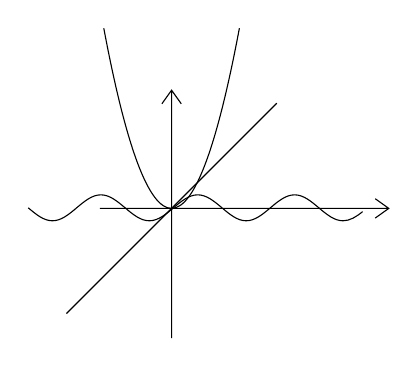
\begin{tikzpicture}[x=0.7pt,y=0.7pt,yscale=-1,xscale=1]
    %uncomment if require: \path (0,300); %set diagram left start at 0, and has height of 300
    
    %Shape: Axis 2D [id:dp21476035781689284] 
    \draw  (165.52,146.23) -- (314.72,146.23)(202.6,85.23) -- (202.6,213.23) (307.72,141.23) -- (314.72,146.23) -- (307.72,151.23) (197.6,92.23) -- (202.6,85.23) -- (207.6,92.23)  ;
    %Shape: Wave [id:dp7563242846602689] 
    \draw   (128.6,145.93) .. controls (132.68,149.37) and (136.58,152.63) .. (141.1,152.63) .. controls (145.62,152.63) and (149.52,149.37) .. (153.6,145.93) .. controls (157.68,142.5) and (161.58,139.23) .. (166.1,139.23) .. controls (170.62,139.23) and (174.52,142.5) .. (178.6,145.93) .. controls (182.68,149.37) and (186.58,152.63) .. (191.1,152.63) .. controls (195.62,152.63) and (199.52,149.37) .. (203.6,145.93) .. controls (207.68,142.5) and (211.58,139.23) .. (216.1,139.23) .. controls (220.62,139.23) and (224.52,142.5) .. (228.6,145.93) .. controls (232.68,149.37) and (236.58,152.63) .. (241.1,152.63) .. controls (245.62,152.63) and (249.52,149.37) .. (253.6,145.93) .. controls (257.68,142.5) and (261.58,139.23) .. (266.1,139.23) .. controls (270.62,139.23) and (274.52,142.5) .. (278.6,145.93) .. controls (282.68,149.37) and (286.58,152.63) .. (291.1,152.63) .. controls (294.73,152.63) and (297.96,150.53) .. (301.2,147.92) ;
    %Shape: Parabola [id:dp3307772220116144] 
    \draw   (167.6,53.23) .. controls (190.93,177.23) and (214.27,177.23) .. (237.6,53.23) ;
    %Straight Lines [id:da017349586183422416] 
    \draw    (148.3,200.53) -- (256.9,91.93) ;
    
\end{tikzpicture}
\end{center}

Examples of functions over the reals $\R$ include $\sin x$ (many-to-one), $x$ (one-to-one), $x^2$ (two-to-one except for the single point $x=0$), etc.

Unfortunately, the term ``function'' is also used to refer to relations that map single points in the domain to possibly multiple points in the range. 
These ``functions'' are called multivalued functions (or multiple-valued functions), and arise prominently in the theory of complex functions, 
where the presence of multiple values engenders the use of so-called branch cuts.

Several notations are commonly used to represent (non-multivalued) functions. 
The most rigorous notation is $f:x\rightarrow f(x)$, which specifies that f is function acting upon a single number $x$ (i.e., f is a univariate, or one-variable, function) and returning a value $f(x)$. 
To be even more precise, a notation like ``$f:R\rightarrow R$, where $f(x)=x^2$''
 is sometimes used to explicitly specify the domain and codomain of the function. 
The slightly different 
``maps to''
 notation $f:x|\rightarrow f(x)$ is sometimes also used when the function is explicitly considered as a 
``map''.


Generally speaking, the symbol $f$ refers to the function itself, while $f(x)$ refers to the value taken by the function when evaluated at a point $x$. 
However, especially in more introductory texts, the notation $f(x)$ is commonly used to refer to the function $f$ itself (as opposed to the value of the function evaluated at $x$). 
In this context, the argument $x$ is considered to be a dummy variable whose presence indicates that the function $f$ takes a single argument (as opposed to $f(x,y)$, etc.). 
While this notation is deprecated by professional mathematicians, it is the more familiar one for most nonprofessionals. 
Therefore, unless indicated otherwise by context, the notation $f(x)$ is taken in this work to be a shorthand for the more rigorous $f:x\rightarrow f(x)$.
}

\begin{mydef}
    \label{mydef:2.1}
    Consider two sets $A$ and $B$, whose elements may be any objects whatsoever, 
    and suppose that with each element $x$ of $A$ there is associated, 
    in some manner, an element of $B$, which we denote by $f(x)$. 
    Then $f$ is said to be a \myKeywordblue{function} from $A$ to $B$ (or a \myKeywordblue{mapping} of $A$ into $B$). 
    The set $A$ is called the \myKeywordblue{domain} of $f$ (we also say $f$ is defined on $A$), 
    and the elements $f(x)$ are called the \myKeywordblue{values} of $f$.
    The set of all values of $f$ is called the \myKeywordblue{range} of $f$.
\end{mydef}
\mybox{\myKeywordblue{Codomain}:  A set within which the values of a function lie (as opposed to the range, which is the set of values that the function actually takes). 

\myKeywordblue{Range}:   If $f:D\rightarrow Y$ is a map (a.k.a. function, transformation, etc.) over a domain $D$, 
then the range of $f$, also called the image of $D$ under $f$, 
is defined as the set of all values that $f$ can take as its argument varies over $D$, i.e.,
\begin{equation*}
    \operatorname{Range}(f)=f(D)={f(\mathbf{X}):\mathbf{X} \in D}.
\end{equation*}

Note that among mathematicians, the word 
``image''
 is used more commonly than 
``range.''


The range is a subset of $Y$ and does not have to be all of $Y$.

Unfortunately, term 
``range''
 is often used to mean domain--its precise opposite--in probability theory, with Feller (1968, p.200) and Evans et al. (2000, p.5) calling the set of values that a variate $X$ can assume (i.e., the set of values $x$ that a probability density function $P(x)$ is defined over) the 
``range''
, denoted by $R_X$ (Evans et al. 2000, p.5).

Even worse, statistics most commonly uses 
``range''
 to refer to the completely different statistical quantity as the difference between the largest and smallest order statistics. In this work, this form of range is referred to as 
``statistical range.''
 
}

\begin{mydef}
    \label{mydef:2.2}
    Let $A$ and $B$ be two sets and let $f$ be a mapping of $A$ into $B$.
    If $E \subset A$, $f(E)$ is defined to be the set of all elements $f(x)$, for $x \in E$. We call $f(E)$ the image of $E$ under $f$. In this notation, $f(A)$ is the range of $f$. It is clear that $f(A) \subset B$. If $f(A) = B$, we say that $f$ maps $A$ \myKeywordblue{onto} $B$. (Note that, according
    to this usage, \myKeywordblue{onto} is more specific than \myKeywordblue{into}.)
    \mybox{onto 满射? into 映射?} 

    If $E \subset B$, $f^{-1}(E)$ denotes the set of all $x \in A$ such that $f(x)\in E$. We call $f^{-1}(E)$ the \myKeywordblue{inverse image} of $E$ under $f$. If $y \in B$, $f^{-1}(y)$ is the set of all $x \in A$ such that $f(x) =y$. If, for each $y\in B$, $f^{-1}(y)$ consists of at most one element of $A$, then $f$ is said to be a 1-1 (\myKeywordblue{one-to-one}) mapping of $A$ into $B$. This may also be expressed as follows: $f$ is a 1-1 mapping of $A$ into $B$ provided that $f(x_1) \neq f(x_2)$ whenever $x_1 \neq x_2$, $x_1 \in A$, $x_2 \in A$.

    (The notation $x_1 \neq x_2$, means that $x_1$ and $x_2$ are distinct elements; otherwise we write $x_1 = x_2$.)
\end{mydef}

\begin{mydef}
    \label{mydef:2.3}
    If there exists a 1-1 mapping of $A$ \myKeywordblue{onto} $B$, we say that $A$ and $B$ can be putin 1-1 correspondence, or that $A$ and $B$ have the same cardinal number, or, briefly, that $A$ and $B$ are equivalent, and we write $A\sim B$. This relation
    clearly has the following properties :

    It is reflexive: $A\sim A$.

    It is symmetric: If $A\sim B$, then $B\sim A$.

    It is transitive: If $A\sim B$ and $B\sim C$, then $A\sim C$.

    Any relation with these three properties is called an equivalence relation.    
\end{mydef}
\mybox{等价关系:
reflexive   自反性,
symmetric   对称性,
transitive  传递性.

集合等势是一种等价关系, 其满足自反性, 对称性, 传递性.}

\begin{mydef}
    \label{mydef:2.4}
    $\forall n\in \mathbb{N}^+$, $J_n = \{1,2,...,n\}$, $J = \{1,2,...,n,...\}$, (set consisting of all positive integers).

    $A$ is finite, $A\sim J_n$ for some n,

    $A = \varnothing$. empty set is also considered to be finite.

    $A$ is infinite, $A$ is not finite.

    $A$ is countable, $A \sim J$
    
    $A$ is uncountable. $A$ is neither finite nor countable.

    countable set and finite set are called at most countable.
\end{mydef}

\mybox{
    \begin{equation*}
        \left\{
        \begin{array}{lll}
        finite & A\sim J_n\\
        infinite &\left\{
            \begin{array}{ll}
                countable& A\sim J\\
                uncountable& \\
            \end{array}
        \right.
        \end{array}
        \right.
    \end{equation*}
    % todo 添加tikz注释
}

countable sets, enumerable, denumerable.

$A, B \in$ finite set\\
$A\sim B$ $\Longleftrightarrow$ $A, B$ contains same number of elements

$A, B \in$ infinite set\\
same number or elements? vague\\
1-1 correspondence. retains its clarity.

\begin{myExample}
    $f:J\rightarrow A$
    \begin{equation*}
        f(n) = \left\{
            \begin{array}{ll}
                \cfrac{n}{2} & (n \text{even})\\
                -\cfrac{n-1}{2} & (n \text{odd})
            \end{array}
        \right.
    \end{equation*}
\end{myExample}
\mybox{$f(n)=(-1)^n\left\lfloor \cfrac{n}{2} \right\rfloor $}

\begin{myRemark}
    a finite set cannot be equivalent to one of its proper subsets, but it's possible for infinite sets.
\end{myRemark}

$J = 1,2,3,4,...$, $A = 0,1,-1,2,-2,...$,$J, A$are infinite sets, $J \subset A$.\\
but there exist a function $f:J\rightarrow A$, $J \sim A$

\begin{mydef}
    \label{mydef:2.7}
    $f(x)$, $x\in J = \mathbb{N}^+$.\\
    $\{x_n\}$, $x_1,x_2,x_3,...$\\
    $x_n$, terms of the sequence.\\
    $\forall n\in J$, $x_n\in A$, $\{x_n\}$ is a sequence in $A$, or a sequence of elements of $A$.
\end{mydef}

every countable set is range of a sequence of distinct terms.
the elements of any countable set can be ``arranged in a sequence''.
replace $J(\mathbb{N}^+)$ by $\mathbb{N} = \{x|, x\in Z,x \geq 0\}$, start with $0$ rather than $1$.

\begin{thm}
    \label{thm:2.8}
    Every infinite subset of a countable set $A$ is countable
\end{thm}

$E\subset A$. $E$ is infinite. 
To prove $E$ is countable, we need a 1-1 correspondation of $J$ to $E$, $f:J\rightarrow E$.
\mybox{
    my first guess is $A$ is a countable set, $A\sim J$ (by def).
    $\exists$ 1-1 mapping $g:$ $J$ onto $A$.
    $x\in J$, $g(x)\in A$.
    $E\subset A$, $\exists  g(x)\in E$.
    $g(x_i)\in E$, $x_i\in J$, $g:J\rightarrow E$.\\
    再证 $x_i$ 不是有限的. $E$ is infinite, there exist infinite $g(x_i)\in E$. $\because g$ is a 1-1 mapping, $\{x_i\}$ is infinite. $\therefore J\sim E$.
}

\begin{proof}
    Suppose $E\subset A$, $E$ is infinite. 
    arrange the elements $x$ of $A$ in a sequence $\{x_n\}$ of a distinct elements. Construct a sequence $n_k$ as follows.\\
    Let $n_1$ be the smallest positive int, s.t. $x_{n_1}\in E$.
    Having chosen $n_1,...n_{k-1}$,$(k=2,3,...)$, let $n_k$ be the smallest integer greater than $n_{k-1}$, s.t. $x_{n_k} \in E$.\\
    Putting $f(k) = x_{n_k}$, $f:J\rightarrow E$ is a 1-1 mapping.
\end{proof}

Countable sets represent the ``smallest'' infinity.

No uncountable set ca be a subset of a countable set.

\mybox{
    rudin 这里尝试区分实无穷与浅无穷, 
    使用集合的势来说明更为具体, 全体整数组成的集合为 ``最小'' 的无穷大, 
    其势为$\aleph_0$, 康托尔使用一一对应关系作为无穷集合之间的等价关系.
    }

\begin{mydef}
    \label{mydef:2.9}
    $\forall \alpha\in A$, $E_\alpha \subset \Omega$, $\{E_\alpha\}$ debites elements of $E_\alpha$. 
    collection of sets (or family of sets)  
    \mybox{sets of sets sounds strange}  
    union
    \begin{equation}
        \label{eq:2.1}
        S = \bigcup_{\alpha\in A} E_\alpha
    \end{equation}
    if $A$ consists of the integers $1,2,...,n$.
    \begin{equation}
        \label{eq:2.2}
        S = \bigcup_{m=1}^n E_m
    \end{equation}
    \begin{equation}
        \label{eq:2.3}
        S = E_1 \bigcup E_2 \bigcup \cdots \bigcup E_n.
    \end{equation}
    if $A$ is the set of all positive integers.
    \begin{equation}
        \label{eq:2.4}
        S = \bigcup_{m=1}^{\infty} E_m.
    \end{equation}
    intersection
    \begin{equation}
        \label{eq:2.5}
        P = \bigcap_{\alpha\in A} E_\alpha
    \end{equation}
    \begin{equation}
        \label{eq:2.6}
        S = \bigcap_{m=1}^n E_m = E_1 \cap E_2 \cap \cdots \cap E_n.
    \end{equation}
    \begin{equation}
        \label{eq:2.7}
        S = \bigcap_{m=1}^{\infty} E_m.
    \end{equation}

    $A$ and $B$ intersect if $A\bigcap B$ is not empty, otherwise they are disjoint.
\end{mydef}

\begin{myExample}
    some example of set relation
\end{myExample}

\begin{myRemark}
    Many properties of unions and intersections are quite similar to those of sums and products; in fact, the words sum and product were sometimes used in this connection, and the symbols $\sum$ and $\prod$ were written in place of $\bigcup$ and $\bigcap$.
\end{myRemark}

The commutative and associative laws are trivial:
\begin{align}
        A \cup B &= B \cup A; &
        A \cap B &= B \cap A \label{eq:2.8} \\
        \left(A \cup B\right) \cup C &= A \cup \left(B \cup C\right); &
        \left(A \cap B\right) \cap C &= A \cap \left(B \cap C\right);\label{eq:2.9}
\end{align}

Thus the omission of parentheses in \ref{eq:2.3} and \ref{eq:2.6} is justified.

The distributive law also holds:
\begin{equation}
    \label{eq:2.10}
    A \cap \left( B \cup C\right) = 
    \left(A \cap B\right) \cup \left(A \cap C\right).
\end{equation}
To prove this, let the left and right members of \ref{eq:2.10} be denoted by $E$ and $F$, respectively.

Suppose $x \in E$. Then $x \in A$ and $x \in B \cup C$, that is, $x \in B$ or$ x \in C$ (possibly both). Hence $x \in A\cap B$ or $x \in A\cap C$, so that $x \in F$. Thus $E \subset F$.

Next, suppose $x \in F$. Then $x \in A\cap B$ or $x \in A\cap C$. That is, $x \in A$, and $x \in B\cup C$. Hence $x \in A\cap \left(B \cup C\right)$, so that $F \subset E$.

It follows that $E = F$.

We list a few more relations which are easily verified:

\begin{align}
    A \subset A \cup B, \label{eq:2.11}\\
    A \cap B \subset B, \label{eq:2.12}
\end{align}

If $0$ denotes the empty set, then
\begin{equation}
    \begin{array}{cc}
        A \cup 0 = A, & A \cap 0 = 0.
    \end{array}
\end{equation}
If $A \subset B$, then
\begin{equation}
    \begin{array}{cc}
        A \bigcup B = B, & A \bigcap B = A.
    \end{array}
\end{equation}

\mybox{现在一般使用 $\varnothing$ 指代空集}


\begin{thm}
    \label{thm:2.12}
    Let $\{E_n\}, n=1,2,3,...,$ be a sequence of countable sets, and put
    \begin{equation}
        \label{eq:2.15}
        S = \bigcup_{n=1}^{\infty} E_n.
    \end{equation}
    Then S is countable.
\end{thm}
\mybox{
    将 $E_n$ 按顺序排成一张表格, 按反对角线重新排列成新的序列, 
    得到 $T$, $S\sim T$.
    $S$ is at most countable.
    同时存在无限集合(infinite set) $E_1$, $E_1 \subset S$, 
    $S$ is countable.
}

\begin{proof}
    Let every set $E_n$ be arranged in a sequence $\sequence{x_{nk}}$, 
    $k = 1,2,3,\dots$,
    and consider the infinite array
    \begin{equation}
        \label{eq:2.16}
        \begin{array}{ccccc}
            x_{11} & x_{12} & x_{13} & x_{14} & \cdots \\  
            x_{21} & x_{22} & x_{23} & x_{24} & \cdots \\  
            x_{31} & x_{32} & x_{33} & x_{34} & \cdots \\  
            x_{41} & x_{42} & x_{43} & x_{44} & \cdots \\  
            \cdots & \cdots & \cdots & \cdots & \cdots \\
        \end{array}
    \end{equation}
    in which the elements of $E_n$ form the $n$th row. 
    The array contains all elements of $S$.
    As indicated by the arrows, 
    these elements can be arranged in a sequence
    \begin{equation}
        \label{eq:2.17}
        x_{11};
        x_{21}, x_{12};
        x_{31}, x_{22}, x_{13};
        x_{41}, x_{32}, x_{23}, x_{14};
        \cdots
    \end{equation}
    
    If any two of the sets En have elements in common, 
    these will appear more than once in (\ref{eq:2.17}). 
    Hence there is a subset $T$ of the set of all positive integers 
    such that $S \sim T$, 
    which shows that $S$ is at most countable (Theorem \ref{thm:2.8}). 
    Since $E_1 \subset S$, and $E_1$ is infinite, 
    $S$ is infinite, and thus countable.
\end{proof}

\begin{myCorollary*}
    Suppose $A$ is at most countable, and, for every $\alpha \in A, B$, is at most countable. Put
    \begin{equation*}
        T = \bigcup_{\alpha\in A} B_\alpha.
    \end{equation*}
    Then T is at most countable.
\end{myCorollary*}

For $T$ is equivalent to a subset of \ref{eq:2.15}.

\begin{thm}
    \label{thm:2.13}
    Theorem Let $A$ be a countable set, and let $B_n$ be the set of all $n$-tuples $(a_1, ...,a_n)$, where $a_k \in  A (k=1,...,n)$, and the elements $a_1, ...,a_n$ need not be distinct. Then $B_n$ is countable.
\end{thm}

\begin{proof}
    That $B_1$ is countable is evident, since $B_1 = A$. 
    Suppose $B_{n-1}$ is countable $(n = 2, 3, 4, ... )$. 
    The elements of $B_n$ are of the from
    \begin{equation}
        \label{eq:2.18}
        (b,a)
        \quad
        (b \in B_{n-1},a \in A).
    \end{equation}
    For every fixed $b$, the set of pairs $(b, a)$ is equivalent to $A$, and hence countable. 
    Thus $B_n$ is the union of a countable set of countable sets. 
    By Theorem \ref{thm:2.12}, Bn is countable.
The theorem follows by induction.
\end{proof}

\begin{myCorollary*}
    The set of all rational numbers is countable.
\end{myCorollary*}

\begin{proof}
    We apply Theorem \ref{thm:2.13}, 
    with $n = 2$, noting that every rational $r$ is of the form $b / a$, 
    where $a$ and $b$ are integers. 
    The set of pairs $(a, b)$, 
    and therefore the set of fractions $b / a$, is countable.
\end{proof}

In fact, even the set of all algebraic numbers is countable (see Exercise 2).

That not all infinite sets are, however, countable, is shown by the next
theorem.

\begin{thm}
    \label{thm:2.14}
    Theorem Let $A$ be the set of all sequences whose elements are the digits $0$ and $1$. This set $A$ is uncountable. 
\end{thm}

The elements of $A$ are sequences like $1, 0, 0, 1, 0, 1, 1, 1, ... .$

\begin{proof}
    Let $E$ be a countable subset of $A$, 
    and let $E$ consist of the sequences $s_1, s_2 , s_3 , ...$. 
    We construct a sequences as follows. 
    If the $n$th digit in $s_n$ is $1$, 
    we let the $n$th digit of $s$ be $0$, and vice versa. 
    Then the sequence $s$ differs from every member of $E$ in at least one place; hence $s \not\in E$. 
    But clearly $s \in A$, so that $E$ is a proper subset of $A$.

    We have shown that 
    every countable subset of $A$ is a proper subset of $A$. 
    It follows that $A$ is uncountable 
    (for otherwise $A$ would be a proper subset of $A$, which is absurd).
\end{proof}

The idea of the above proof was first used by Cantor, 
and is called Cantor's diagonal process; 
for, if the sequences $s_1, s_2 , s_3 ,\dots$ are placed in an array like (\ref{eq:2.16}), 
it is the elements on the diagonal which are involved in the construction of the new sequence.

Readers who are familiar with the binary representation of the real numbers (base 2 instead of 10) will notice that 
Theorem \ref{thm:2.14} implies that the set of all real numbers is uncountable. 
We shall give a second proof of this fact in Theorem \ref{thm:2.43}.
    % chap03.tex
\chapter{Numerical sequences and series}
% chap03sec01.tex
\section{Convergent sequences}

\begin{myDef}\label{myDef:3.1 converge}
    A sequences 
    $\{p_n\}$ 
    in metric space $X$ is said to converge if there is a point $p \in X$ with the following property:
    
    For every $\varepsilon >0$ there is an integer $N$ s.t. $n \geq N$ implies that $d(p_n, p) < \varepsilon$. (Here $d$ denotes the distance in $X$.)

    In this case we also say that $\{p_n\}$ converges to $p$, or that $p$ is the limit of $\{p_n\}$. [see Th 3.2(b)], and we write $p_n \rightarrow p$, or

    \begin{equation*}
        \lim_{n \to \infty} p_n = p.
    \end{equation*}

    if $\{p_n\}$ does not converge, it is said to diverge.
\end{myDef}

our definition of ``convergent sequence'' depends not only on $\{p_n\}$ but also on $X$. For instance, the sequence $\{1/n\}$ converges in $\mathbb{R}^1$(to $0$), but fails to converge in the set of all positive real numbers [with $d(x,y) = |x-y|$]. 
In cases of possible ambiguity, we can be more
precise and specify ``convergent in $X$'' rather than ``convergent''.

we recall that the set of all points $p_n (n=1,2, 3,...)$ is the range of 
$\{p_n\}$.
The range of a sequence may be a finite set, or it may be infinite. The sequence
$\{p_n\}$ is said to be bounded if its range is bounded.

As examples, consider the following sequences of complex numbers
(that is, $X = \mathbb{R}^2$):

\begin{enumerate}[(a)]
    \item If $s_n=1/n$, then $\lim_{n \to \infty} s_n = 0$; the range is infinite, and the sequence is bounded.
    \item If $s_n=n^2$ the sequence $\{s_n\}$ is unbounded, is divergent, and has infinite range.
    \item If $s_n = 1+[(- 1)^n/n]$, the sequence $\{s_n\}$ converges to $1$, is bounded, and has infinite range.
    \item If $s_n =i^n$ the sequence $\{s_n\}$ is divergent, is bounded, and has finite range.
    \item If $s_n = 1(n=1,2,3,...)$, then $\{s_n\}$ converges to $1$, is bounded, and has finite range.
\end{enumerate}

% We now summarize some important properties of convergent sequences in metric spaces.

\begin{thm}\label{thm:3.2 convergence sequence in metric space}
    Let$\{p_n\}$ be a sequence in a metric space $X$.
    \begin{enumerate}[(a)]
        \item $\{p_n\}$ converges to $p \in X$ if and only if every neighborhood of $p$ contains $p_n$ for all but finitely many $n$.
        \item If $p\in X$, $p^\prime \in X$, and if $\{p_n\}$ converges to $p$ and to $p'$, then $p^\prime =p$.
        \item If $\{p_n\}$ converges, then $\{p_n\}$ is bounded.
        \item If $E \subset X$ and if $p$ is a limit point of $E$, then there is a sequence$\{p_n\}$ in $E$ such that $p = \lim_{n \to \infty} p_n$.
    \end{enumerate}
\end{thm}

\begin{proof}
    (d) For each positive integer $n$, there is a point $p_n \in E$ such that $d(p_n,p) <1/n$. Given $\varepsilon > 0$, choose $N$ so that $N \varepsilon >1$. If $n>N$, it follows that $d(p_n, p) <\varepsilon$. Hence $p_n \rightarrow p$.
\end{proof}

\begin{thm}\label{thm:3.3}
    Suppose $\{s_n\}, \{t_n\}$ are complex sequences, and 
    $\lim_{n \to \infty} s_n = s$,
    $\lim_{n \to \infty} t_n = t$.
    Then
    \begin{enumerate}[(a)]
        \item $\lim_{n \to \infty} (s_n + t_n) = s + t$;
        \item $\lim_{n \to \infty} c s_n = cs$, $\lim_{n \to \infty} (c + s_n) = c + s$, for any number $c$;
        \item $\lim_{n \to \infty} s_n t_n = st$;
        \item $\lim_{n \to \infty} \frac{1}{s_n} = \frac{1}{s}$, provided $s_n \neq 0(n = 1,2,3,\dots)$, and $s \neq 0$.
    \end{enumerate}
\end{thm}

\myproof{
    \begin{equation}
        \label{eq:3.1}
        s_n t_n - st = (s_n - s)(t_n - t) + s(t_n - t) + t(s_n - s).
    \end{equation}
}

\begin{thm} As:\\
    \label{thm:3.4}
    (a) Suppose $\mathbf{x}_n \in R^k (n = 1,2,3,\dots)$ and
    \begin{equation*}
        \mathbf{x_n} = (
            \alpha_{1,n},\dots
            \alpha_{k,n}
        ).
    \end{equation*}
    Then $\{\mathbf{x}_n\}$ converges to $\mathbf{x} = (\alpha_1, \dots, \alpha_k)$ if and only if
    \begin{equation}
        \lim_{n \to \infty} \alpha_{j,n} = \alpha_j \qquad (1\leq j\leq k).
    \end{equation}

    (b) Suppose $\{\mathbf{x}_n\}$, $\{\mathbf{y}_n\}$ are sequences in $\mathbb{R}^k$, $\{\beta_n\}$ is a sequence of real numbers, and 
    $\mathbf{x}_n \rightarrow \mathbf{x}$,
    $\mathbf{y}_n \rightarrow \mathbf{y}$,
    $\beta_n \rightarrow \beta$. Then
    \begin{equation*}
        \lim_{n \to \infty} (\mathbf{x_n} + \mathbf{y_n}) = \mathbf{x} + \mathbf{y}, \quad
        \lim_{n \to \infty} \mathbf{x_n} \cdot \mathbf{y_n} = \mathbf{x} \cdot \mathbf{y}, \quad
        \lim_{n \to \infty} \beta_n \mathbf{x_n} = \beta \mathbf{x}.
    \end{equation*}
\end{thm}

% chap03sec02

\section{Subsequences}
\begin{mydef}\label{def:3.5}
    Given a sequence $\{p_n\}$, consider a sequence $\{n_k\}$ of positive integers, such that $n_1 <n_2 <n_3 <....$ Then the sequence $\{p_{n_i}\}$ is called a \emph{subsequence} of $\{p_n\}$. If $\{p_{n_i}\}$ converges, its limit is called a subsequential limit of $\{p_n\}$.
\end{mydef}
It is clear that $\{p_n\}$ converges to $p$ if and only if every subsequence of $\{p_{n}\}$ converges to $p$. We leave the details of the proof to the reader.

\begin{thm}\label{thm:3.6}
    (a) If $\{p_{n}\}$ is a sequence in a compact metric space $X$, then some subsequence of $\{p_{n}\}$ converges to a point of $X$.

    (b) Every bounded sequence in $\R^k$ contains a convergent subsequence.
\end{thm}

\begin{thm}\label{thm:3.7}
    The subsequential limits of a sequence $\{p_{n}\}$  in a metric space $X$ form a closed subset of $X$.
\end{thm}


% chap03sec03
\section{Cauchy sequences}
\begin{myDef}\label{myDef:3.8}
    A sequence $\{p_n\}$ in a metric space $X$ is said to be a \emph{Cauchy sequence} if for every $\varepsilon > 0$ there is an integer $N$ such that $d(p_n, p_m) <e$ if $n \geq N$ and $m \geq N$. 
\end{myDef}

% $\R{1}$
In our discussion of Cauchy sequences, as well as in other situations
which will arise later, the following geometric concept will be useful.

\begin{myDef}\label{myDef:3.9}
    % 3.9 Definition 
    Let $E$ be a nonempty subset of a metric space $X$, and let $S$ be the set of all real numbers of the form $d(p, q)$, with $p \in E$ and $q \in E$. The sup of $S$ is called the diameter of $E$.    
\end{myDef}

If $\sequence{p_n}$ is a sequence in $X$ and if $E_N$ consists of the points $p_N, p_{N+1}, p_{N+2},\dots$, it is clear from the two preceding definitions that $\sequence{p_n}$ is a \emph{Cauchy sequence} \emph{if and only if}

\begin{equation*}
    \lim_{N \to \infty} \text{diam } E_N = 0.
\end{equation*}

\begin{thm}\label{thm:3.10}
    (a) If $\bar{E}$ is the closure of a set $E$ in a metric space $X$, then 
    \begin{equation*}
        \rm{diam }\; E = \rm{diam }\; E.
    \end{equation*}
    
    (b) If $K_n$ is a sequence of compact sets in $X$ such that $K_n \supset K_{n+1} $ $(n=1,2,3,...) $and if
    \begin{equation*}
        \lim_{n \to \infty} \rm {diam }\; K_n = 0,
    \end{equation*}
    then $\cap_1^\infty K_n$ consists of exactly one point.
\end{thm}

% https://blog.sciencenet.cn/blog-783377-668028.html
% latex斜体变正体需在代码前加 rm
% y=exp(log(x+1))
% 代码:y=exp(log(x+1))
% y=exp(log(x+1))
% 代码:\rm y=exp(log(x+1))
% y=exp(log(x+1))
% 代码:y={rm exp}({rm log}(x+1))
% {}可以控制作用域的范围

\begin{thm}\label{thm:3.11}
    (a) Inany metric space $X$, every convergent sequence is a Cauchy sequence.

    (b) If $X$ is a compact metric space and if $\sequence{p_n}$ is a Cauchy sequence in $X$, then $\sequence{p_n}$ converges to some point of $X$.

    (c) In $\R{k}$, every Cauchy sequence converges.
\end{thm}

Note: The difference between the definition of convergence and
the definition of a Cauchy sequence is that the limit is explicitly involved
in the former, but not in the latter. Thus Theorem 3.11(b) may enable us
to decide whether or not a given sequence converges without knowledge
of the limit to which it may converge.

The fact (contained in Theorem 3.11) that a sequence converges in
$\R{k}$ if and only if it is a Cauchy sequence is usually called the 
\emph{Cauchy criterion} for convergence.

\begin{myDef}\label{myDef:3.12}
    A metric space in which every Cauchy sequence converges is
    said to be \emph{complete}.
\end{myDef}


Thus Theorem 3.11 says that \emph{all compact metric spaces and all Euclidean spaces are complete}. Theorem 3.11 implies also that every closed subset $E$ of a complete metric space $X$ is complete. (Every Cauchy sequence in $E$ is a Cauchy sequence in $X$. hence it converges to some $p \in X$, and actually $p \in E$ since $E$ is closed.) An example of a metric space which is not complete is the space of all
rational numbers, with $d(x, y) = |x - y|$.

Theorem 3.2(c) and example (d) of Definition 3.1 show that convergent sequences are bounded, but that bounded sequences in $\R{k}$ need not converge. However, there is one important case in which convergence is equivalent to boundedness; this happens for monotonic sequences in $\R{1}$.


\begin{myDef}\label{myDef:3.13}
    A sequence $\sequence{s_n}$ of real numbers is said to be

    (a) monotonically increasing if $s_n \leq s_{n+1}$ $(n=1,2,3,...)$;

    (b) monotonically decreasing if $s_n \geq s_{n+1}$ $(n=1,2,3,...)$.
\end{myDef}

\begin{thm}\label{thm:3.14}
    Theorem Suppose $\sequence{s_n}$ is monotonic. Then $\sequence{s_n}$ converges if and only if it is bounded.
\end{thm}

% chap03sec04
\section{Upper and lower limits}

\begin{myDef}
    \label{myDef:3.15}
    Let $\sequence{s_n}$ be a sequence of real numbers with the following property: For every real $M$ there is an integer $N$ such that $n > N$ implies $s_n \geq M$. We then write
    \begin{equation*}
        s_n \rightarrow +\infty.
    \end{equation*}
    Similarly, if for every real $M$ there is an integer $N$ such that $n > N$ implies $s_n \leq M$, we write
    \begin{equation*}
        s_n \rightarrow -\infty.
    \end{equation*}
\end{myDef}

It should be noted that we now use the symbol $rightarrow$ (introduced in Definition 3.1) for certain types of divergent sequences, as well as for convergent sequences, but that the definitions of convergence and of limit, given in Definition 3.1, are in no way changed.

\begin{myDef}
    \label{myDef:3.16}
    Let $\sequence{s_n}$ be a sequence of real numbers. Let $E$ be the set of numbers $x$ (in the extended real number system) such that $s_n rightarrow x$ for some subsequence $\sequence{s_n}$. This set $E$ contains all subsequential limits as defined in Definition 3.5, plus possibly the numbers $+\infty, -\infty$.

    We now recall Definitions 1.8 and 1.23 and put
    \begin{align*}
        s^{*} = \sup E,
        s_{*} = \inf E,
    \end{align*}
    The numbers $s^{*}, s_{*}$, are called the upper and lower limits of $\sequence{s_n}$; we use the notation 
    \begin{equation*}
        \limsup_{n \rightarrow \infty} s_n = s^{*},\quad \liminf_{n \rightarrow \infty} s_n = s_{*}.        
    \end{equation*}
\end{myDef}
% chap03sec05
\section{Some special sequences}

some sequences occur frequently.
remark: If $0\leq x_n \leq s_n$ for $n \geq N$, where $N$ is some fixed number, and if $s_n \rightarrow 0$, then $x_n \rightarrow 0$.

\begin{thm}
    \label{thm:3.20}
    (a) If $p > 0$, then $\lim_{n \to \infty} \frac{1}{n^p} = 0$. 

    (b) If $p > 0$, then $\lim_{n \to \infty} \sqrt[n]{p} = 1$.
    
    (c) $\lim_{n \to \infty} \sqrt[n]{n} = 1$.
    
    (d) If $p > 0$ and $\alpha$ is real, then $\lim_{n \to \infty} \frac{n^\alpha}{(1+p)^n} = 0$.

    (e) If $|x|<1$, then $\lim_{n \to \infty} x^n = 0$.
\end{thm}
% chap03sec06
\section{Series}
Consider complex-valued sequences and series

\begin{mydef}
    \label{def:3.21}
    Given a sequence $\sequence{a_n}$, we use the notation
    \begin{equation*}
        \sum_{n=p}^{q} a_n \quad (p \leq q)
    \end{equation*}
    to denote the sum $a_p+a_{p+1}+\dots+a_q$. With $\sequence{a_n}$ we associate a sequence $\sequence{s_n}$, where
    \begin{equation*}
        s_n = \sum_{k=1}^{n} a_k.
    \end{equation*}
    For $\sequence{s_n}$ we also use the symbolic expression
    \begin{equation*}
        a_1 + a_2 + a_3 + \dots
    \end{equation*}
    or, more concisely
    \begin{equation}
        \sum_{n=1}^{\infty} a_n.
    \end{equation}
    we call this \emph{infinite series}, or just a \emph{series}. The numbers $\sequence{s_n}$ are called the \emph{partial sums} of the series. If $\sequence{s_n}$ converges to $s$, we say that that the series \emph{converges}, and write
    \begin{equation*}
        \sum_{n=1}^{\infty} a_n = s.
    \end{equation*}
    The number $s$ is called the sum of the series; but it should be clearly understood that $s$ is the \emph{limit of a sequence of sums}, and is not obtained simply by addition.
    
    If $\sequence{s_n}$ diverges, the series is said to diverge.

    Sometimes, for convenience of notation, we shall consider series of the form
    \begin{equation}
        \sum_{n=0}^{\infty} a_n.
    \end{equation}
    And frequently, when there is no possible ambiguity, or when the distinction is immaterial, we shall simply write $\sum a_n$ , in place of (4) or (5).

    It is clear that every theorem about sequences can be stated in terms of series (putting $a_1 = s_1$, and $a_{n} = s_{n} - s_{n-1}$ for $n > 1$), and vice versa. But it is nevertheless useful to consider both concepts.
\end{mydef}
The Cauchy criterion (Theorem 3.11) can be restated in the following form:
    
\begin{thm}
    \label{thm:3.22}
    $\sum a_n$  converges if and only if for every $\varepsilon \in > 0$ there is an integer $N$ such that
    \begin{equation}
        \left|
            \sum_{k=n}^{m} a_k 
        \right| \leq \varepsilon
    \end{equation}
    if $m \geq n \geq N$. 
\end{thm}

In particular, by taking $m = n$, (6) becomes
\begin{equation*}
    |a_n| \leq \varepsilon \quad (n \geq N).
\end{equation*}

\begin{thm}
    \label{thm:3.23}
    If $\sum a_n$ converges, then $\lim_{n \rightarrow \infty} a_n = 0$. 
\end{thm}

The condition $a_n \rightarrow 0$ is not sufficient to ensure convergence of $\sum a_n$. For instance, the series
\begin{equation*}
    \sum_{n=1}^{\infty}\frac{1}{n}
\end{equation*}
diverges; for the proof we refer to Theorem 3.28.

Theorem 3.14, concerning monotonic sequences, also has an immediate
counterpart for series.
\begin{thm}
    \label{thm:3.24}
    A series of nonnegative terms converges if and only if its partial sums form a bounded sequence.
\end{thm}

\begin{thm}
    \label{thm:3.25}
    (a) If $|a_n| \leq c_n$, for $n \geq N_0$, where $N_0$ is some fixed integer, and if $\sum c_n$ converges, then $\sum a_n$ converges.

    (b) If $a_n \geq d_n \geq 0$ for $n \geq N_0$, and if $\sum d_n$, diverges, then $\sum a_n$ diverges.
\end{thm}

\mybox{比较审敛法}
% chap03sec07
\section{Series of nonnegative terms}

\begin{thm}
    \label{thm:3.26}
    If $0 \leq x < 1$, then
    \begin{equation*}
        \sum_{n=0}^{\infty} x^n = \frac{1}{1-x}.
    \end{equation*}
    If $x \geq 1$, the series diverges. 
\end{thm}

\mybox{几何级数收敛条件}


\mybox{Cauchy use ``thin'' subsequence of $\sequence{a_n}$ determines the convergence or divergence of $\sum a_n$}

\begin{thm}
    \label{thm:3.27 Cauchy}
    Suppose $a_1 \geq a_2 \geq a_3 \geq \dots \geq 0$.
    Then the series $\sum_{n=1}^{\infty}a_n$ converges if and only if the series
    \begin{equation}
        \sum_{k=0}^{\infty} 2^k a_{2^k}
        = a_1 + 2 a_2 + 4 a_4 + 8 a_8 + \dots
    \end{equation}
    converges.
\end{thm}

\begin{proof}
    By Theorem \ref{thm:3.24}, it suffices to consider boundedness of the partial sums.
    Let
    \begin{align*}
        s_n &= a_1 + a_2 + \dots + a_n, \\
        t_n &= a_1 + 2 a_2 + \dots + 2^{k} a_{2^k}.
    \end{align*}
    For $n < 2^k$,
    \begin{align*}
        s_n 
        &\leq a_1 + (a_2 + a_3) + \dots + (a_{2^k}+\dots+a_{2^{k+1}-1}) \\
        &\leq a_1 + 2a_2 + \dots + 2^k a_{2^k} \\
        &= t_k,
    \end{align*}
    so that
    \begin{equation}
        \label{3.8}
        s_n \leq t_k.
    \end{equation}
    On the other hand, if $n > 2^k$,
    \begin{align*}
        s_n 
        &\geq a_1 + a_2 + (a_3 + a_4) + \dots + (a_{2^{k-1}+1}+\dots+a_{2^{k}}) \\
        &\geq \frac{1}{2}a_1 + a_2 + 2 a_4 + \dots + 2^{k+1} a_{2^k} \\
        &= \frac{1}{2}t_k,
    \end{align*}
    so that
    \begin{equation}
        \label{eq:3.9}
        2 s_n \geq t_k.
    \end{equation}
    $\sequence{s_n}$,
    $\sequence{t_n}$ are both bounded or both unbounded.
\end{proof}

\begin{thm}
    \label{thm:3.28}
    $\sum \frac{1}{n^p}$ converges if $p>1$ and diverges if $p\leq 1$. 
\end{thm}

\begin{thm}
    \label{thm:3.29}
    If $p > 1$ ,
    \begin{equation}
        \label{eq:3.10}
        \sum_{n=2}^{\infty} \frac{1}{n (\log n)^p}
    \end{equation}
    converges; if $p \leq 1$ , the series diverges.
\end{thm}

``$\log n$'' the logarithm of $n$ to the base $e$ (compare Exercise 7, Chap. 1);
the number $e$ will be defined in a moment (see Def 3.30). We let the series start with $n=2$ , since $\log 1 = 0$ .

\begin{proof}
    The monotonicity of the logarithmic function (which will be discussed in more detail in Chap. 8) implies that ($\log n$) increase. Hence ($1/n \log n$) decreases, and we can apply Theorem \ref{thm:3.27 Cauchy} to (\ref{eq:3.10}); this leads us the series
    \begin{equation}
        \label{eq:3.11}
        \sum_{k=1}^{\infty}2^k\cdot\frac{1}{2^k (\log 2^k)^p} = 
        \sum_{k=1}^{\infty}\cdot\frac{1}{(k\log 2)^p} =
        \frac{1}{(\log 2)^p}\sum_{k=1}^{\infty}\cdot\frac{1}{k^p}
    \end{equation}
    and Theorem \ref{thm:3.29} follows from Theorem \ref{thm:3.28}.
\end{proof}


This procedure may evidently be continued. For instance,
\begin{equation}
    \label{eq:3.12}
    \sum_{n=3}^{\infty}\frac{1}{n \log n \log \log n}
\end{equation}
diverges, whereas
\begin{equation}
    \label{eq:3.13}
    \sum_{n=3}^{\infty}\frac{1}{n \log n (\log \log n)^2}
\end{equation}
converges.

Series (\ref{eq:3.12}) differ very littel from (\ref{eq:3.13}). Still, one diverges, the other converges.
If we continue the process which led us from Theorem \ref{thm:3.28} to Theorem \ref{thm:3.29}, we get pairs of convergent and divergent series whose terms differ even less than those of (\ref{eq:3.12}) and (\ref{eq:3.13}).
One might thus be led to the conjecture that there is a limiting situation of some sort, a ``boundary'' with all convergent series on one side, all divergent series on the other side --- at least as far as series with monotonic coefficients are converned. 
This notion of ``boundary'' is of course quite vague.
The point we wish to make is this: No matter how we make this notion precise, the conjecture is false. Exercises 11(b) and 12(b) may serve as illustrations.

More deeper aspect of convergence theory can refer to Knopp's \emph{``Theory and Application of Infinite Series''}, Chap IX, particularly Sec. 41.

% chap03sec08
\section{The number $e$}

\begin{myDef}
    \label{myDef:3.30 e}
    $e = \sum_{n=0}^{\infty}\frac{1}{n!}.$

    Here $n! = 1 \cdot 2 \cdot 3 \cdots n$ if $n \geq 1$ , and $0! = 1$.  
\end{myDef}

Since
\begin{align*}
    s_n
    &= 1 + 1 
    + \frac{1}{1 \cdot 2} 
    + \frac{1}{1 \cdot 2 \cdot 3} 
    + \cdots 
    + \frac{1}{1 \cdot 2 \cdots n} \\
    &< 1 + 1
    + \frac{1}{2}
    + \frac{1}{2^2}
    + \cdots
    + \frac{1}{2^{n-1}} 
    < 3
\end{align*}
The series converges, and the definition makes sense. In fact, the series converges very rapidly and allows us to compute $e$ with great accuracy.

It is of interest to note that $e$ can also be difined by means of another limit process; the proof provides a good illustration of operations with limits:

\begin{thm}
    \label{thm:3.31 another def of e}
    $\lim_{n \to \infty} (1+1/n)^n = e.$ 
\end{thm}
\mybox{Is this equation found by Bernoulli?}
\begin{proof}
    Let
    \begin{equation*}
        s_n = \sum_{k=0}^{n} \frac{1}{k!}, \quad
        t_n = \sum_{k=0}^{n} (1 + \frac{1}{n})^n. 
    \end{equation*}
    by the binomial theorem,
    \begin{align*}
        t_n &= 1 + 1
        + \frac{1}{2!}\left(1 - \frac{1}{n}\right)
        + \frac{1}{3!}\left(1 - \frac{1}{n}\right)\left(1 - \frac{2}{n}\right)
        + \cdots \\
        &+ \frac{1}{n!}\left(1 - \frac{1}{n}\right)\left(1 - \frac{2}{n}\right)\cdots\left(1-\frac{n-1}{n}\right).
    \end{align*}
    Hence $t_n \leq s_n$ , so that
    \begin{equation}
        \label{eq:3.14}
        \limsup_{n \rightarrow \infty}  t_n \leq e,
    \end{equation}

    by Theorem \ref{thm:3.19}. Next, if $n \geq m$ ,
    \begin{equation*}
        t_n \geq 1 + 1
        + \frac{1}{2!}\left(1 - \frac{1}{n}\right)
        + \cdots
        + \frac{1}{m!}\left(1-\frac{1}{n}\right)
        + \cdots
        + \frac{1}{m!}\left(1-\frac{1}{n}\right)\cdots\left(1-\frac{m-1}{n}\right).
    \end{equation*}

    Let $n \rightarrow \infty$ , kepping $m$ fixed. We get 
    \begin{equation*}
        \liminf_{n \to \infty} t_n \geq 1 + 1 
        + \frac{1}{2!}
        + \cdots
        + \frac{1}{m!},
    \end{equation*}
    so that
    \begin{equation*}
        s_m \leq \liminf_{n \rightarrow \infty} t_n,
    \end{equation*}
    Letting $m \rightarrow \infty$, we finally get
    \begin{equation}
        \label{eq:3.15}
        e \leq \liminf_{n \rightarrow \infty} t_n.
    \end{equation} 
    
    The Theorem follows from (\ref{eq:3.14}) and (\ref{eq:3.15}).
\end{proof}

The rapidly with which the series $\sum 1/n!$ converges can be estimated as follows: If $s_n$ has the same meaning as above, we have
\begin{align*}
    e - s_n
    &= \frac{1}{(n+1)!}
    + \frac{1}{(n+2)!}
    + \frac{1}{(n+3)!}
    + \cdots \\
    &< \frac{1}{(n+1)!}\left\{
        1
        + \frac{1}{n+1}
        + \frac{1}{(n+1)^2}
        + \cdots
    \right\} = \frac{1}{n!n}
\end{align*}
so that
\begin{equation}
    \label{eq:3.16}
    0 < e - s_n < \frac{1}{n!n}.
\end{equation}
Thus $s_{10}$, for instance, approximates $e$ with an error less than $10^{-7}$.
The inequality (\ref{eq:3.16}) is of theoretical interest as well, since it enables us to prove the irrationality of $e$ very easily.

\begin{thm}
    \label{thm:3.32}
    $e$ is irrational.
\end{thm}

\begin{proof}
    Suppose $e$ is rational. Then $e = p/q$, where $p$ and $q$ are positive integers. 
    By (\ref{eq:3.16}),
    \begin{equation}
        \label{eq:3.17}
        0<q!(e-s_q)<\frac{1}{q}.
    \end{equation}
    By our assumption, $q!e$ is an integer. Since
    \begin{equation*}
        q!s_q = 
        q!\left(
            1 + 1 + \frac{1}{2!} + \cdots + \frac{1}{q!}
        \right)
    \end{equation*}
    is an integer, we see that $q!(e-s_q)$ is an integer.

    Since $q \geq 1$, (\ref{eq:3.17}) implies the existence of an integer between $0$ and $1$. We have thus reached a contradiction.
\end{proof}

Actually, $e$ is not even an algebraic number.
For a simple proof of this, see page 25 of Niven's book, or page 176 of Herstein's, cited in the Bibliography.

% \input{chap/chap03mynotes.tex}
    % chap04

\chapter{Continuity}

The function concept and some of the related terminology were introduced in
Definitions \ref{myDef:2.1} and \ref{myDef:2.2}. Although we shall (in later chapters) be mainly interested in real and complex functions (i.e., in functions whose values are real or complex numbers) we shall also discuss vector-valued functions (i.e., functions with values in $\R{k}$) and functions with values in an arbitrary metric space. The theorems we shall discuss in this general setting would not become any easier if we restricted ourselves to real functions, for instance, and it actually simplifies and clarifies the picture to discard unnecessary hypotheses and to state and prove theorems in an appropriately general context. 

The domains of definition of our functions will also be metric spaces, suitably specialized in various instances.

% chap04sec01
\section{Limits of functions}

\begin{myDef}
    \label{myDef:4.1}
    Let $X$ and $Y$ be metric spaces; suppose $E \subset X$, $f$ maps $E$ into $Y$, and $p$ is a limit point of $E$. We write $f(x) \rightarrow q$ as $x \rightarrow p$, or
    \begin{equation}
        \label{eq:4.1}
        \lim_{x \to p} f(x) = q
    \end{equation}
    if there is a point $q \in Y$ with the following property: For every $\varepsilon > 0$ there exists a $\delta > 0$ such that
    \begin{equation}
        \label{eq:4.2}
        d_Y (f(x), q) < \varepsilon
    \end{equation}
    for all points $x \in E$ for which
    \begin{equation}
        \label{eq:4.3}
        0 < d_X (x, p) < \delta.
    \end{equation}
    The symbols $d_X$ and $d_Y$ refer to the distances in $X$ and $Y$,  respectively.
\end{myDef}
\mybox{
    逐点连续 \\
    逐点连续 是 局部性质.\\
    一致连续 是 整体性质.
}
If $X$ and/or $Y$ are replaced by the real line, the complex plane, or by some euclidean space $\R^{k}$, the distances $d_X$, $d_Y$ are of course replaced by absolute values, or by norms of differences (see Sec. 2.16).

It should be noted that $p \in X$, but that $p$ need not be a point of $E$ in the above definition. Moreover, even if $p \in E$, we may very well have $f(p) \neq \lim_{x \to p} f(x)$ ➔ .

We can recast this definition in terms of limits of sequences:

\begin{thm}
    \label{thm:4.2}
    Let $X,Y,E,f$ , and $p$ be as in Definition 4.1. Then
    \begin{equation}
        \label{eq:4.4}
        \lim_{x \to p} f(x) = q
    \end{equation}
    if and only if 
    \begin{equation}
        \label{eq:4.5}
        \lim_{n \to \infty} f(p_n) = q
    \end{equation}
    for every sequence $\sequence{p_n}$ in $E$ such that
    \begin{equation}
        \label{eq:4.6}
        p_n \neq p, \quad
        \lim_{n \to \infty} p_n = p.
    \end{equation}
\end{thm}

\begin{proof}
    Suppose (\ref{eq:4.4}) holds. Choose $\sequence{p_n}$ in $E$ satisfying (\ref{eq:4.6}). Let $\varepsilon > 0$ be given. Then there exists $\delta > 0$ such that $d_Y(f(x), q) < \varepsilon$ if $x \in E$ and $0 < d_X (x, p) < \delta$. Also, there exists $N$ such that $n > N$ implies $0 < d_X(p_n ,p) < \delta$. Thus, for $n > N$, we have $d_Y(f(p_n), q) < \delta$, which shows that (\ref{eq:4.5}) holds. 
    
    Conversely, suppose (\ref{eq:4.4}) is false. Then there exists some $\varepsilon > 0$ such that for every $\delta > 0$ there exists a point $x \in E$ (depending on $\delta$), for which $d_Y(f(x), q) \geq \varepsilon$ but $0 < d_X(x, p) < \delta$. Taking $\delta_n = 1/n (n = 1, 2, 3, ... )$, we thus find a sequence in $E$ satisfying (\ref{eq:4.6}) for which (\ref{eq:4.5}) is false.
\end{proof}

\begin{myCorollary}
    If $f$ has a limit at $p$, this limit is unique.
\end{myCorollary}

\begin{myDef}
    \label{myDef:4.3}
    Suppose we have two complex functions, $f$ and $g$, both defined on $E$. By $f + g$ we mean the function which assigns to each point $x$ of $E$ the number $f(x) + g(x)$. 
    Similarly we define the difference $f - g$, 
    the product $fg$, 
    and the quotient $f/g$ of the two functions, 
    with the understanding that the quotient is defined only at those points $x$ of $E$ at which $g(x) \neq 0$. 
    If $f$ assigns to each point $x$ of $E$ the same number $c$, 
    then $f$ is said to be a constant function, or simply a constant, 
    and we write $f = c$. 
    If $f$ and $g$ are real functions, and if $f(x) \geq g(x)$ for every $x \in E$, we shall sometimes write $f \geq g$, for brevity.

    Similarly, if $\mathbf{f}$ and $\mathbf{g}$ map $E$ into $\R^{k}$, we define $\mathbf{f} + \mathbf{g}$ and $\mathbf{f} \cdot \mathbf{g}$ by
    \begin{equation*}
        (\mathbf{f} + \mathbf{g})(x) 
        = \mathbf{f}(x)  
        + \mathbf{g}(x) , \quad
        (\mathbf{f} \cdot \mathbf{g})(x) 
        = \mathbf{f}(x)  
        \cdot \mathbf{g}(x) ;        
    \end{equation*}
    and if $\lambda$ is a real number, $(\lambda \mathbf{f})(x) = \lambda \mathbf{f}(x)$.
\end{myDef}

\begin{thm}
    \label{thm:4.4}
    Suppose $E \subset X$, a metric space, $p$ is a limit point of $E$, $f$ and $g$ are complex functions on $E$, and
    \begin{equation*}
        \lim_{x \to p} f(x) = A, \quad
        \lim_{x \to p} g(x) = B.
    \end{equation*}
    Then \\
    (a) $\lim_{x \to p} (f + g)(x) = A + B$; \\
    (b) $\lim_{x \to p} (f   g)(x) = A   B$; \\
    (b) $\lim_{x \to p} (\frac{f}{g})(x) = \frac{A}{B}$, if $B \neq 0$. \\
\end{thm}

\begin{proof}
    In view of Theorem \ref{thm:4.2}, these assertions follow immediately from the analogous properties of sequences (Theorem \ref{thm:3.3}).
\end{proof}

Remark:
    If $f$ and $g$ map $E$ into $\R^{k}$, 
    then (a) remains true, 
    and (b) becomes (b') 
    $\lim_{x \to p} (\mathbf{f} \cdot \mathbf{g})(x) = \mathbf{A \cdot B}$;

(Compare Theorem \ref{thm:3.4}.)
% chap04sec02

\section{Continuous functions}

\begin{mydef}
    \label{mydef:4.5}
    Suppose $X$ and $Y$ are metric spaces, $E \subset X$, $p \in E$, and $f$ maps $E$ into $Y$. Then $f$ is said to be \emph{continuous at $p$} if for every $\varepsilon > 0$ there exists a $\varepsilon > 0$ such that
    \begin{equation*}
        d_Y (f(x), f(p)) < \varepsilon
    \end{equation*}
    for all points $x \in  E$ for which $d_X(x, p) < \delta$.
    
    If $f$ is continuous at every point of $E$, then $f$ is said to be \emph{continuous on $E$}.
    
    It should be noted that $f$ has to be defined at the point $p$ in order to be continuous at $p$. (Compare this with the remark following Definition \ref{mydef:4.1}.)

    If $p$ is an isolated point of $E$, then our definition implies that every function $f$ which has $E$ as its domain of definition is continuous at $p$. For, no matter which $\varepsilon > 0$ we choose, we can pick $\delta > 0$ so that the only point $x \in  E$ for which $d_X(x,p) <\delta$ is $x = p$; then
    \begin{equation*}
        d_Y(f(x),f(p)) = 0 < \varepsilon.
    \end{equation*}
\end{mydef}

\begin{thm}
    \label{thm:4.6}
    In the situation given in Definition \ref{mydef:4.5}, assume also that $p$ is a limit point of $E$. Then $f$ is continuous at $p$ if and only if $\lim_{x \to p}  f(x) = f(p)$.
\end{thm}
\begin{proof}
    This is clear if we compare Definitions \ref{mydef:4.1} and \ref{mydef:4.5}.
\end{proof}


We now turn to compositions of functions. 
A brief statement of the following theorem is that a continuous function of a continuous function is continuous.
\begin{thm}
    \label{thm:4.7}
    Suppose $X, Y, Z$ are metric spaces, $E \subset X$, $f$ maps $E$ into $Y$, $g$ maps the range of $f$, $f(E)$, into $Z$, and $h$ is the mapping of $E$ into $Z$ defined by 
    \begin{equation*}
        h(x) = g(f(x)) \quad
    (x \in  E).
    \end{equation*}
    If $f$ is continuous at a point $p \in E$ and if $g$ is continuous at the point $f(p)$, then $h$ is continuous at $p$.

    This function his called the composition or the composite of $f$ and $g$. The notation
    \begin{equation*}
        h = g \circ f
    \end{equation*}
    is frequently used in this context.
\end{thm}

\begin{proof}
    Let $\varepsilon > 0$ be given. Since $g$ is continuous at $f(p)$, there exists $\eta > 0$ such that 
    \begin{equation*}
        d_Z(g(y), g(f(p))) < \varepsilon \text{ if } d_Y(y,f(p)) < \eta, \text{ and } y \in f(E).
    \end{equation*}
Since $f$ is continuous at $p$, there exists $\delta > 0$ such that
\begin{equation*}
    d_Y(f(x),f(p)) < \eta, \text{ if } d_X(x, p) <\delta \text{ and } x \in E.
\end{equation*}
It follows that
\begin{equation*}
    d_Z(h(x), h(p)) = d_Z(g(f(x)), g(f(p))) < \varepsilon
\end{equation*}
if $d_X(x, p) < \delta$ and $x \in E$. Thus $h$ is continuous at $p$.
\end{proof}

\begin{thm}
    \label{thm:4.8}
    A mapping $f$ of a metric space $X$ into a metric space $Y$ is continuous on $X$ if and only if $f^{-1}(V)$ is open in $X$ for every open set $V$ in $Y$.
\end{thm}

(Inverse images are defined in Definition \ref{mydef:2.2}.) 
This is a very useful characterization of continuity.

\begin{myCorollary*}
    A mapping $f$ of a metric space $X$ into a metric space $Y$ is continuous if and only if $f^{-1} (C)$ is closed in $X$ for every closed set $C$ in $Y$.
\end{myCorollary*}

This follows from the theorem, since a set is closed if and only if its complement is open, and since $f^{-1}(E^c) = [f^{-1}(E)]^c$ for every $E \subset Y$.

We now turn to complex-valued and vector-valued functions, and to
functions defined on subsets of $\R^{k}$.

\begin{thm}
    \label{thm:4.9}
    Let $f$ and $g$ be complex continuous functions on a metric space $X$.
    Then $f + g,fg$, and $f/g$ are continuous on $X$.
    
    In the last case, we must of course assume that $g(x) \neq 0$, for all $x \in  X$.
\end{thm}
\begin{proof}
    At isolated points of $X$ there is nothing to prove. At limit points,
    the statement follows from Theorems \ref{thm:4.4} and \ref{thm:4.6}.
\end{proof}

\begin{thm}
    \label{thm:4.10}
    (a) Let $f_1, \dots , f_k$ be real functions on a metric space $X$, and let $\mathbf{f}$ be the mapping of $X$ into $\R^{k}$ defined by
    \begin{equation}
        \label{eq:4.7}
        \mathbf{f}(x) = (f_1(x), ... ,f_k(x)) \quad    (x \in  X);
    \end{equation}
    then $\mathbf{f}$ is continuous if and only if each of the functions $f_1, ... , f_k$ is continuous.

    (b) If $\mathbf{f}$ and $\mathbf{g}$ are continuous mappings of $X$ into $\R^{k}$, 
    then $\mathbf{f + g}$ and $\mathbf{f \cdot g}$ are continuous on $X$.
\end{thm}
The functions $f_1, ... , f_k$ are called the \emph{components} of $\mathbf{f}$. 
Note that $\mathbf{f + g}$ is a mapping into $\R^{k}$, whereas $\mathbf{f \cdot g}$ is a \emph{real} function on $X$.
\begin{proof}
    Part (a) follows from the inequalities
    \begin{equation*}
        \left| f_j(x) -f_j(x) \right| \leq
        \left| \mathbf{f}(x) - \mathbf{f}(y) \right| =
        \left\{
            \sum_{i=1}^{k} \left| f_i(x) - f_i(y) \right|^2
        \right\}^{\frac{1}{2}},
    \end{equation*}
    for $j=1,2,...,k$ . Part (b) follows form (a) and Theorem \ref{thm:4.9}.
\end{proof}

\begin{myExample}
    \label{myExample:4.11}
    \begin{equation}
        \phi_i (\mathbf{x}) = x_i 
        \quad (\mathbf{x} \in \R^{k})
    \end{equation}

    \begin{equation}
        x_{1}^{n_1}
        x_{2}^{n_2}
        \dots
        x_{k}^{n_k}
    \end{equation}

    \begin{equation}
        P(\mathbf{x}) = \sum c_{n_1 \dots n_k} 
        x_{1}^{n_1}
        x_{2}^{n_2}
        \dots
        x_{k}^{n_k}
        \quad (\mathbf{x} \in \R^{k})
    \end{equation}

    \begin{equation}
        \left| 
            \left| \mathbf{x} \right| -
            \left| \mathbf{y} \right|  
        \right| \leq
        \left| \mathbf{x-y} \right| 
        \quad (\mathbf{x,y} \in \R^{k})
    \end{equation}
\end{myExample}

\begin{myRemark}
    \label{myRemark:4.12}
We defined the notion of continuity for functions defined on a subset $E$ of a metric space $X$. 
However, the complement of $E$ in $X$ plays no role whatever in this definition 
(note that the situation was somewhat different for limits of functions). 
Accordingly, we lose nothing of interest by discarding the complement of the domain of $f$.
This means that we may just as well talk only about continuous mappings of one metric space into another, rather than
of mappings of subsets. This simplifies statements and proofs of some theorems.
We have already made use of this principle in Theorems \ref{thm:4.8} to \ref{thm:4.10}, and will continue to do so in the following section on compactness.
\end{myRemark}
% chap04sec03

\section{Continuity and compactness}
\mybox{连续性与紧致性}
\begin{myDef}
    \label{myDef:4.13}
    A mapping $\mathbf{f}$ of a set $E$ into $\R^{k}$ is said to be \emph{bounded} 
    if there is a real number $M$ such that $\left| f(x) \right| \leq M$ for all $x \in E$.
\end{myDef}
\mybox{映射有界 代表其定义域上所有点的映射组成的集合有界.}
\begin{thm}
    \label{thm:4.14}
    Suppose $f$ is a continuous mapping of a compact metric space $X$ into a metric space $Y$. Then $f(X)$ is compact.
\end{thm}
\mybox{$f$为紧度量空间 $X$ 到度量空间 $Y$ 的连续映射, $f(X)$是紧的}
\myproof{
    Let $\sequence{V_\alpha}$ be an open cover of $f(X)$. Since $f$ is continuous, 
    Theorem \ref{thm:4.8} shows that each of the sets $f^{-1}(V_{\alpha})$ is open. 
    Since $X$ is compact, there are finitely many indices, say $\alpha_1,  , \alpha_n$, such that
    \begin{equation}
        \label{eq:4.12}
        X \subset 
        f^{-1} (V_{\alpha_1})
        \cup \cdots \cup
        f^{-1} (V_{\alpha_n}).    
    \end{equation}
    Since $f(f^{-1}(E)) \subset E$ for every $E \subset Y$, 
    (\ref{eq:4.12}) implies that 
    \begin{equation}
        \label{eq:4.13}
        f(X) \subset 
        (V_{\alpha_1})
        \cup \cdots \cup
        (V_{\alpha_n}).
    \end{equation}
    
    This completes the proof
}

Note: We have used the relation $f(f^{- 1}(E)) \subset E$, valid for $E \subset Y$. 
If $E \subset X$, then $f^{- 1}(f(E)) \supset E$; equality need not hold in either case.

We shall now deduce some consequences of Theorem \ref{thm:4.14}

\mythm{
    \label{thm:4.15}
    If $\mathbf{f}$ is a continuous mapping of a compact metric space $X$ into $\R^{k}$, 
    then $\mathbf{f}(X)$ is closed and bounded. 
    Thus, $\mathbf{f}$ is bounded.
}

This follows from Theorem \ref{thm:2.41}. 
The result is particularly important when $f$ is real:

\mythm{
    \label{thm:4.16}
    Suppose $f$ is a continuous real function on a compact metric space $X$, and
    \begin{equation}
        \label{eq:4.14}
        M = \sup_{p\in X} f(p), \quad
        m = \inf_{p\in X} f(p).
    \end{equation}
    Then there exist points $p, q \in X$ 
    such that $f(p) = M$ and $f(q) = m$.
}
The notation in (\ref{eq:4.14}) means that 
$M$ is the least upper bound of the set of all numbers $f(p)$, 
where $p$ ranges over $X$, 
and that $m$ is the greatest lower bound of this set of numbers.

The conclusion may also be stated as follows: 
\emph{There exist points $p$ and $q$
in $X$ such that $f(q) \leq f(x) \leq f(p)$ for all $x \in X$;} 
that is, $f$ attains its maximum (at $p$) and its minimum (at $q$).

\myproof{
    By Theorem \ref{thm:4.15}, 
    $f(X)$ is a closed and bounded set of real numbers; 
    hence $f(X)$ contains
    \begin{equation*}
        M = \sup f(X), \quad
        m = \inf f(X).        
    \end{equation*}
    By Theorem \ref{thm:2.28}
}

\mythm{
    \label{thm:4.17}
    Suppose $f$ is a continuous 1-1 mapping of a compact metric space $X$ onto a metric space $Y$. 
    Then the inverse mapping 1-1 defined on $Y$ by 
    \begin{equation*}
        f^{-1}(f(x)) = x \quad
        (x \in X)
    \end{equation*}
    is a continuous mapping of $Y$ onto $X$.
}
\mybox{1-1映射---逆映射}

\mymyDef{
    \label{myDef:4.18}
    Let $f$ be a mapping of a metric space $X$ into a metric space $Y$.
    We say that $f$ is \emph{uniformly continuous} on $X$ 
    if for every $\varepsilon > 0$ there exists $\delta > 0$
    such that
    \begin{equation}
        \label{eq:4.15}
        d_Y(f(p),f(q)) < \varepsilon
    \end{equation}
    for all $p$ and $q$ in $X$ for which $d_X(p, q) < \delta$.
}
\mybox{一致连续}
Let us consider the differences between the concepts of continuity and of
uniform continuity. 
First, uniform continuity is a property of a function on a set, 
whereas continuity can be defined at a single point. 
To ask whether a given function is uniformly continuous at a certain point is meaningless. 
Second, if $f$ is continuous on $X$, 
then it is possible to find, 
for each $\varepsilon > 0$ and for each point $p$ of $X$, 
a number $\delta > 0$ having the property specified in Definition \ref{myDef:4.5}. 
This $\delta$ depends one $\varepsilon$ \emph{and} on $p$. 
If $f$ is, however, uniformly continuous on $X$, 
then it is possible, for each $\varepsilon > 0$, 
to find \emph{one} number $\delta > 0$ which will do for \emph{all} points $p$ of $X$.

Evidently, every uniformly continuous function is continuous. 
That the two concepts are equivalent on compact sets follows from the next theorem. 

\mythm{
    \label{thm:4.19}
    Let $f$ be a continuous mapping of a compact metric space $X$ into a metric space $Y$. 
    Then $f$ is uniformly continuous on $X$.
}

\myproof{
    Let $\varepsilon > 0$ be given.
    Since $f$ is continuous, we can associate to each point $p \in X$ a positive number $\phi(p)$ such that 
    \begin{equation}
        \label{eq:4.16}
        q\in X, d_X(p, q) < \phi(p)
        \text{ implies }
        d_Y (f(p), f(q)) < \frac{\varepsilon}{2}.
    \end{equation}

    Let $J(p)$ be the set of all $q \in X$ for which
    \begin{equation}
        \label{eq:4.17}
        d_X(p, q) < \frac{1}{2}\phi(p).
    \end{equation}

    Since $p \in J(p)$, the collection of all sets $J(p)$ is an open cover of $X$;
    and since $X$ is compact, there is a finite set of points $p_1,...,p_n$ in $X$, such that 
    \begin{equation}
        \label{eq:4.18}
        X \subset J(p_1) \cup \cdots \cup J(p_n).
    \end{equation}
    We put 
    \begin{equation}
        \delta = \frac{1}{2} \min [\phi(p_1), ..., \phi(p_n)].
    \end{equation}
    Then $\delta > 0$ .
    (This is one point where the finiteness of the covering,
    inherent in the definition of compactness, is essential.
    The minimum of a finite set of positive numbers is positive,
    whereas the inf of an infinite set of positive numbers may very well be 0.)

    Now let $q$ and $p$ be points of $X$, such that $d_X(p, q) < \delta$,
    By (\ref{eq:4.18}), there is an integer $m$, $1 \leq m \leq n$, 
    such that $p \in J(p_m)$; hence 
    \begin{equation}
        \label{eq:4.20}
        d_X(p, p_m) < \frac{1}{2}\phi(p_m),
    \end{equation}
    and we also have 
    \begin{equation*}
        d_X(q, p_m) \leq
        d_X(p, q) +
        d_X(p, p_m) <
        \delta + \frac{1}{2}\phi(p_m) \leq
        \phi(p_m).
    \end{equation*}
    Finally, (\ref{eq:4.16}) shows that therefore 
    \begin{equation*}
        d_Y(f(p), f(q)) \leq
        d_Y(f(p), f(p_m)) +
        d_Y(f(q), f(p_m)) <
        \varepsilon .
    \end{equation*}
    This complete the proof.
}

An alternative proof is sketched in Exercise 10.

We now proceed to show that compactness is essential in the hypotheses
of Theorems \ref{thm:4.14}, \ref{thm:4.15}, \ref{thm:4.16}, and \ref{thm:4.19}.

\mythm{
    \label{thm:4.20}
    Let $E$ be a noncompact set in $\R^{1}$ Then

    (a) there exists a continuous function on $E$ which is not bounded, 
    
    (b) there exists a continuous and bounded function on $E$ which has no maximum.

    If, in addition, $E$ is bounded, then 
    
    (c) there exists a continuous function on $E$ which is not uniformly continuous.
}

\myproof{
    Suppose first that $E$ is bounded, 
    so that there exists a limit point $x_0$ of $E$ 
    which is not a point of $E$. 
    Consider
    \begin{equation}
        \label{eq:4.21}
        f(x) = \frac{1}{x - x_0}
        \quad
        (x \in E).
    \end{equation}
    This is continuous on $E$ (Theorem 4.9), but evidently unbounded. 
    To see that (\ref{eq:4.21}) is not uniformly continuous, 
    let $\varepsilon > 0$ and $\delta > 0$ be arbitrary, 
    and choose a point $x \in E$ such that $\left| x - x_0 \right| < \delta$.
    Taking $t$ close enough to $x_0$ , 
    we can then make the difference $\left| f(t) - f(x) \right|$ greater than $\varepsilon$, although $\left| t-x \right| < \delta$.
    Since this is true for every $\delta > 0$, 
    $f$ is not uniformly continuous on $E$.

    The function $g$ given by
    \begin{equation}
        \label{eq:4.22}
        g(x) = \frac{1}{1+(x-x_0)^2}
        \quad
        (x \in E)
    \end{equation}
    is continuous on $E$, and is bounded, since $0 < g(x) < 1$. 
    It is clear that 
    \begin{equation*}
        \sup_{x \in E} g(x) = 1,
    \end{equation*}
    whereas $g(x) < l$ for all $x \in E$. Thus $g$ has no maximum on $E$.

    Having proved the theorem for bounded sets $E$, 
    let us now suppose that $E$ is unbounded. 
    Then $f(x) = x$ establishes (a), whereas
    \begin{equation}
        \label{eq:4.23}
        h(x) = \frac{x^2}{1 + x^2}
        \quad 
        (x \in E)
    \end{equation}
    establishes (b), since
    \begin{equation*}
        \sup_{x \in E} h(x) = 1
    \end{equation*}
    and $h(x) < 1$ for all $x \in E$.

    Assertion (c) would be false if boundedness were omitted from the
    hypotheses. 
    For, let $E$ be the set of all integers. 
    Then every function defined on $E$ is uniformly continuous on $E$. 
    To see this, we need merely take $\delta < 1$ in Definition \ref{myDef:4.18}.
}

We conclude this section by showing that compactness is also essential in
Theorem \ref{thm:4.17}.

\mymyExample{
    Let $X$ be the half-open interval $[0, 2\pi)$ on the real line, 
    and let $f$ be the mapping of $X$ onto the circle $Y$ consisting of all points whose distance from the origin is $1$, given by
    \begin{equation}
        \label{eq:4.24}
        f(t) = (\cos t, \sin t)
        \quad
        (0 \leq t < 2\pi).
    \end{equation}
    The continuity of the trigonometric functions cosine and sine, 
    as well as their periodicity properties, will be established in Chap. 8. 
    These results show that $f$ is a continuous 1-1 mapping of $X$ onto $Y$.
    
    However, the inverse mapping (which exists, since $f$ is one-to-one and onto) fails to be continuous at the point $(1, 0) = \mathbf{f}(0)$. 
    Of course, $X$ is not compact in this example. 
    (It may be of interest to observe that $\mathbf{f}^{-1}$ fails to be continuous in spite of the fact that $Y$ \emph{is} compact!)
}
% chap04sec04

\section{Continuity and connectedness}
\mybox{连续性与连通性}
\begin{thm}
    \label{thm:4.22}
    If $f$ is a continuous mapping of a metric space $X$ into a metric space $Y$, 
    and if $E$ is a connected subset of $X$, then $f(E)$ is connected.
\end{thm}

\begin{thm}
    \label{thm:4.23}
    Let $f$ be a continuous real function on the interval $[a, b]$. 
    If $f(a) <f(b)$ and if $c$ is a number such that $f(a) < c < f(b)$, 
    then there exists a point $x \in (a, b)$ such that $f(x) = c$.
\end{thm}

\begin{myremark}
    \label{myremark:4.24}
    At first glance, it might seem that Theorem \ref{thm:4.23} has a converse.
    That is, one might think that if for any two points $x_1 < x_2$ 
    and for any number $c$ between $f(x_1)$ and $f(x_2)$ 
    there is a point $x$ in $(x_1 , x_2)$ such that $f(x) = c$, 
    then $f$ must be continuous.
\end{myremark}
% chap04sec05
\section{Discontinuities}

If $x$ is a point in the domain of definition of the function $f$ at which $f$ is not continuous, 
we say that $f$ is \emph{discontinuous} at $x$, 
or that $f$ has a \emph{discontinuity} at $x$.
If $f$ is defined on an interval or on a segment, 
it is customary to divide discontinuities into two types. 
Before giving this classification, 
we have to define the right-hand and the left-hand limits of $f$ at $x$, 
which we denote by $f(x+)$ and $f(x-)$, respectively.

\begin{myDef}
    \label{myDef:4.25}
    Let $f$ be defined on $(a, b)$. 
    Consider any point $x$ such that $a \leq x < b$. 
    We write
    \begin{equation*}
        f(x+) = q        
    \end{equation*}
    if $f(t_n) \rightarrow q$ as $n \rightarrow \infty$, 
    for all sequences $\sequence{t_n}$ in $(x, b)$ such that $t_n \rightarrow x$. 
    To obtain the definition of $f(x-)$, 
    for $a < x \leq b$, 
    we restrict ourselves to sequences $\sequence{t_n}$ in $(a, x)$.
    It is clear that any point $x$ of $(a, b)$, 
    $\lim_{t \to x} f(t)$ exists if and only if
    \begin{equation*}
        f(x+) = f(x-) = \lim_{t \to x} f(t).
    \end{equation*}
\end{myDef}

\begin{myDef}
    \label{myDef:4.26}
    Let $f$ be defined on $(a, b)$. 
    If $f$ is discontinuous at a point $x$,
    and if $f(x +)$ and $f (x-)$ exist, 
    then $f$ is said to have a discontinuity of the \emph{first kind}, 
    or a \emph{simple discontinuity}, at $x$. 
    Otherwise the discontinuity is said to be of the \emph{second kind}.

    There are two ways in which a function can have a simple discontinuity:
    either $f(x+) \neq f(x-)$ [in which case the value $f(x)$ is immaterial], 
    or $f(x+) = f(x-) \neq f(x)$.
\end{myDef}
\mybox{
    第一类间断点和第二类间断点, \\
    第一类间断点也称为可去间断点, 跳跃间断点.\\ 
    第二类间断点也称为无穷间断点, 震荡间断点.
}

\begin{myExample}
    \begin{asparaenum}[(a)]
        \item Define 
    \begin{equation*}
        f(x) = \left\{
            \begin{array}{lc}
                1 & (x \text{ rational}),\\
                0 & (x \text{ irrational}).
            \end{array}
        \right.
    \end{equation*}
    Then $f$ has a discontinuity of the second kind at every point $x$. 
    since neither $f(x+)$ nor $f(x-)$ exists.
    \item Define
    \begin{equation*}
        f(x) = \left\{
            \begin{array}{lc}
                x & (x \text{ rational}),\\
                0 & (x \text{ irrational}).
            \end{array}
        \right.
    \end{equation*}
    Then $f$ is continuous at $x = 0$ and has a discontinuity of the second kind at every other point.

    \item Define 
    \begin{equation*}
        f(x) = \left\{
            \begin{array}{lc}
                 x + 2  & (-3 <    x < -2),\\
                -x - 2  & (-2 \leq x <  0),\\
                 x + 2  & ( 0 \leq x <  1).
            \end{array}
        \right.
    \end{equation*}
    Then $f$ has a simple discontinuity at $x = 0$ and is continuous at every other point of $(-3, 1)$.
    \item Define
    \begin{equation*}
        f(x) = \left\{
            \begin{array}{lc}
                \sin \frac{1}{x} & (x \neq 0),\\
                0 & (x = 0).
            \end{array}
        \right.
    \end{equation*}
    Since neither $f(0+)$ nor $f(0-)$ exists,
    $f$ has a discontinuity of the second kind at $x = 0$. 
    We have not yet shown that $\sin x$ is a continuous function. 
    If we assume this result for the moment, 
    Theorem \ref{thm:4.7} implies that $f$ is continuous at every point $x \neq 0$.
    \end{asparaenum}
\end{myExample}
% chap04sec06
\section{Monotonic functions}
\mybox{单调函数}
We shall now study those functions which never decrease 
(or never increase) on a given segment.

\begin{mydef}
    \label{def:4.28}
    Let $f$ be real on $(a, b)$. 
    Then $f$ is said to be \emph{monotonically increasing} on $(a, b)$ 
    if $a< x < y < b$ implies $f(x) \leq f(y)$. 
    If the last inequality is reversed, 
    we obtain the definition of a \emph{monotonically decreasing} function. 
    The class of monotonic functions consists of both the increasing and the decreasing functions.
\end{mydef}

\begin{thm}
    \label{thm:4.29}
    Let f be monotonically increasing on $(a, b)$. 
    Then $f(x+)$ and $f(x-)$ exist at every point of $x$ of $(a, b)$. 
    More precisely,
    \begin{equation}
        \label{eq:4.25}
        \sup_{a < t < x} f(t) = f(x-) 
        \leq f(x) \leq 
        f(x+) = \inf_{x < t < b} f(t).
    \end{equation}
    Furthermore, if $a < x < y < b$, then
    \begin{equation}
        \label{eq:4.26}
        f(x+) \leq f(y-).
    \end{equation}
\end{thm}

Analogous results evidently hold for monotonically decreasing functions.

\begin{proof}
    By hypothesis, the set of numbers $f(t)$, where $a< t < x$, 
    is bounded above by the number $f(x)$, 
    and therefore has a least upper bound which we shall denote by $A$. 
    Evidently $A \leq f(x)$. We have to show that $A =f(x-)$. 
    
    Let $\varepsilon > 0$ be given. 
    It follows from the definition of $A$ 
    as a least upper bound that there exists $\delta > 0$ 
    such that $a < x - \delta < x$ and
    \begin{equation}
        \label{eq:4.27}
        A - \varepsilon < f(x - \delta) \leq A.
    \end{equation}

    Since $f$ is monotonic, we have
    \begin{equation}
        \label{eq:4.28}
        f(x-\delta) \leq f(t) \leq A
        \quad 
        (x-\delta < t < x).
    \end{equation}

    Combining (\ref{eq:4.27}) and (\ref{eq:4.28}), we see that
    \begin{equation*}
        \left| f(t) - A \right| < \varepsilon
        \quad
        (x - \delta < t < x).
    \end{equation*}
    Hence $f(x-) = A$.

    The second half of (\ref{eq:4.25}) is proved in precisely the same way.

    Next, if $a < x < y < b$, we see from (\ref{eq:4.25}) that
    \begin{equation}
        \label{eq:4.29}
        f(x+) 
        = \inf_{x < t < b} f(t)
        = \inf_{x < t < y} f(t)
    \end{equation}
    The last equality is obtained by applying (\ref{eq:4.25}) to $(a, y)$ in place of $(a, b)$. 
    Similarly,
    \begin{equation}
        \label{eq:4.30}
        f(y-) 
        = \sup_{a < t < y} f(t)
        = \sup_{x < t < y} f(t)
    \end{equation}
    Comparison of (\ref{eq:4.29}) and (\ref{eq:4.30}) gives (\ref{eq:4.26}).
\end{proof}

\begin{myCorollary*}
    Monotonic functions have no discontinuities of the second kind.
\end{myCorollary*}

This corollary implies that every monotonic function is discontinuous at a countable set of points at most. 
Instead of appealing to the general theorem whose proof is sketched in Exercise 17, 
we give here a simple proof which is applicable to monotonic functions.

\begin{thm}
    \label{thm:4.30}
    Let $f$ be monotonic on $(a, b)$. 
    Then the set of points of $(a, b)$ 
    at which $f$ is discontinuous 
    is at most countable.
\end{thm}

\begin{myRemark}
    It should be noted that the discontinuities of a monotonic function need not be isolated. 
    In fact, given any countable subset $E$ of $(a, b)$, 
    which may even be dense, 
    we can construct a function $f$, monotonic on $(a, b)$, 
    discontinuous at every point of $E$, and at no other point of $(a, b)$.

    To show this, let the points of $E$ be arranged in a sequence $\sequence{x_n}$, $n = 1, 2, 3,...$. 
    Let $\sequence{c_n}$ be a sequence of positive numbers such that $\sum c_n$ converges. 
    Define
    \begin{equation}
        \label{eq:4.31}
        f(x) = \sum_{x_n < x} c_n
        \quad 
        (a < x < b).
    \end{equation}
    The summation is to be understood as follows: 
    Sum over those indices $n$ for which $x_n < x$. 
    If there are no points $x_n$ to the left of $x$, the sum is empty; 
    following the usual convention, we define it to be zero. 
    Since (\ref{eq:4.31}) converges absolutely, 
    the order in which the terms are arranged is immaterial.
\end{myRemark}

\begin{asparaenum}[(a)]
    \item $f$ is monotonically increasing on $(a, b)$;
    \item $f$ is discontinuous at every point of $E$; in fact,
    \begin{equation*}
        f(x_n+) - f(x_n-) = c_n
    \end{equation*}
    \item $f$ is continuous at every other point of $(a, b)$.
\end{asparaenum}

Moreover, it is not hard to see that $f(x-) =f(x)$ at all points of $(a, b)$. 
If a function satisfies this condition, 
we say that $f$ is \emph{continuous from the left}. 
If the summation in (\ref{eq:4.31}) were taken over all indices $n$ for which $x_n \leq x$, 
we would have $f(x+) = f(x)$ at every point of $(a, b)$; 
that is, $f$ would be \emph{continuous from the right}.

Functions of this sort can also be defined by another method; 
for an example we refer to Theorem 6.16.
% chap04sec07
\section{Infinite limits and limits at infinity}
To enable us to operate in the extended real number system, 
we shall now enlarge the scope of Definition \ref{myDef:4.1}, 
by reformulating it in terms of neighborhoods.

For any real number $x$, we have already defined a neighborhood of $x$ to
be any segment $(x - \delta, x + \delta)$.

\begin{myDef}
    \label{myDef:4.32}
    For any real $c$, the set of real numbers $x$ such that $x > c$ 
    is called a neighborhood of $+\infty$ and is written $(c, +\infty)$. 
    Similarly, the set $(-\infty , c)$ is a neighborhood of $-\infty$ .
\end{myDef}

\begin{myDef}
    \label{myDef:4.33}
    Let $f$ be a real function defined on $E \subset R$. 
    We say that 
    \begin{equation*}
        f(t) \rightarrow A \text{ as } t \rightarrow x,
    \end{equation*}
    where $A$ and $x$ are in the extended real number system, 
    if for every neighborhood $U$ of $A$ 
    there is a neighborhood $V$ of $x$ 
    such that $V \cap E$ is not empty, 
    and such that $f(t) \in U$ for all $t \in V \cap E$, $t \neq x$.
    
    A moment's consideration will show that 
    this coincides with Definition \ref{myDef:4.1} when $A$ and $x$ are real.
    The analogue of Theorem \ref{thm:4.4} is still true, 
    and the proof offers nothing new. 
    We state it, for the sake of completeness.
\end{myDef}
\mybox{sake 目的、理由、缘故...等意思, 经常以for the sake of 的形式出现}

\begin{thm}
    \label{thm:4.34}
    Let $f$ and $g$ be defined on $E \in \R$. Suppose
    \begin{equation*}
        f(t) \rightarrow A, \quad
        g(t) \rightarrow B, \quad
        \text{ as } t \rightarrow x.
    \end{equation*}
    Then
\begin{enumerate}[(a)]
    \item $f(t) \rightarrow A'$ implies $A' = A$.
    \item $(f + g)(t) \rightarrow A + B$,
    \item $(fg)(t) \rightarrow AB$,
    \item $(f /g)(t) \rightarrow A/B$,
\end{enumerate}
provided the right members of (b), (c), and (d) are defined.
\end{thm}

Note that $\infty  - \infty$ , $0 \cdot \infty$ , $\infty /\infty$ , 
$A/0$ are not defined (see Definition 1.23).
    % chap05
\chapter{Differentiation}
\label{chap:05}

In this chapter we shall (except in the final section) confine our attention to \emph{real} functions defined on intervals or segments. 
This is not just a matter of convenience, 
since genuine differences appear when we pass from real functions to vector-valued ones. 
Differentiation of functions defined on $\R^{k}$ will be discussed in Chap. 9.
\mybox{
    区间上的实函数

    genuine 真的 纯粹的
}

% chap05sec01
\section{The derivative of a real function}
\mybox{实函数的导数}
\mymyDef{
    \label{myDef:5.1}
    Let $f$ be defined (and real-valued) on $[a, b]$. 
    For any $x \in [a, b]$ form the quotient
    \begin{equation}
        \label{eq:5.1}
        \phi(t) = \frac{f(t) - f(x)}{t - x}
        \quad
        (a < t < b, t \neq x),
    \end{equation}
    and define
    \begin{equation}
        \label{eq:5.2}
        f'(x) = \lim_{t \to x} \phi(t),
    \end{equation}
    provided this limit exists in accordance with Definition 4.1.

    We thus associate with the function $f$ a function $f'$ whose domain is the set of points $x$ at which the limit (\ref{eq:5.2}) exists; 
    $f'$ is called the \emph{derivative} of $f$.
    \mybox{函数的导数}

    If $f'$ is defined at a point $x$, we say that $f$ is \emph{differentiable} at $x$. 
    If $f'$ is defined at every point of a set $E \subset [a, b]$, we say that $f$ is differentiable on $E$.
    \mybox{在某点可导, 在整个区间可导}
    
    It is possible to consider right-hand and left-hand limits in (\ref{eq:5.2}); 
    this leads to the definition of right-hand and left-hand derivatives. 
    In particular, at the endpoints $a$ and $b$, the derivative, 
    if it exists, is a right-hand or left-hand derivative, respectively. 
    We shall not, however, discuss one-sided derivatives in any detail.
    \mybox{类似左连续和右连续, 左导和右导}
    
    If $f$ is defined on a segment $(a, b)$ and if $a < x < b$, 
    then $f'(x)$ is defined by (\ref{eq:5.1}) and (\ref{eq:5.2}), as above. 
    But $f'(a)$ and $f'(b)$ are not defined in this case.
}

\mythm{
    \label{thm:5.2}
    Let $f$ be defined on $[a, b]$. 
    If $f$ is differentiable at a point $x \in [a, b]$,
    then $f$ is continuous at $x$.
}
\mybox{可导必连续,连续不一定可导}
\myproof{
    As $t \rightarrow x$, we have, by Theorem \ref{thm:4.4}
    \begin{equation*}
        f(t) - f(x) = \frac{f(t)-f(x)}{t-x}\cdot (t-x)
        \rightarrow f'(x)\cdot 0 = 0.
    \end{equation*}
}
The converse of this theorem is not true. 
It is easy to construct continuous functions 
which fail to be differentiable at isolated points. 
In Chap. 7 we shall even become acquainted with a function 
which is continuous on the whole line 
without being differentiable at any point!

\mythm{
    \label{thm:5.3}
    Suppose $f$ and $g$ are defined on $[a, b]$ and are differentiable at a point $x \in [a, b]$. 
    Then $f + g$, $fg$, and $f/g$ are differentiable at $x$, and
    \begin{enumerate}[(a)]
        \item $(f + g)'(x) = f'(x) + g'(x)$;
        \item $(fg)'(x) = f'(x)g(x) + f(x)g'(x)$;
        \item $\left( \cfrac{f}{g} \right)'(x) = \cfrac{g(x)f'(x) - g'(x)f(x)}{g^{2}(x)}$.
    \end{enumerate}
    In (c), we assume of course that $g(x) \neq 0$.
}

\myproof{
    (a) is clear, by Theorem \ref{thm:4.4}. Let $h = fg$. Then 
    \begin{equation*}
        h(t) - h(x) = 
        f(t)\left[g(t) - g(x)\right] + 
        g(x)\left[f(t) - f(x)\right].
    \end{equation*}
    If we divide this by $t - x$ and note that $f(t) \rightarrow f(x)$
    as $t \rightarrow x$ (Theorem 5.2), 
    (b) follows. 
    Next, let $h = f/g$. Then 
    \begin{equation*}
        \frac{h(t) - h(x)}{t - x} = 
        \frac{1}{g(t)g(x)}\left[
            g(x) \frac{f(t) - f(x)}{t - x} -
            f(x) \frac{g(t) - g(x)}{t - x}
        \right].
    \end{equation*}
    Letting $t \rightarrow x$, and applying Theorem \ref{thm:4.4} and \ref{thm:5.2}, we obtain (c).
}

\mymyExample{
    The derivative of any constant is clearly zero. 
    If $f$ is defined by $f(x) = x$, then $f'(x) = 1$. 
    Repeated application of (b) and (c) then shows that $x^n$ is differentiable, 
    and that its derivative is $nx^{n-1}$ , 
    for any integer $n$ (if $n < 0$, we have to restrict ourselves to $x \neq 0$). 
    Thus every polynomial is differentiable, 
    and so is every rational function, 
    except at the points where the denominator is zero.

}
The following theorem is known as the ``chain rule'' for differentiation. 
It deals with differentiation of composite functions 
and is probably the most important theorem about derivatives. 
We shall meet more general versions of it in Chap. 9.
\mybox{链导法则 by Leibniz}
\mythm{
    \label{thm:5.5}
    Suppose $f$ is continuous on $[a, b]$,
    $f'(x)$ exists at some point $x \in [a, b]$, 
    $g$ is defined on an interval $I$ which contains the range of $f$, 
    and $g$ is differentiable at the point $f(x)$. If
    \begin{equation*}
        h(t) = g(f(t))
        \quad
        (a \leq t \leq b),
    \end{equation*}
    then $h$ is differentiable at $x$, and 
    \begin{equation}
        \label{eq:5.3}
        h'(x) = g'(f(x))f'(x).
    \end{equation}
}

\myproof{
    Let $y = f(x)$. By the definition of the derivative, we have
    \begin{equation}
        \label{eq:5.4}
        f(t) - f(x) = (t - x) \left[ f'(x) + u(t) \right],
    \end{equation}
    \begin{equation}
        \label{eq:5.5}
        g(s) - g(y) = (s - y) \left[ g'(y) + v(s) \right],
    \end{equation}
    where $t \in [a, b]$, $s \in I$, and $u(t) \rightarrow 0$ as $t \rightarrow x$, $v(s) \rightarrow 0$ as $s \rightarrow y$.
    Let $s = f(t)$.
    
    Using first (\ref{eq:5.5}) and then (\ref{eq:5.4}), we obtain 
    \begin{align*}
        h(t) - h(x)
        &= g(f(t)) - g(f(x)) \\
        &= \left[ f(t) - f(x) \right] \cdot \left[ g'(y) + v(s) \right] \\
        &= (t - x)\cdot \left[ f'(x) + u(t) \right]\cdot \left[ g'(y) + v(s) \right],
    \end{align*}
    or, if $t \neq x$,
    \begin{equation}
        \label{eq:5.6}
        \frac{h(t) - h(x)}{t - x} =
        \left[ g'(y) + v(s) \right]\cdot
        \left[ f'(x) + u(t) \right],
    \end{equation}
    Letting $t \rightarrow x$, we see that $s \rightarrow y$, 
    by the continuity of $f$, so that the right side of (\ref{eq:5.6}) ends to $g'(y)f'(x)$, which gives (\ref{eq:5.3}).
}

\mymyExample{
    \begin{asparaenum}[(a)]
    \item 
    \begin{equation}
        \label{eq:5.7}
        f(x) = 
        \begin{array}{lc}
            x\sin \frac{1}{x} & (x \neq 0),\\
            0 & (x = 0).
        \end{array}
    \end{equation}
    
    apply Theorem \ref{thm:5.3} and \ref{thm:5.5} whenever $x \neq 0$,
    \begin{equation}
        \label{eq:5.8}
        f'(x) = \sin \frac{1}{x} - \frac{1}{x} \cos \frac{1}{x}
        \quad
        (x \neq 0).
    \end{equation}
    At $x = 0$, these theorems do not apply any longer, since $1/x$ is not defined there, and we appeal directly to the definition: for $t \neq 0$,
    \begin{equation*}
        \frac{f(t) - f(0)}{t - 0} = \sin \frac{1}{t}.
    \end{equation*}
    As $t \rightarrow 0$, this does not tend to any limit, so that $f'(0)$ does not exist.

    \item 
    \begin{equation}
        \label{eq:5.9}
        f(x) = 
        \begin{array}{lc}
            x^2\sin \frac{1}{x} & (x \neq 0),\\
            0 & (x = 0).
        \end{array}
    \end{equation}
    As above, we obtain 
    \begin{equation}
        \label{eq:5.10}
        f'(x) = 2x \sin \frac{1}{x} - \cos \frac{1}{x}
        \quad
        (x \neq 0).
    \end{equation}
    At $x = 0$, we appeal to the definition, and obtain 
    \begin{equation*}
        \left| \frac{f(t) - f(0)}{t - 0} \right| = 
        \left| t \sin \frac{1}{t} \right| \leq \left| t \right| 
        \quad
        (t \neq 0);
    \end{equation*}
    letting $t \rightarrow 0$, we see that 
    \begin{equation}
        \label{eq:5.11}
        f'(0) = 0.
    \end{equation}
    Thus $f$ is differentiable at all points $x$,
    but $f'$ is not a continuous function,
    since $\cos (1/x)$ in (\ref{eq:5.10}) does not tend to a limit as $x \rightarrow 0$.
    \end{asparaenum}
}
% chap05sec02
\section{Mean value theorems}
\begin{mydef}
    \label{mydef:5.7}
    Let $f$ be a real function defined on a metric space $X$.
    We say that $f$ has a \emph{local maximum} at a point $p \in X$ 
    if there exists $\delta > 0$ 
    such that $f(q) \leq f(p)$ 
    for all $q \in X$ with $d(p, q) < \delta$.
\end{mydef}
Local minima are defined likewise.
\mybox{极大值与极小值的定义}

Our next theorem is the basis of many applications of differentiation.
\begin{thm}
    \label{thm:5.8}
    Let $f$ be defined on $[a, b]$;
    if $f$ has a local maximum at a point $x \in (a, b)$, 
    and if $f'(x)$ exists, then $f'(x) = 0$.
\end{thm}

The analogous statement for local minima is of course also true.
\mybox{极值处可导, 则其导数为0}
\begin{proof}
    Choose $\delta$ in accordance with Definition \ref{mydef:5.7}, 
    so that
    \begin{equation*}
        a < x - \delta < x < x + \delta < b.
    \end{equation*}
    If $x - \delta < t < x$, then
    \begin{equation*}
        \frac{f(t)-f(x)}{t-x} \geq 0,
    \end{equation*}
    Letting $t \rightarrow x$, we see that $f'(x) \geq 0$.
    
    If $x < t < x + \delta$, then 
    \begin{equation*}
        \frac{f(t) -f(x)}{t-x} \leq 0,
    \end{equation*}
    which shows that $f'(x) \leq 0$. Hence $f'(x) = 0$.
\end{proof}
\mybox{另一种证明相等的常用方式, 
除了第一章所述的证明大于小于均不成立外, 
还可以证明大于等于和小于等于同时成立}

\begin{thm}
    \label{thm:5.9}
    If $f$ and $g$ are continuous real functions on $[a, b]$ 
    which are differentiable in $(a, b)$, 
    then there is a point $x \in (a, b)$ at which
    \begin{equation*}
        \left[ f(b) - f(a) \right]g'(x) = 
        \left[ g(b) - g(a) \right]f'(x).
    \end{equation*}
\end{thm}

Note that differentiability is not required at the endpoints.

\begin{proof}
    Put 
    \begin{equation*}
        h(t) = 
        \left[ f(b) - f(a) \right]g(t) -
        \left[ g(b) - g(a) \right]f(t)
        \quad
        (a \leq t \leq b).
    \end{equation*}
    Then $h$ is continuous on $[a,b]$, $h$ is differentiable in $(a, b)$, and
    \begin{equation}
        \label{eq:5.12}
        h(a) = f(b)g(a) - f(a)g(b) = h(b).
    \end{equation}
    To prove the theorem, we have to show that $h'(x) = 0$ for some $x \in (a, b)$.
    \mybox{先证明罗尔定理}

    If $h$ is constant, this holds for every $x \in (a, b)$.
    If $h(t) > h(a)$ for some $t \in (a, b)$, 
    let $x$ be a point on $[a, b]$ 
    at which $h$ attains its maximum (Theorem \ref{thm:4.16}).
    By (\ref{eq:5.12}), $x \in (a, b)$, 
    and Theorem \ref{thm:5.8} shows that $h'(x) \neq 0$.

    If $h(t) < h(a)$ for some $t \in (a, b)$, 
    the same argument applies if we choose for $x$ a point on $[a, b]$ 
    where $h$ attains its minimum.
\end{proof}

This theorem is often called a \emph{generalized mean value theorem}; 
the following special case is usually referred to as ``the'' mean value theorem:
\begin{proof}
    generalized mean value theorem; 广义中值定理
\end{proof}

\begin{thm}
    \label{thm:5.10} 
    If $f$ is a real continuous function on $[a, b]$ 
    which is differentiable in $(a, b)$, 
    then there is a point $x \in (a, b)$ at which 
    \begin{equation*}
        f(b) - f(a) = (b - a)f'(x).
    \end{equation*}
\end{thm}
\mybox{中值定理}
\begin{proof}
    Take $g(x) = x$ in Theorem 5.9.
\end{proof}

\begin{thm}
    \label{thm:5.11}
    Suppose $f$ is differentiable in $(a, b)$.
    \begin{enumerate}[(a)]
        \item If $f'(x) \geq 0$ for all $x \in (a, b)$, then $f$ is monotonically increasing.
        \item If $f'(x) = 0$ for all $x \in (a, b)$, then $f$ is constant.
        \item If $f'(x) \leq 0$ for all $x \in (a, b)$, then $f$ is monotonically decreasing.
    \end{enumerate}
\end{thm}

\begin{proof}
    All conclusions can be read off from the equation
    \begin{equation*}
        f(x_2) - f(x_1) = (x_2 - x_1)f'(x),
    \end{equation*}
    which is valid, for each pair of numbers $x_1, x_2$ in $(a, b)$, 
    for \emph{some} $x$ between $x_1$ and $x_2$ .
\end{proof}
% chap05sec03
\section{The continuity of derivatives}

We have already seen [Example 5.6(b)] that 
a function $f$ may have a derivative $f'$ which exists at every point, 
but is discontinuous at some point. 
However, not every function is a derivative. 
In particular, derivatives which exist at every point of an interval 
have one important property in common with functions
which are continuous on an interval:
Intermediate values are assumed (compare Theorem \ref{thm:4.23}). 
The precise statement follows

\begin{thm}
    \label{thm:5.12}
    Suppose $f$ is a real differentiable function on $[a, b]$ 
    and suppose $f'(a) < \lambda <f'(b)$. 
    Then there is a point $x \in (a, b)$ 
    such that $f'(x) = \lambda$.
\end{thm}
A similar result holds of course if $f'(a) > f'(b)$.
\begin{proof}
    Put $g(t) = f(t) - \lambda t$. 
    Then $g'(a) < 0$, so that $g(t_1) < g(a)$ for some $t_1 \in (a, b)$, 
    and  $g'(b) > 0$, so that $g(t_2) < g(b)$ for some $t_2 \in (a, b)$. 
    Hence $g$ attains its minimum on $[a, b]$ (Theorem \ref{thm:4.16}) at some point $x$ such that $a < x < b$. 
    By Theorem \ref{thm:5.8}, $g'(x) = 0$. 
    Hence $f'(x) = \lambda$.
\end{proof}

\begin{myCorollary*}
    If $f$ is differentiable on $[a, b]$, 
    then $f'$ cannot have any simple discontinuities on $[a, b]$.

    But $f'$ may very well have discontinuities of the second kind.
\end{myCorollary*}

% chap05sec04
\section{L'hospital's rule}
\mybox{洛必达法则}
The following theorem is frequently useful in the evaluation of limits.

\begin{thm}
    \label{thm:5.13}
    Suppose $f$ and $g$ are real and differentiable in $(a, b)$, 
    and $g'(x) \neq 0$ for all $x \in (a, b)$, 
    where $-\infty \leq a < b \leq + \infty$. 
    Suppose
    \begin{equation}
        \label{eq:5.13}
        \frac{f'(x)}{g'(x)}\rightarrow A 
        \text{ as } x \rightarrow a.
    \end{equation}
    If 
    \begin{equation}
        \label{eq:5.14}
        f(x) \rightarrow 0
        \text{ and }
        g(x) \rightarrow 0
        \text{ as } x \rightarrow a.
    \end{equation}
    or if 
    \begin{equation}
        \label{eq:5.15}
        g(x) \rightarrow +\infty 
        \text{ as } x \rightarrow a.
    \end{equation}
    then
    \begin{equation}
        \label{eq:5.16}
        \frac{f(x)}{g(x)} \rightarrow A
        \text{ as } x \rightarrow a.
    \end{equation}
\end{thm}
The analogous statement is of course also true if $x \rightarrow b$, 
or if $g(x) \rightarrow -\infty $ in (\ref{eq:5.15}). 
Let us note that we now use the limit concept in the extended sense of
Definition \ref{mydef:4.33}.
\mybox{对洛必达法则的证明 
分两种情况讨论
1. 分子分母同时趋于0, 
2. 分母趋于无穷大.
}
\begin{proof}
    We first consider the case in which $- \infty \leq A < + \infty$.
    Choose a real number $q$ such that $A < q$, 
    and then choose $r$ such that $A < r < q$.
    By (\ref{eq:5.13}) there is a point $c \in (a, b)$ 
    such that $a < x < c$ implies
    \begin{equation}
        \label{eq:5.17}
        \frac{f'(x)}{g'(x)} < r.
    \end{equation}
    If $a< x < y < c$, 
    then Theorem \ref{thm:5.9} shows that 
    there is a point $t \in (x, y)$
    such that
    \begin{equation}
        \label{eq:5.18}
        \frac{f(x)-f(y)}{g(x)-g(y)} = 
        \frac{f'(t)}{g'(t)} < r.
    \end{equation}
    Suppose (\ref{eq:5.14}) holds. 
    Letting $x \rightarrow a$ in (\ref{eq:5.18}), 
    we see that
    \begin{equation}
        \label{eq:5.19}
        \frac{f(y)}{g(y)} \leq r < q
        \quad
        (a< y < c).
    \end{equation}
    Next, suppose (\ref{eq:5.15}) holds.
    Keeping $y$ fixed in (\ref{eq:5.18}), 
    we can choose a point $c_1 \in (a, y)$ 
    such that $g(x) > g(y)$ and $g(x) > 0$ if $a< x < c_1$. 
    Multiplying (\ref{eq:5.18}) by $[g(x) - g(y)]/g(x)$, 
    we obtain
    \begin{equation}
        \label{eq:5.20}
        \frac{f(x)}{g(x) < r - r\frac{g(y)}{g(x)} + \frac{f(y)}{g(x)}}
        \quad
        (a < x < c_1).
    \end{equation}
    If we let $x > a$ in (\ref{eq:5.20}), 
    (\ref{eq:5.15}) shows that there is a point $c_2 \in (a, c_1)$
    such that
    \begin{equation}
        \label{eq:5.21}
        \frac{f(x)}{g(x)} < q
        \quad 
        (a < x < c_2).
    \end{equation}
    Summing up, (\ref{eq:5.19}) and (\ref{eq:5.21}) show that 
    for any $q$, subject only to the condition $A < q$, 
    there is a point $c_2$ 
    such that $f(x)/g(x) < q$ if $a< x < c_2$.
    
    In the same manner, if $- \infty  < A \leq + \infty$ , 
    and $p$ is chosen so that $p < A$, we can find a point $c_3$ 
    such that
    \begin{equation}
        \label{eq:5.22}
        p < \frac{f(x)}{g(x)}
        \quad 
        (a < x < c_3).
    \end{equation}
    and (\ref{eq:5.16}) follows from these two statements.
\end{proof}
\mybox{没看明白 需要复习}

% chap05sec05
\section{Derivatives of higher order}

\begin{myDef}
    \label{myDef:5.14}
    If $f$ has a derivative $f'$ on an interval,
    and if $f'$ is itself differentiable, 
    we denote the derivative of $f'$ by $f''$ and 
    call $f''$ the second derivative of $f$.
    Continuing in this manner, we obtain functions
    \begin{equation*}
        f,f',f'', f^{(3)}, \dots ,f^{(n)}, 
    \end{equation*} 
    each of which is the derivative of the preceding one.
    $f^{(n)}$ is called the $n$th derivative, 
    or the derivative of order $n$, of $f$.
    
    In order for $f^{(n)}(x)$ to exist at a point $x$, 
    $f^{(n-1)}(t)$ must exist in a neighborhood of $x$ 
    (or in a one-sided neighborhood, 
    if $x$ is an endpoint of the interval on which $f$ is defined), 
    and $f^{(n-1)}$ must be differentiable at $x$. 
    Since $f^{(n-1)}$ must exist in a neighborhood of $x$,
    $f^{(n-2)}$ must be differentiable in that neighborhood.
\end{myDef}
\mybox{高阶导数 这里关于高阶导数的内容不多 
其他课本给出二阶导数符号与函数图像(如果存在的话)的关系: 
二阶导为正,函数下凸,二阶导为负,函数上凸}
% chap05sec06
\section{Taylor's theorem}

\mythm{
    Suppose $f$ is a real function on $[a, b]$, 
    $n$ is a positive integer,
    $f^{(n-1)}$ is continuous on $[a, b]$,
    $f^{(n)}(t)$ exists for every $t \in (a, b)$. 
    Let $\alpha, \beta$ be distinct points of $[a, b]$, 
    and define
    \begin{equation}
        \label{eq:5.23}
        P(t) = \sum_{k=0}^{n-1}\frac{f^{(k)}}{}
    \end{equation}
    Then there exists a point $x$ between $\alpha$ and $\beta$ such that
    \begin{equation}
        \label{eq:5.24}
        f(\beta) = 
        P(\beta)
        + \frac{f^{(n)}(x)}{n!}\left( \beta - \alpha \right)^n.
    \end{equation}
}
For $n = 1$, this is just the mean value theorem. 
In general, the theorem shows that $f$ can be approximated by a polynomial of degree $n - 1$, 
and that (\ref{eq:5.24}) allows us to estimate the error, 
if we know bounds on $\left| f^{(n)}(X) \right| $.
\myproof{
    Let $M$ be the number defined by
    \begin{equation}
        \label{eq:5.25}
        f(\beta) = P(\beta) + M(\beta - \alpha)^n
    \end{equation}
    and put
    \begin{equation}
        \label{eq:5.26}
        g(t) =f(t) -P(t) - M(t -\alpha)^n
        \quad (a \leq t \leq b).
    \end{equation}
    We have to show that $n!M = f^{(n)}(x)$ 
    for some $x$ between $\alpha$ and $\beta$. 
    By (\ref{eq:5.23}) and (\ref{eq:5.26}),
    \begin{equation}
        \label{eq:5.27}
        g^{(n)}(t) = 
        f^{(n)}(t) - n! M
        \quad (a < t < b).
    \end{equation}
    Hence the proof will be complete if we can show that $g^{(n)}(x) = 0$ for some $x$ between $\alpha$ and $\beta$.
    
    Since $p^{(k)}(\alpha) =f[^{(k)}(\alpha)$ for $k= 0, ... , n - 1$, 
    we have
    \begin{equation}
        \label{eq:5.28}
        g(\alpha) = g'(\alpha) = \cdots = g^{(n-1)}(\alpha) = 0.
    \end{equation}
    Our choice of $M$ shows that $g(\beta) = 0$, 
    so that $g'(x_1) = 0$ for some $x_1$ between $\alpha$ and $\beta$, 
    by the mean value theorem. 
    Since $g'(\alpha) = 0$, we conclude similarly that 
    $g''(x_2) = 0$ for some $x_2$ between $\alpha$ and $x_1$. 
    After $n$ steps we arrive at the conclusion that 
    $g^{(n)}(x_n) = 0$ for some $x_n$ between $\alpha$ and $x_{n-1}$, 
    that is, between $\alpha$ and $\beta$.
}
% chap05sec07
\section{Differentiation of vector-valued functions}

\begin{myremark}
    Definition \ref{mydef:5.1} applies without any change to complex functions $f$ defined on $[a, b]$,
    and Theorems \ref{thm:5.2} and \ref{thm:5.3}, as well as their proofs, remain valid.
    If  $f_1$ and $f_2$ are the real and imaginary parts of $f$,
    that is, if
    \begin{equation*}
        f(t) = f_1(t) + i f_2(t)
    \end{equation*}
    for $a \leq t \leq b$, where $f_1(t)$ and $f_2(t)$ are real,
    then we clearly have
    \begin{equation}
        \label{eq:5.29}
        f'(x) = f'_1(x) + i f'_2(x);
    \end{equation}
    also, $f$ is differentiable at $x$ if and only if both $f_1$ and $f_2$ are differentiable at $x$.
\end{myremark}

Passing to vector-valued functions in general,
i.e., to functions $\mathbf{f}$ which map $[a, b]$ into some $\R^k$,
we may still apply Definition \ref{mydef:5.1} to define $\mathbf{f}'(x)$.
The term $\phi(t)$ in (\ref{eq:5.1}) is now, for each $t$, a point in $\R^k$,
and the limit in (\ref{eq:5.2}) is taken with respect to the norm of $\R^k$.
In other words, $\mathbf{f}'(x)$ is that point of $\R^k$
(if there is one) for which
\begin{equation}
    \label{eq:5.30}
    \lim_{t \to x} \left| \frac{\mathbf{f}(t) - \mathbf{f}(x)}{t-x} - \mathbf{f}'(x)\right|  = 0,
\end{equation}
and $\mathbf{f}'$ is again a function with values in $\R^k$.

If $f_1, \dots, f_k$ are the components of $\mathbf{f}$,
as defined in Theorem \ref{thm:4.10}, then
\begin{equation}
    \label{eq:5.31}
    \mathbf{f}' = (f'_1,\dots,f'_k),
\end{equation}
and $\mathbf{f}$ is differentiable at a point $x$
if and only if each of the functions $f_1, \dots, f_k$
is differentiable at $x$.

Theorem \ref{thm:5.2} is true in this context as well,
and so is Theorem \ref{thm:5.3}(a) and (b),
if $fg$ is replaced by the inner product $\mathbf{f} \cdot \mathbf{g}$ (see Definition \ref{mydef:4.3}).
When we turn to the mean value theorem, however, and to one of its
consequences, namely, L'Hospital's rule, the situation changes.
The next two examples will show that each of these. results fails to be true for complex-valued functions.

\begin{newexample}
    Define, for real $x$,
    \begin{equation}
        \label{eq:5.32}
        f(x) = e^{ix} = \cos x + i \sin x.
    \end{equation}
    (The last expression may be taken as the definition of the complex exponential $e^{ix}$; see Chap. \ref{chap:08} for a full discussion of these functions.)
    then
    \begin{equation}
        \label{eq:5.33}
        f(2 \pi) - f(0) = 1 - 1 = 0,
    \end{equation}
    but
    \begin{equation}
        f'(x) = ie^{ix},
    \end{equation}
    so that $\left| f'(x) \right| = 1$ for all real $x$.

    Thus Theorem \ref{thm:5.10} fails to hold in this case.
\end{newexample}

\begin{newexample}
    On the segment $(0, 1)$, define $f(x) = x$ and
    \begin{equation}
        g(x) - x + x^2 e^{i/x^2}.
    \end{equation}
    Since $\left| e^{it} \right| = 1$ for all real $t$, we see that
    \begin{equation}
        \label{eq:5.36}
        \lim_{x \to 0} \frac{f(x)}{g(x)} = 1.
    \end{equation}
    Next
    \begin{equation}
        \label{eq:5.37}
        g'(x) = 1 + \left\{ 2x - \frac{2i}{x} \right\}e^{t/x^2}
        \quad (0 < x < 1),
    \end{equation}
    so that
    \begin{equation}
        \label{eq:5.38}
        \left| g'(x) \right| \geq
        \left| 2x - \frac{2i}{x} \right| -1 \geq
        \frac{2}{x} - 1.
    \end{equation}
    Hence
    \begin{equation}
        \label{eq:5.39}
        \left| \frac{f'(x)}{g'(x)} \right| =
        \frac{1}{\left| g'(x) \right|} \leq
        \frac{x}{2 - x}
    \end{equation}
    and so
    \begin{equation}
        \label{eq:5.40}
        \lim_{x \to 0} \frac{f'(x)}{g'(x)} = 0
    \end{equation}
    By (\ref{eq:5.36}) and (\ref{eq:5.40}),
    L'Hospital's rule fails in this case.
    Note also that $g'(x) \neq 0$ on $(0, 1)$, by (\ref{eq:5.38}).

    However, there is a consequence of the mean value theorem
    which, for purposes of applications,
    is almost as useful as Theorem \ref{thm:5.10},
    and which remains true for vector-valued functions:
    From Theorem \ref{thm:5.10} it follows that
    \begin{equation}
        \label{eq:5.41}
        \left| f(b) - f(a) \right| \leq
        (b-a) \sup_{a < x < b} \left| f'(x) \right| .
    \end{equation}
\end{newexample}
\mybox{这里洛必达法则为什么失效了?是因为 $x=0$ 是奇点吗?}


\begin{thm}
    \label{thm:5.19}
    Suppose $\mathbf{f}$ is a  continuous mapping of $[a, b]$ into $\R^k$
    and $\mathbf{f}$ is differentiable in $(a, b)$.
    Then there exists $x \in (a, b)$ such that
    \begin{equation*}
        \left| \mathbf{f}(b) - \mathbf{f}(a) \right| \leq
        (b-a) \left| \mathbf{f}'(x) \right| .
    \end{equation*}
\end{thm}


V. P. Havin translated the second edition of this book into Russian and added this proof to the original one.
\begin{proof}
    Put $\mathbf{z} = \mathbf{f}(b) - \mathbf{f}(a)$, and define
    \begin{equation*}
        \phi( t ) = \mathbf{z} \cdot \mathbf{f}( t)
        \quad (a \leq t \leq b).
    \end{equation*}
    Then $\phi$ is a real-valued continuous function on $[a, b]$ which is differentiable in $(a, b)$.
    The mean value theorem shows therefore that
    \begin{equation*}
        \phi(b) - \phi(a)
        = (b - a)\phi'(x)
        = (b - a)\mathbf{z} \cdot \mathbf{f}'(x)
    \end{equation*}
    for some $x \in (a, b)$.
    On the other hand,
    \begin{equation*}
        \phi( b) - \phi( a)
        = \mathbf{z} \cdot \mathbf{f}( b) - \mathbf{z} \cdot \mathbf{f}( a)
        = \mathbf{z} \cdot \mathbf{z}
        = \left|  \mathbf{z}  \right|^2
    \end{equation*}

    The Schwarz inequality now gives
    \begin{equation*}
        \left| \mathbf{z} \right|^2
        = (b - a) \left| \mathbf{z} \cdot \mathbf{f}' ( x) \right|
        \leq ( b - a) \left| \mathbf{z} \right| \left| \mathbf{f}'(x) \right| .
    \end{equation*}
    Hence $\left| \mathbf{z} \right| \leq (b - a) \left| f'(x) \right|$, which is the desired conclusion.
\end{proof}
% chap05exercise

\section{Exercises}


\begin{myexercise}
    \label{ex:5.1}
    Let $f$ be defined for all real $x$, and suppose that
    \begin{equation*}
        \left| f(x) - f(y) \right| \leq (x-y)^2
    \end{equation*}
    for all real $x$ and $y$.
    Prove that $f$ is constant.
\end{myexercise}


\begin{myexercise}
    \label{ex:5.2}
    Suppose $f'(x)>0$ in $(a,b)$.
    Prove that $f$ is strictly increasing in $(a,b)$,
    and let $g$ be its inverse function.
    Prove that $g$ is differentiable,
    and that
    \begin{equation*}
        g'(f(x)) = \frac{1}{f'(x)}
        \quad
        (a<x<b),
    \end{equation*}
\end{myexercise}


\begin{myexercise}
    \label{ex:5.3}
    Suppose $g$ is a real function on $\R^1$,
    with bounded derivative (say $|g'|\leq M$).
    Fix $\varepsilon > 0$, and define $f(x) = x + \varepsilon g(x)$.
    Prove that $f$ is one-to-one if $\varepsilon$ is small enough.
\end{myexercise}


\begin{myexercise}
    \label{ex:5.4}
    If
    \begin{equation*}
        C_0 + \frac{C_1}{2} + \cdots + \frac{C_{n-1}}{n} + \frac{C_n}{n+1} = 0,
    \end{equation*}
    where $C_0,...,C_n$ are real constants,
    prove that the equation
    \begin{equation*}
        C_0 + C_1 x + \cdots + C_{n-1} x^{n-1} + C_n x^n = 0
    \end{equation*}
    has at least one real root between 0 and 1.
\end{myexercise}


\begin{myexercise}
    \label{ex:5.5}
    Suppose $f$ is defined and differentiable for every $x>0$,
    and $f' \rightarrow 0$ as $x\rightarrow + \infty$.
\end{myexercise}


\begin{myexercise}
    \label{ex:5.6}
    Suppose
    \begin{enumerate}[(a)]
        \item $f$ is continuous for $x \geq 0$,
        \item $f'(x)$ exists for $x>0$,
        \item $f(0) = 0$,
        \item $f'$ is monotonically increasing.
    \end{enumerate}
    Put
    \begin{equation*}
        g(x) = \frac{f(x)}{x}
        \quad
        (x>0)
    \end{equation*}
    and prove that $g$ is monotonically increasing.
\end{myexercise}


\begin{myexercise}
    \label{ex:5.7}
    Suppose $f'(x), g'(x)$ exists,
    $g'(x) \neq 0$, and $f(x) = g(x) = 0$.
    Prove that
    \begin{equation*}
        \lim_{t \to x} \frac{f(t)}{g(t)} = \frac{f'(x)}{g'(x)},
    \end{equation*}
    (This holds also for complex functions.)
\end{myexercise}


\begin{myexercise}
    \label{ex:5.8}
    Suppose $f'$ is continuous on $[a,b]$ and $\varepsilon >0$ such that
    \begin{equation*}
        \left| \frac{f(t)-f(x)}{t-x} -f'(x) \right| < \varepsilon
    \end{equation*}
    whenever $0 < |t - x| < \delta$, $a \leq x \leq b$, $a \leq t \leq b$. (This could be expressed by saying that $f$ is
    \myKeywordblue{uniformly differentiable} on $[a, b]$
    if $f'$ is continuous on $[a, b]$.)
    Does this hold for vector-valued functions too?
\end{myexercise}


\begin{myexercise}
    \label{ex:5.9}
    Let $f$ be a continuous real function on $\R^1$,
    of which it is known that $f'(x)$ exists for all $x \neq 0$
    and that $f'(x) \rightarrow 3$  as $x \rightarrow 0$.
    Does it follow that $f'(0)$ exists?
\end{myexercise}


\begin{myexercise}
    \label{ex:5.10}
    Suppose $f$ and $g$ are complex differentiable function on $(0,1)$,
    $f(x) \rightarrow 0$,
    $g(x) \rightarrow 0$,
    $f'(x) \rightarrow A$,
    $g'(x) \rightarrow B$
    as $x \rightarrow 0$,
    where $A$ and $B$ are complex numbers, $B \neq 0$.
    Prove that
    \begin{equation*}
        \lim_{x \to 0} \frac{f(x)}{g(x)} = \frac{A}{B}.
    \end{equation*}
    Compare with Example \ref{ex:5.18}.

    \emph{Hint:}
    \begin{equation*}
        \frac{f(x)}{g(x)} = \left\{ \frac{f(x)}{x} - A \right\}\cdot \frac{x}{g(x)} + A \cdot \frac{x}{g(x)}
    \end{equation*}
    Apply Theorem \ref{thm:5.13} to the real and imaginary parts of
    $f(x)/x$ and $g(x)/x$.
\end{myexercise}


\begin{myexercise}
    \label{ex:5.11}
    Suppose $f$ is defined in a neighborhood of $x$,
    and suppose $f''(x)$ does exists.
    Show that
    \begin{equation*}
        \lim_{h \to 0} \frac{f(x+h)+f(x-h)-2f(x)}{h^2} = f''(x)
    \end{equation*}
    Show by an example that the limit may exist even if $f''(x)$ does not.

    \emph{Hint:} Use Theorem \ref{thm:5.13}.
\end{myexercise}

\begin{myexercise}
    \label{ex:5.12}
    If $f(x) = |x|^3$, compute $f'(x), f''(x)$ for all real $x$,
    and show that $f^{(3)}(0)$ does not exist.
\end{myexercise}

\mySolve
$f(x) = |x|^3$.
\begin{align*}
    f(x)   & =
    \left\{
    \begin{array}{ll}
        x^3  & (x\geq 0), \\
        -x^3 & (x < 0).   \\
    \end{array}
    \right.            \\
    f'(x)  & = \left\{
    \begin{array}{ll}
        3x^2  & (x\geq 0), \\
        -3x^2 & (x < 0).   \\
    \end{array}
    \right.            \\
    f''(x) & = \left\{
    \begin{array}{ll}
        6x  & (x\geq 0), \\
        -6x & (x < 0).   \\
    \end{array}
    \right.
\end{align*}
$f^{(3)}(x-) = -6$,
$f^{(3)}(x+) = +6$,
$f^{(3)}(x)$ doesn't exist.


\begin{myexercise}
    \label{ex:5.13}
    Suppose $a$ and $c$ are real numbers, $c>0$,
    and $f$ is defined on $[-1,1]$ by
    \begin{equation*}
        f(x) = \left\{
        \begin{array}{ll}
            x^a \sin (|x|^{-c}) & (\text{if } x \neq 0), \\
            0                   & (\text{if } x =    0). \\
        \end{array}
        \right.
    \end{equation*}
    Prove the following statements:
    \begin{enumerate}[(a)]
        \item $f$ is continuous if and only if $a>0$.
        \item $f'(0)$ exists if and only if $a>1$.
        \item $f'$ is bounded if and only of $a\geq 1+c$.
        \item $f'$ is continuous if and only if $a>1+c$.
        \item $f''(0)$ exists if and only if $a>2+c$.
        \item $f''$ is bounded if and only if $a\geq 2+2c$.
        \item $f''$ is continuous if and only if $a>2+2c$.
    \end{enumerate}
\end{myexercise}


\begin{myexercise}
    \label{ex:5.14}
    Let $f$ be a differentiable real function defined in $(a,b)$.
    Prove that $f$ is convex if and only if $f'$ is monotonically increasing.
    Assume next that $f''(x)$ exists for every $x \in (a,b)$,
    and prove that $f$ is convex if and only if $f''(x) \geq 0$ for all $x \in (a,b)$.
\end{myexercise}


\begin{myexercise}
    \label{ex:5.15}
    Suppose $a \in \R^1$, $f$ is twice-differentiable real function on $(a, \infty)$, and $M_0, M_1, M_2$ are the least upper bounds of $|f(x)|$, $|f'(x)|$, $|f''(x)|$, respectively, on $(a, \infty)$.
    Prove that
    \begin{equation*}
        M_1^2 \leq 4 M_0 M_2 .
    \end{equation*}
    \emph{Hint:} If $h>0$, Taylor's theorem shows that
    \begin{equation*}
        f'(x) = \frac{1}{2h}\left[ f(x+2h) - f(x) \right] - h f''(\xi)
    \end{equation*}
    for some $\xi \in (x, x+2h)$.
    Hence
    \begin{equation*}
        \left| f'(x) \right| \leq h M_2 + \frac{M_0}{h}.
    \end{equation*}
    To show that $M_1^2 = 4M_0 M_2$ can actually happen,
    take $a = -1$, define
    \begin{equation*}
        f(x) = \left\{
        \begin{array}{ll}
            2x^2-1              & (-1<x<0),           \\
            \frac{x^2-1}{x^2+1} & (0\leq x < \infty). \\
        \end{array}
        \right.
    \end{equation*}
    and show that
    $M_0 = 1$,
    $M_1 = 4$,
    $M_2 = 4$.

    Does $M_1^2 \leq 4 M_0 M_2$ hold for vector-valued functions too?
\end{myexercise}


\begin{myexercise}
    \label{ex:5.16}
    Suppose $f$ is twice-differentiable on $(0, \infty)$,
    $f''$ is bounded on $(0, \infty)$,
    and $f(x) \rightarrow 0$
    as $x \rightarrow \infty$.
    Prove that $f'(x) \rightarrow 0$
    as $x \rightarrow \infty$.

    \emph{Hint:} Let $a \rightarrow \infty$ in Exercise \ref{ex:5.15}.
\end{myexercise}


\begin{myexercise}
    \label{ex:5.17}
    Suppose $f$ is a real, three times differentiable function on $[-1, 1]$, such that
    \begin{equation*}
        f(-1) =0,   \quad
        f(0) =0,    \quad
        f(1) = 1,   \quad
        f'(0) = 0.
    \end{equation*}
    Prove that $f^{(3)} (x) \geq 3$ for some $x \in (-1, 1)$.

    Note that equality holds for $\frac{1}{2}(x^3 + x^2)$.

    \emph{Hint:} Use Theorem \ref{thm:5.15},
    with $\alpha = 0$ and $\beta = \pm 1$,
    to show that there exist $s \in (0, 1)$ and $t \in (-1, 0)$
    such that
    \begin{equation*}
        f^{(3)}(s) + f^{(3)}(t) = 6.
    \end{equation*}
\end{myexercise}


\begin{myexercise}
    \label{ex:5.18}
    Suppose $f$ is a real function on $[a, b]$,
    $n$ is a positive integer,
    and $f^{(n-1)}$ exists for every $t \in [a, b]$.
    Let $\alpha, \beta$, and $P$ be as in Taylor's theorem (\ref{thm:5.15}). Define
    \begin{equation*}
        Q(t) = \frac{f(t)-f(\beta)}{t-\beta}
    \end{equation*}
    for $t \in [a,b]$, $t \neq \beta$, differentiate
    \begin{equation*}
        f(t) - f(\beta) = (t - \beta) Q(t)
    \end{equation*}
    $n-1$ times at $t = \alpha$, and derive the following version of Taylor's theorem:
    \begin{equation*}
        f(\beta) = P(\beta) + \frac{Q^{(n-1)}(\alpha)}{(n-1)!}(\beta - \alpha)^n .
    \end{equation*}
\end{myexercise}


\begin{myexercise}
    \label{ex:5.19}
    Suppose $f$ is defined in $(-1,1)$ and $f'(0)$ exists.
    Suppose $-1 < \alpha_n < \beta_n < 1$,
    $\alpha_n \rightarrow 0$, and
    $\beta \rightarrow 0$ as
    $n \rightarrow \infty$.
    Define the difference quotients
    \begin{equation*}
        D_n = \frac{f(\beta_n)-f(\alpha_n)}{\beta_n-\alpha_n} .
    \end{equation*}
    Prove the following statements:
    \begin{enumerate}[(a)]
        \item If $\alpha_n < 0 < \beta_n$, then $\lim D_n = f'(0)$.
        \item If $0 < \alpha_n < \beta_n$ and $\{\beta_n/(\beta_n-\alpha_n)\}$ is bounded, then $\lim D_n = f'(0)$.
        \item If $f'$ is continuous in $(-1,1)$, then $\lim D_n = f'(0)$.
    \end{enumerate}
    Give an example in which $f$ is differentiable in $(-1, 1)$
    (but $f'$ is not continuous at 0) and in which $\alpha_n$ ,
    $\beta_n$ tend to 0 in such a way that $\lim D_n$ exists
    but is different from $f'(0)$.
\end{myexercise}


\begin{myexercise}
    \label{ex:5.20}
    Formulate and prove an inequality which follows from Taylor's theorem and which remains valid for vector-valued functions.
\end{myexercise}


\begin{myexercise}
    \label{ex:5.21}
    Let $E$ be a closed subset of $\R^1$.
    We saw in Exercise \ref{ex:4.22},
    that there is a real continuous function $f$ on $\R^1$ whose zero set is $E$.
    Is it possible, for each closed set $E$, to find such an $f$ which is differentiable on $\R^1$,
    or one which is $n$ times differentiable,
    or even one which has derivatives of all orders on $\R^1$?
\end{myexercise}


\begin{myexercise}
    \label{ex:5.22}
    Suppose $f$ is a real function on $( - \infty, \infty )$.
    Call $x$ a \myKeywordblue{fixed point} off if $f(x) = x$.
    \begin{asparaenum}[(a)]
        \item If $f$ is differentiable and $f'(t) \neq 1$ for every real $t$, prove that $f$ has at most one fixed point.
        \item Show that the function $f$ defined by
        \begin{equation*}
            f(t) = t + (1+e^t)^{-1}
        \end{equation*}
        has no fixed point, although $0 < f'(t) < 1$ for all real $t$.
        \item However, if there is a constant $A<1$ such that $|f'(t)|\leq A$ for all real $t$, prove that a fixed point $x$ of $f$ exists, and that $x = \lim x_n$, where $x_1$ is an arbitrary real number and
        \begin{equation*}
            x_{n+1} = f(x_n)
        \end{equation*}
        for $n = 1,2,3,\dots$.
        \item Show that the process described in (c) can be visualized by the zig-zag path
        \begin{equation*}
            (x_1, x_2) \rightarrow
            (x_2, x_2) \rightarrow
            (x_2, x_3) \rightarrow
            (x_3, x_3) \rightarrow
            (x_3, x_4) \rightarrow \cdots .
        \end{equation*}
    \end{asparaenum}
\end{myexercise}
\mybox{fixed point 不动点}



\begin{myexercise}
    \label{ex:5.23}
    The function $f$ defined bby
    \begin{equation*}
        f(x) = \frac{x^3+1}{3}
    \end{equation*}
    has three fixed points, say $\alpha, \beta, \gamma$, where
    \begin{equation*}
        -2<\alpha<-1, \quad
        0<\beta<1, \quad
        1<\gamma<2.
    \end{equation*}
    For arbitrary chosen $x_1$, define $\{x_n\}$ by setting $x_{n+1} = f(x_n)$.
    \begin{enumerate}
        \item If $x_1<\alpha$, prove that $x_n \rightarrow -\infty$ as $n \rightarrow \infty$.
        \item If $\alpha<x_1<\gamma$, prove that $x_n \rightarrow \beta$ as $n \rightarrow \infty$.
        \item If $\gamma<x_1$, prove that $x_n \rightarrow +\infty$ as $n \rightarrow \infty$.
    \end{enumerate}
    Thus $\beta$ can be located by this method, but $\alpha$ and $\gamma$ cannot.
\end{myexercise}



\begin{myexercise}
    \label{ex:5.24}
    The process described in part (c) of Exercise \ref{ex:5.22} can of course also be applied to functions that map $(0,\infty)$ to $(0,\infty)$.

    Fix some $\alpha > 1$, and put
    \begin{equation*}
        f(x) = \frac{1}{2}\left( x + \frac{\alpha}{x} \right),
        \quad
        g(x) = \frac{\alpha + x}{1+x}.
    \end{equation*}
    Both $f$ and $g$ have $\sqrt{\alpha}$ as their only fixed point in $(0, \infty  )$.
    Try to explain, on the basis of properties of $f$ and $g$,
    why the convergence in Exercise \ref{ex:3.16}, is so much more rapid than it is in Exercise \ref{ex:5.17}.
    (Compare $f'$ and $g'$, draw the zig-zags suggested in Exercise \ref{ex:5.22}.)

    Do the same when $0 < \alpha < 1$.
\end{myexercise}


\begin{myexercise}
    \label{ex:5.25}
    Suppose $f$ is twice differentiable on $[a, b]$,
    $f(a) < 0$, $f(b) > 0$, $f'(x) \geq \delta > 0$,
    and $0 \leq f''(x) \leq M$ for all $x \in [a, b]$.
    Let $g$ be the unique point in $(a, b)$ at which $f(\xi) = 0$.

    Complete the details in the following outline of Newton's method for computing $f$.
    \begin{asparaenum}[(a)]
        \item Choose $x_1 \in (\xi, b)$, and define $\{x_n\}$ by
        \begin{equation*}
            x_{n+1} = x_n - \frac{f(x_n)}{f'(x_n)}.
        \end{equation*}
        Interpret this geometrically, in terms of a tangent to the graph of $f$.
        \item Prove that $x_{n+1} < x_n$ and that
        \begin{equation*}
            \lim_{n \to \infty} x_n = \xi.
        \end{equation*}
        \item Use Taylor's theorem to show that
        \begin{equation*}
            x_{n+1}-\xi = \frac{f''(t_n)}{2f''(x_n)}(x_n-\xi)^2
        \end{equation*}
        for some $t_n \in (\xi, x_n)$.
        \item If $A = M/2\delta$, deduce that
        \begin{equation*}
            0 \leq x_{n+1} - \xi \leq \frac{1}{A}\left[ A(x_1 - \xi) \right]^{2^n}.
        \end{equation*}
        (Compare with Exercises \ref{ex:3.16} and \ref{eq:3.18}.)
        \item Show that Newton's method amounts to finding a fixed point of the function $g$ defined by
        \begin{equation*}
            g(x) = x - \frac{f(x)}{f'(x)}
        \end{equation*}
        How does $g'(x)$ behave for $x$ near $\xi$?
        \item Put $f(x) = x^{1/2}$ on $(-\infty,\infty)$ and try Newton's method. What happens?
    \end{asparaenum}
\end{myexercise}


\begin{myexercise}
    \label{ex:5.26}
    Suppose $f$ is a differentiable on $[a, b]$, $f(a) = 0$,
    and there is a real number $A$ such that
    $|f'(x)| \leq A |f(x)|$ on $[a, b]$.
    Prove that $f(x) = 0$ for all $x \in [a, b]$.

    \emph{Hint:} Fix $x_0 \in [a, b]$, let
    \begin{equation*}
        M_0 = \sup |f(x)|, \quad
        M_1 = \sup |f'(x)|
    \end{equation*}
    for $a \leq x \leq x_0$.
    For any such $x$,
    \begin{equation*}
        \left| f(x) \right| \leq M_1(x_0-a) \leq A(x_0-a)M_0 .
    \end{equation*}
    Hence $M_0 = 0$ if $A(x_0 - a) < 1$.
    That is, $f= 0$ on $[a, x_0]$, Proceed.
\end{myexercise}


\begin{myexercise}
    \label{ex:5.27}
    Let $\phi$ be a real function defined on a rectangle $R$ in the plane,
    given by $a \leq x \leq b$, $\alpha \leq y \leq \beta$.
    A \myKeywordblue{solution} of the initial-value problem
    \begin{equation*}
        y' = \phi(x,y), \quad
        y(a) = c \quad
        (\alpha \leq c \leq \beta)
    \end{equation*}
    is, by definition, a differentiable function $f$ on $[a,b]$
    such that $f(a)=c$, $\alpha \leq f(x) \leq \beta$,
    and
    \begin{equation*}
        f'(x) = \phi(x, f(x))
        \quad
        (a \leq x \leq b).
    \end{equation*}
    Prove that such a problem has at most one solution if there is a constant $A$ such that
    \begin{equation*}
        \left| \phi(x,y_2)-\phi(x,y_1) \right| \leq A \left| y_2 - y_1 \right|
    \end{equation*}
    whenever $(x,y_1) \in R$ and $(x,y_2) \in R$.

    \emph{Hint:} Apply Exercise \ref{ex:5.26} to the difference of two solutions.
    Note that this uniqueness theorem does not hold for the initial-value problem
    \begin{equation*}
        y' = y^{1/2}, \quad
        y(0) = 0,
    \end{equation*}
    which has two solutions: $f(x) = 0$ and $f(x) = x^2/4$.
    Find all other solutions.
\end{myexercise}


\begin{myexercise}
    \label{ex:5.28}
    Formulate and prove an analogous uniqueness theorem for systems of differential equations of the form
    \begin{equation*}
        y'_j = \phi_j(x,y_1,\dots,y_k), \quad
        y_j(a) = c_j, \quad
        (j = 1,2,\dots,k).
    \end{equation*}
    Note that this can be rewritten in the form
    \begin{equation*}
        \mathbf{y}' = \mathbf{\phi}(x,\mathbf{y}), \quad
        \mathbf{y}(a) = \mathbf{c}
    \end{equation*}
    where $\mathbf{y} = (y_1, ... , y_k)$ ranges over a k-cell,
    $\mathbf{\phi}$ is the mapping of a $(k + 1)$-cell into the Euclidean $k$-space whose components are the functions $\phi_1, ... , \phi_k$,
    and $c$ is the vector $(c_1, ... , c_k)$.
    Use Exercise \ref{ex:5.26}, for vector-valued functions.
\end{myexercise}


\begin{myexercise}
    \label{ex:5.29}
    Specialize Exercise \ref{ex:5.28} by considering the system
    \begin{align*}
        y'_j & = y_{j+1} \quad (j = 1,\dots,k-1) ,  \\
        y'_k & = f(x) - \sum_{j=1}^{k} g_j(x) y_j ,
    \end{align*}
    where $f, g_1, ... , g_k$ are continuous real functions on $[a, b]$,
    and derive a uniqueness theorem for solutions of the equation
    \begin{equation*}
        y^{(k)} +
        g_k(x) y^{(k-1)} + \cdots
        g_2(x) y' +
        g_1(x) y  = f(x)
    \end{equation*}
    subject to initial conditions
    \begin{equation*}
        y(a) = c_1, \quad
        y'(a) = c_2, \quad
        \dots, \quad
        y^{(k-1)}(a) = c_k.
    \end{equation*}
\end{myexercise}



    % chap06
\chapter{The Riemann-Stieltjes integral}

The present chapter is based on a definition of the Riemann integral 
which depends very explicitly on the order structure of the real line. 
Accordingly, 
we begin by discussing integration of real-valued functions on intervals. 
Extensions to complex- and vector-valued functions on intervals follow in later
sections. 
Integration over sets other than intervals is discussed in Chaps. 10 and 11.

% chap06sec01
\section{Definition and existence of the integral}
\begin{myDef}
    \label{myDef:6.1}
    Let $[a, b]$ be a given interval. 
    By a \emph{partition} $P$ of $[a, b]$ 
    we mean a finite set of points $x_0, x_1, ... , x_n$, where
    \begin{equation*}
        a = x_0 \leq x_1 \leq \dots \leq x_{n-1} \leq x_n = b.
    \end{equation*}
    \mybox{partition 分划}
    We write
    \begin{equation*}
        \Delta x_i = x_i - x_{i-1}
        \quad    (i=1, ... ,n).
    \end{equation*}
    Now suppose $f$ is a bounded real function defined on $[a, b ]$. 
    Corresponding to each partition $P$ of $[a, b]$ we put
    \begin{align*}
        M_i &= \sup f(x) \quad (x_{i-1} \leq x \leq x_i), \\
        m_i &= \inf f(x) \quad (x_{i-1} \leq x \leq x_i), \\
        U(P,f) &= \sum_{i=1}^{n} M_i \Delta x_i,\\
        L(P,f) &= \sum_{i=1}^{n} m_i \Delta x_i,
    \end{align*}
    and finally
    \begin{align}
        \label{eq:6.1}
        \overline{\int_{a}^{b}} f \d x &= \inf U(P, f), \\
        \label{eq:6.2}
        \underline{\int_{a}^{b}} f \d x &= \sup L(P, f),
    \end{align}
    where the inf and the sup are taken over all partitions $P$ of $[a, b]$. 
    The left members of (\ref{eq:6.1}) and (\ref{eq:6.2}) are called 
    the \emph{upper} and \emph{lower Riemann integrals} of $f$
    over $[a, b]$, respectively.
    \mybox{利用黎曼上下和定义黎曼积分}
    If the upper and lower integrals are equal, 
    we say that $f$ is Riemann-integrable on $[a, b]$, 
    we write $f \in \mathscr{R}$ 
    (that is, $\mathscr{R}$ denotes the set of Riemann-integrable functions), 
    and we denote the common value of (\ref{eq:6.1}) and (\ref{eq:6.2}) by
    \begin{equation}
        \label{eq:6.3}
        \int_{a}^{b} f \d x,
    \end{equation}
    or by 
    \begin{equation}
        \label{eq:6.4}
        \int_{a}^{b} f(x) \d x,
    \end{equation}
    This is the \emph{Riemann integral} of $f$ over $[a, b]$. 
    Since $f$ is bounded, there exist two numbers, $m$ and $M$, such that
    \begin{equation*}
        m \leq f(x) \leq M \quad 
        (a \leq x \leq b).
    \end{equation*}
    Hence, for every $P$,
    \begin{equation*}
        m(b - a) \leq L(P,f) \leq U(P,f) \leq M(b - a),
    \end{equation*}
    so that the numbers $L(P,f)$ and $U(P,f)$ form a bounded set. 
    This shows \emph{that the upper and lower integrals} are defined for every bounded function $f$.
    The question of their equality, 
    and hence the question of the integrability of $f$, is a more delicate one. 
    Instead of investigating it separately for the Riemann integral,
    we shall immediately consider a more general situation.
\end{myDef}

\begin{myDef}
    \label{myDef:6.2}
    Let $\alpha$ be a monotonically increasing function on $[a, b]$ 
    (since $\alpha (a)$ and $\alpha (b)$ are finite, 
    it follows that $\alpha$ is bounded on $[a, b]$). 
    Corresponding to each partition $P$ of $[a, b]$, 
    we write
    \begin{equation*}
        \Delta \alpha_t = \alpha (x_{i}) - \alpha (x_{i-1}),        
    \end{equation*}
    It is clear that $\Delta \alpha \geq 0$. 
    For any real function $f$ which is bounded on $[a, b]$
    we put
    \begin{align*}
        U(P, f, \alpha) &= \sum_{i=1}^{n} M_1 \Delta \alpha_i, \\
        L(P, f, \alpha) &= \sum_{i=1}^{n} m_1 \Delta \alpha_i. 
    \end{align*}
    where $M_1$, $m_1$ have the same meaning as in Definition \ref{myDef:6.1}, 
    and we define
    \begin{align}
        \label{eq:6.5}
        \overline{\int_{a}^{b}} f \d \alpha &= \inf U(P, f, \alpha), \\
        \label{eq:6.6}
        \underline{\int_{a}^{b}} f \d \alpha &= \sup L(P, f, \alpha),
    \end{align}
    the inf and sup again being taken over all partitions.

    If the left members of (\ref{eq:6.5}) and (\ref{eq:6.6}) are equal, 
    we denote their common value by
    \begin{equation}
        \label{eq:6.7}
        \int_{a}^{b} f \d \alpha
    \end{equation}
    or sometimes by 
    \begin{equation}
        \label{eq:6.8}
        \int_{a}^{b} f(x) \d \alpha (x).
    \end{equation}
    This is the \emph{Riemann-Stieltjes integral} 
    ( or simply the \emph{Stieltjes integral}) of $f$ 
    with respect to $\alpha$, over $[a, b]$.

    If (\ref{eq:6.7}) exists, i.e., 
    if (\ref{eq:6.5}) and (\ref{eq:6.6}) are equal, 
    we say that $f$ is integrable with respect to $\alpha$, 
    in the Riemann sense, and write $f \in \mathscr{R}(\alpha)$.
    
    By taking $\alpha(x) = x$, 
    the Riemann integral is seen to be a special case of
    the Riemann-Stieltjes integral. 
    Let us mention explicitly, however, that in the
    general case $\alpha$ need not even be continuous.

    A few words should be said about the notation. 
    We prefer (\ref{eq:6.7}) to (\ref{eq:6.8}), since
    the letter $x$ which appears in (\ref{eq:6.8}) 
    adds nothing to the content of (\ref{eq:6.7}). 
    It is immaterial which letter we use to represent the so-called 
    ``variable of integration.''
    For instance, (\ref{eq:6.8}) is the same as
    \begin{equation*}
        \int_{a}^{b} f(y) \d \alpha (y).
    \end{equation*}
    The integral depends on $f$, $\alpha$, $a$ and $b$, 
    but not on the variable of integration, 
    which may as well be omitted.

    The role played by the variable of integration is quite analogous to that
    of the index of summation: 
    \begin{equation*}
        \sum_{i=1}^{n} c_i , \quad
        \sum_{k=1}^{n} c_k 
    \end{equation*}
    The two symbols mean the same thing. 
    since each means $c_1 + c_2 + \cdots + c_n$.
    
    Of course, no harm is done by inserting the variable of integration, 
    and in many cases it is actually convenient to do so.
    
    We shall now investigate the existence of the integral (\ref{eq:6.7}). 
    Without saying so every time, 
    $f$ will be assumed real and bounded, 
    and $\alpha$ monotonically increasing on $[a, b]$; 
    and, when there can be no misunderstanding, 
    we shall write $\int$ in place of $\int_{a}^{b}$.
\end{myDef}

\begin{myDef}
    \label{myDef:6.3}
    We say that the partition $P^*$ is a \emph{refinement} of $P$ 
    if $P^* \supset P$
    (that is, if every point of $P$ is a point of $P^*$). 
    Given two partitions, $P_1$ and $P_2$ ,
    we say that $P^*$ is their common refinement if $P^* = P_1 \cup P_2$ .
\end{myDef}
\mybox{refinement 加细, 细分}

\begin{thm}
    \label{thm:6.4}
    If $P^*$ is a refinement of $P$. then
    \begin{equation}
        \label{eq:6.9}
        L(P,   f, \alpha) \leq 
        L(P^*, f, \alpha) 
    \end{equation}
    and 
    \begin{equation}
        \label{eq:6.10}
        U(P^*, f, \alpha) \leq 
        U(P,   f, \alpha) .
    \end{equation}
\end{thm}
\mybox{加细使得不等式范围变小, 结果更接近真实积分值.}
\begin{proof}
    To prove (\ref{eq:6.9}), 
    suppose first that $P^*$ contains just one point more than $P$. 
    Let this extra point be $x^*$, 
    and suppose $x_{i-1} < x^{*} < x_{i}$, 
    where $x_{i-1}$ and $x_{i}$, are two consecutive points of $P$. 
    Put
    \begin{align*}
        w_1 &= \inf f(x) \quad (x_{i-1} \leq x \leq x^{*}) \\
        w_2 &= \inf f(x) \quad (x^{*} \leq x \leq x_{i})        
    \end{align*} 
    Clearly $w_1 \geq m_i$ and $w_2 \geq m_i$, 
    where, as before,
    \begin{equation*}
        m_i = \inf f(x) \quad (x_{i-1} \leq x \leq x_{i})
    \end{equation*}
    Hence
    \begin{align*}
        L(P^*,f, \alpha ) - L(P,f, \alpha )
        &= w_1[\alpha (x^*) - \alpha (x_{i-1})] 
         + w_2[\alpha (x_i) - \alpha (x^*)] 
         - m_i[\alpha (x_i) - \alpha (x_{i-1})] \\
        &= (w_1 - m_i)[\alpha (x^*) - \alpha (x_{i-1})] 
         + (w_2 - m_i)[\alpha (x_i) - \alpha (x*)] \geq 0.
    \end{align*}
    
    If $P^*$ contains $k$ points more than $P$, 
    we repeat this reasoning $k$ times, 
    and arrive at (\ref{eq:6.9}). 
    The proof of (\ref{eq:6.10}) is analogous.
\end{proof}


\begin{thm}
    \label{thm:6.5}
    $\underline{\int_{a}^{b}} f \d \alpha \leq
    \overline{\int_{a}^{b}} f \d \alpha .$
\end{thm}
\begin{proof}
    Let $P^*$ be the common refinement of two partitions $P_1$ and $P_2$.
    By Theorem \ref{thm:6.4},
    \begin{equation*}
        L(P_1, f, \alpha) \leq
        L(P^*, f, \alpha) \leq
        U(P^*, f, \alpha) \leq
        U(P_2, f, \alpha) .
    \end{equation*}
    Hence 
    \begin{equation}
        \label{eq:6.11}
        L(P_1, f, \alpha) \leq
        U(P_2, f, \alpha) .
    \end{equation}
    If $P_2$ is fixed and the sup is taken over all $P_1$,
    (\ref{eq:6.11}) gives
    \begin{equation}
        \label{eq:6.12}
        \underline{\int} f \d \alpha \leq
        U(P_2, f, \alpha) .
    \end{equation}
    The theorem follows by taking the inf over all $P_2$ in (\ref{eq:6.12})
\end{proof}

\begin{thm}
    \label{thm:6.6}
    $f \in \mathscr{R} (\alpha)$ on $[a, b]$ if and only if 
    for every $\varepsilon > 0$ there exists a partition $P$
    such that
    \begin{equation}
        \label{eq:6.13}
        U(P, f, \alpha) -
        L(P, f, \alpha) < \varepsilon.
    \end{equation}
\end{thm}

\begin{proof}
    For every $P$ we have 
    \begin{equation*}
        L(P, f, \alpha)  \leq
        \underline{\int} f \d \alpha \leq
        \overline{\int}  f \d \alpha \leq
        U(P, f, \alpha) .
    \end{equation*}
    Thus (\ref{eq:6.13}) implies 
    \begin{equation*}
        0 \leq
        \underline{\int} f \d \alpha \leq
        \overline{\int}  f \d \alpha \leq
        \varepsilon .
    \end{equation*}
    Hence, if (\ref{eq:6.13}) can be satisfied for every $\varepsilon >0$,
    we have 
    \begin{equation*}
        \underline{\int} f \d \alpha =
        \overline{\int}  f \d \alpha 
    \end{equation*}
    that is, $f \in \mathscr{R}(\alpha)$.

    Conversely, suppose $f \in \mathscr{R}(\alpha)$, and let $\varepsilon > 0$,
    Then there exist partition $P_1$ and $P_2$ such that
    \begin{align}
        \label{eq:6.14}
        U(P_2, f, \alpha) - \int f \d \alpha &< \frac{\varepsilon}{2}, \\
        \label{eq:6.15}
        \int f \d \alpha - L(P_1, f, \alpha) &< \frac{\varepsilon}{2}.
    \end{align}
    We choose $P$ to be the common refinement of $P_1$ and $P_2$ 
    Then Theorem \ref{thm:6.4}, together with (\ref{eq:6.14}) and (\ref{eq:6.15}),
    shows that

    so that (\ref{eq:6.13}) holds for this partition $P$.
\end{proof}

Theorem \ref{thm:6.6} furnishes a convenient criterion for integrability. 
Before we apply it, we state some closely related facts.

\begin{thm}
    \label{thm:6.7}
    \begin{asparaenum}[(a)]
        \item If (\ref{eq:6.13}) holds for some $P$ and some $\varepsilon$,
        then (\ref{eq:6.13}) holds (with the same $\varepsilon$) 
        for every refinement of $P$.
        \item If (\ref{eq:6.13}) holds for $P = \{x_0, ...,x_n\}$ and 
        if $s_i, t_i$ are arbitrary points in $[x_{i-1}, x_i]$, then 
        \begin{equation*}
            \sum_{i=1}^{n} \left| f(s_i) - f(t_i) \right| \Delta \alpha_i < \varepsilon.
        \end{equation*}
        \item If (\ref{eq:6.13}) and the hypotheses of (b) hold, then 
        \begin{equation*}
            \left| \sum_{i=1}^{n}f(t_i)\Delta \alpha_i - \int_{a}^{b} f \d \alpha \right| 
            < \varepsilon.
        \end{equation*}
    \end{asparaenum}
\end{thm}

\begin{proof}
    Theorem \ref{thm:6.4} implies (a). 
    Under the assumptions made in (b),
    both $f(s_i)$ and $f(t_i)$ lie in $[m_i, M_i]$, 
    so that $\left| f(s_i) - f(t_i) \right| \leq M_i - m_i$. 
    Thus
    \begin{equation*}
        \sum_{i=1}^{n} \left| f(s_i) - f(t_i) \right| \Delta \alpha_i \leq
        U(P, f, \alpha) -
        L(P, f, \alpha).
    \end{equation*}
    which proves (b). 
    The obvious inequalities
    \begin{equation*}
        L(P, f, \alpha) \leq
        \sum f(t_i) \Delta \alpha_i \leq
        U(P, f, \alpha)
    \end{equation*}
    and
    \begin{equation*}
        L(P, f, \alpha) \leq
        \int f \d \alpha \leq
        U(P, f, \alpha)
    \end{equation*}
    prove (c).
\end{proof}

\begin{thm}
    \label{thm:6.8}
    If $f$ is continuous on $[a, b]$ then $f \in \mathscr{R}(\alpha)$ on $[a, b]$.
\end{thm}

\begin{proof}
    Let $\varepsilon > 0$ be given.
    Choose $\eta > 0$ so that 
    \begin{equation*}
        [\alpha(b) - \alpha(a)]\eta < \varepsilon.
    \end{equation*}
    Since $f$ is uniformly continuous on $[a, b]$ (Theorem \ref{thm:4.19}).
    there exists a $\delta > 0$ such that 
    \begin{equation}
        \label{eq:6.16}
        \left| f(x) - f(t) \right| < \eta
    \end{equation}
    if $x \in [a, b]$, $t \in [a, b]$, and $\left| x-t \right| < \delta$.

    If $P$ is any partition of $[a, b]$ 
    such that $\Delta x_i < \delta$ for all $i$,
    then (\ref{eq:6.16}) implies that 
    \begin{equation}
        \label{eq:6.17}
        M_i - m_i \leq \eta 
        \quad
        (i = 1,\dots,n)
    \end{equation}
    \mybox{原书这里写错了, 不是 $i-1,...,n$}
    and therefore 
    \begin{align*}
        U(P, f, \alpha) - L(P, f, \alpha)
        &= \sum_{i=1}^{n} \left( M_i - m_i \right) \Delta \alpha_i \\
        \leq \eta \sum_{i=1}^{n} \Delta \alpha_i 
        &= \eta \left[ \alpha (b) - \alpha (a) \right] < \varepsilon.
    \end{align*}
    By Theorem \ref{thm:6.6}, $f \in \mathscr{R}(\alpha)$.
\end{proof}

\begin{thm}
    \label{thm:6.9}
    If $f$ is monotonic on $[a, b]$,
    and if $\alpha$ is continuous on $[a, b]$,
    then $f \in \mathscr{R}(\alpha)$.
    (We still assume, of course, that $\alpha$ is monotonic.)
\end{thm}
% todo add proof

\begin{thm}
    \label{thm:6.10}
    Suppose $f$ is bounded on $[a, b]$, 
    $f$ has only finitely many points of discontinuity on $[a, b]$, 
    and $\alpha$ is continuous at every point 
    at which $f$ is discontinuous. 
    Then $f \in \mathscr{R}(\alpha)$.
\end{thm}
% todo add proof

\begin{thm}
    \label{thm:6.11}
    Suppose $f \in \mathscr{R}(\alpha)$ on $[a, b]$, $m \leq f \leq M$, 
    $\phi$ is continuous on $[m, M]$, 
    and $h(x) = \phi(f(x))$ on $[a, b]$. 
    Then $h \in \mathscr{R}(\alpha)$ on $[a, b]$.
\end{thm}
% todo add proof

% \begin{proof}
%     \begin{equation}
%         \label{eq:6.18}
%         U(P, f, \alpha) -
%         L(P, f, \alpha) < \delta^2.
%     \end{equation}
%     \begin{equation}
%         \delta \sum_{i \in B} \Delta \leq
%         \sum_{i \in B} \left( M_i - m_i \right) \Delta \alpha_i
%         < \delta^2.
%     \end{equation}
% \end{proof}

\emph{Remark: } This theorem suggests the question: 
Just what functions are Riemann-integrable?
The answer is given by Theorem 11.33(b).
% chap06sec02
\section{Properties of the integral}
\mybox{积分的性质}
\begin{thm}
    \label{thm:6.12}
    \begin{asparaenum}[(a)]
        \item If $f_1 \in \mathscr{R}(\alpha)$ and $f_2 \in \mathscr{R}(\alpha)$, then 
        \begin{equation*}
            f_1 + f_2 \in \mathscr{R}(\alpha),
        \end{equation*}
        $cf \in \mathscr{R}(\alpha)$ for every constant $c$, and 
        \begin{align*}
            \int_{a}^{b} (f_1+f_2) \d \alpha 
            &= \int_{a}^{b} f_1 \d \alpha 
            +  \int_{a}^{b} f_2 \d \alpha , \\ 
            \int_{a}^{b} cf \d \alpha 
            &= c \int_{a}^{b} f \d \alpha .
        \end{align*}
        
        \item If $f_1(x) \leq f_2(x)$ on $[a, b]$ , then
        \begin{equation*}
            \int_{a}^{b} f_1 \d \alpha \leq
            \int_{a}^{b} f_2 \d \alpha .
        \end{equation*}

        \item If $f \in \mathscr{R}(\alpha)$ on $[a, b]$ and if $a<c<b$ , 
        then $f \in \mathscr{R}(\alpha)$ on $[a, c]$ and on $[c, b]$ , and 
        \begin{equation*}
            \int_{a}^{c} f \d \alpha +
            \int_{c}^{b} f \d \alpha =
            \int_{a}^{b} f \d \alpha .
        \end{equation*}
        
        \item If $f \in \mathscr{R}(\alpha)$ on $[a, b]$ and 
        if $\left| f(x) \right| \leq M$ on $[a, b]$ , then 
        \begin{equation*}
            \left| \int_{a}^{b} f \d \alpha \right| \leq
            M\left[ \alpha(b) - \alpha(a) \right].
        \end{equation*}

        \item If $f \in \mathscr{R}(\alpha_1)$ and $f \in \mathscr{R}(\alpha_2)$, 
        then $f \in \mathscr{R}(\alpha_1 + \alpha_2)$ and 
        \begin{equation*}
            \int_{a}^{b} f \d (\alpha_1 + \alpha_2) = 
            \int_{a}^{b} f \d \alpha_1 + 
            \int_{a}^{b} f \d \alpha_2 .
        \end{equation*}
        If $f \in \mathscr{R}(\alpha)$ and $c$ is a positive constant,
        then $f \in \mathscr{R}(c\alpha)$ and 
        \begin{equation*}
            \int_{a}^{b} f \d c\alpha = 
            c\int_{a}^{b} f \d \alpha .
        \end{equation*}
    \end{asparaenum}
\end{thm}
\mybox{黎曼积分的性质
    \begin{enumerate}[(a)]
        \item 线性 (求和和数乘)
        \item 偏序性
        \item 积分域可加
        \item 积分结果范围估计(较粗略)
        \item 积分变量的线性?
    \end{enumerate}
}
\begin{proof}
    If $f = f_1 + f_2$ and $P$ is any partition of $[a, b]$, we have
    \begin{equation}
        \label{eq:6.20}
        L(P, f_1, \alpha) + 
        L(P, f_2, \alpha) \leq
        L(P, f, \alpha) \leq
        U(P, f, \alpha) \leq
        U(P, f_1, \alpha) +
        U(P, f_2, \alpha) .
    \end{equation}
    If $f_1 \in \mathscr{R}(\alpha)$ and $f_2 \in \mathscr{R}(\alpha)$, 
    let $\varepsilon > 0$ be given.
    There are partitions $P_j$ $(j = 1, 2)$ such that 
    \begin{equation*}
        U(P_j, f_j, \alpha) -
        L(P_j, f_j, \alpha) < \varepsilon .
    \end{equation*}
    These inequalities persist if $P_1$ and $P_2$ are replaced by their common refinement $P$. Then (\ref{eq:6.20}) implies 
    \begin{equation*}
        U(P, f, \alpha) -
        L(P, f, \alpha) < 2 \varepsilon .
    \end{equation*}
    which proves that $f \in \mathscr{R}(\alpha)$.

    With this same $P$ we have 
    \begin{equation*}
        U(P, f_j, \alpha) <
        \int f_j \d \alpha + \varepsilon
        \quad (j = 1, 2);
    \end{equation*}
    hence (\ref{eq:6.20}) implies
    \begin{equation*}
        \int f \d \alpha \leq
        U(P, f, \alpha) <
        \int f_1 \d \alpha +
        \int f_2 \d \alpha +
        2 \varepsilon.
    \end{equation*}
    Since $\varepsilon$ was arbitrary, we conclude that 
    \begin{equation}
        \label{eq:6.21}
        \int f \d \alpha \leq
        \int f_1 \d \alpha +
        \int f_2 \d \alpha .
    \end{equation}

    If we replace $f_1$ and $f_2$ in (\ref{eq:6.21}) by $-f_1$ and $-f_2$, the inequality is reversed, and the equality is proved.
    
    The proofs of the other assertions of Theorem \ref{thm:6.12} are so similar that we omit the details. 
    In part (c) the point is that (by passing to refinements) 
    we may restrict ourselves to partitions which contain the point $c$,
    in approximating $\int f \d \alpha$.
\end{proof}

\begin{thm}
    \label{thm:6.13}
    If $f \in \mathscr{R}(\alpha)$ and $g \in \mathscr{R}(\alpha)$ on $[a, b]$ , then 
    \begin{enumerate}[(a)]
        \item $fg \in \mathscr{R}(\alpha)$
        \item $\left| f \right| \in \mathscr{R}(\alpha)$ and $\left| \int_{a}^{b} f \d \alpha \right| \leq \int_{a}^{b} \left| f \right| \d \alpha$.
    \end{enumerate}
\end{thm}
% todo add proof

\begin{myDef}
    \label{myDef:6.14}
    The unit step function I is defined by
    \begin{equation*}
        I(x) = \left\{ 
            \begin{array}{ll}
                0 & (x \leq 0), \\
                1 & (x >    0).
            \end{array}
         \right.
    \end{equation*}
\end{myDef}

\begin{thm}
    \label{thm:6.15}
    If $a < s < b$, $f$ is bounded on $[a, b ]$, 
    $f$ is continuous at $s$, and
    $\alpha(x) = I(x - s)$, then
    \begin{equation*}
        \int_{a}^{b} f \d \alpha = f(s).
    \end{equation*}
\end{thm}
% todo add proof

\begin{thm}
    \label{thm:6.16}
    Suppose $c_n \geq 0$ for $1, 2, 3, \dots$,
    $\sum c_n$ converges, 
    $\sequence{s_n}$ is a sequence of distinct points in $(a, b)$, 
    and 
    \begin{equation}
        \label{eq:6.22}
        \alpha (x) = 
        \sum_{n=1}^{\infty} c_n I(x - s_n).
    \end{equation}
    Let $f$ be continuous on $[a,b]$. Then 
    \begin{equation}
        \label{eq:6.23}
        \int_{a}^{b} f \d \alpha =
        \sum_{n=1}^{\infty} c_n f(s_n).
    \end{equation}
\end{thm}
% todo add proof

\begin{thm}
    \label{thm:6.17}
    Assume $\alpha$ increases monotonically and 
    $\alpha' \in \mathscr{R}$ on $[a,b]$ .
    Let $f$ be a bounded real function on $[a,b]$ .

    Then $f \in \mathscr{R}(\alpha)$ if and only if $f \alpha' \in \mathscr{R}$.
    In that case 
    \begin{equation}
        \label{eq:6.27}
        \int_{a}^{b} f \d \alpha = 
        \int_{a}^{b} f(x) \alpha'(x) \d x .
    \end{equation}
\end{thm}
\mybox{积分变量求导}
% todo add proof

\begin{myRemark}
    \label{myRemark:6.18}
    The two preceding theorems illustrate the generality and flexibility which are inherent in the Stieltjes process of integration. 
    If $\alpha$ is a pure step function 
    [this is the name often given to functions of the form (22)], 
    the integral reduces to a finite or infinite series. 
    If $\alpha$ has an integrable derivative, 
    the integral reduces to an ordinary Riemann integral. 
    This makes it possible in many cases to study series and integrals simultaneously, rather than separately.
    
    To illustrate this point, consider a physical example. 
    The moment of inertia of a straight wire of unit length, 
    about an axis through an endpoint, at right angles to the wire, is
    \begin{equation}
        \label{eq:6.33}
        \int_{0}^{1} x^2 \d m
    \end{equation}
    where $m(x)$ is the mass contained in the interval $[0, x]$. 
    If the wire is regarded as having a continuous density $\rho$, 
    that is, if $m'(x) = \rho(x)$, then (\ref{eq:6.33}) turns into
    \begin{equation}
        \label{eq:6.34}
        \int_{0}^{1} x^2 \rho(x) dx.
    \end{equation}
    
    On the other hand, 
    if the wire is composed of masses $m_i$ concentrated at points $x_i$, 
    (\ref{eq:6.33}) becomes
    \begin{equation}
        \label{eq:6.35}
        \sum_{i} x_i^2 m_i.
    \end{equation}
    
    Thus (\ref{eq:6.33}) contains (\ref{eq:6.34}) and (\ref{eq:6.35}) as special cases, but it contains much more; 
    for instance, the case in which $m$ is continuous but not everywhere differentiable.
\end{myRemark}

\begin{thm}
    \label{thm:6.19}
    \myKeyword{change of variable}
    Suppose $\phi$ is a strictly increasing continuous function that
    maps an interval $[A, B]$ onto $[a, b]$. 
    Suppose $\alpha$ is monotonically increasing on $[a, b]$ and
    $f \in \mathscr{R}(\alpha)$ on $[a, b]$. 
    Define $\beta$ and $g$ on $[A, B]$ by
    \begin{equation}
        \label{eq:6.36}
        \beta(y) = \alpha(\phi(y)),
        \quad 
        g(y) = f(\phi(y)).
    \end{equation}
    Then $g \in \mathscr{R}(\beta)$ and 
    \begin{equation}
        \label{eq:6.37}
        \int_{A}^{B} g \d \beta =
        \int_{a}^{b} f \d \alpha.
    \end{equation}
\end{thm}
\mybox{更改积分变量}
% todo add proof

% chap06sec03
\section{Integration and differentiation}

We still confine ourselves to real functions in this section. 
We shall show that integration and differentiation are, in a certain sense, inverse operations.

\begin{thm}
    \label{thm:6.20}
    Let $f \in \mathscr{R}$ on $[a,b]$ .
    For $a \leq x \leq b$ , put
    \begin{equation*}
        F(x) = \int_{a}^{x} f(t) \d t.
    \end{equation*}
    Then $F$ is continuous on $[a, b ]$;
    furthermore, if $f$ is continuous at a point $x_0$ of $[a, b ]$, 
    then $F$ is differentiable at $x_0$ , and
    \begin{equation*}
        F'(x_0) = f(x_0).
    \end{equation*}
\end{thm}
\mybox{变上限积分}
% todo add proof

\begin{thm}
    \label{thm:6.21}
    \textbf{The fundamental theorem of calculus}
    If $f \in \mathscr{R}$ on $[a,b]$ 
    and if there is a differentiable function $F$
    such that $F' = f$, then
    \begin{equation*}
        \int_{a}^{b} f(x) \d x = F(b) - F(a).
    \end{equation*}
\end{thm}
\mybox{牛顿-莱布尼茨公式(Newton-Leibniz formula), 通常也被称为微积分基本定理}
\begin{proof}
    Let $\varepsilon > 0$ be given.
    Choose a partition $P = \{x_0,...,x_n\}$ of $[a,b]$ 
    so that $U(P,f) - L(P,f)<\varepsilon$.
    The mean value theorem furnishes points $t_i \in [x_{i-1}, x_i]$
    such that
    \begin{equation*}
        F(x_i) - F(x_{i-1}) = f(t_i) \Delta x_i
    \end{equation*}
    for $i = 1,...,n$ . Thus 
    \begin{equation*}
        \sum_{i=1}^{n} f(t_i) \Delta x_i = F(b) - F(a).
    \end{equation*}

    It now follows from Theorem \ref{thm:6.7}(c) that
    \begin{equation*}
        \left| F(b) - F(a) - \int_{a}^{b} f(x) \d x \right|  < \varepsilon.
    \end{equation*}
    Since this holds for every $\varepsilon > 0$,
    the proof is complete.
\end{proof}

\begin{thm}
    \label{thm:6.22}
    \textbf{integration by parts}
    Suppose $F$ and $G$ are differentiable functions on $[a,b]$,
    $F' = f \in \mathscr{R}$, and $G' = g \in \mathscr{R}$.
    Then 
    \begin{equation*}
        \int_{a}^{b} F(x)g(x) \d x = 
        F(b)G(b) - F(a)G(a) -
        \int_{a}^{b} f(x)G(x) \d x.
    \end{equation*}
\end{thm}
\mybox{分部积分
\begin{equation*}
    \int_{a}^{b} F(x)g(x) \d x = 
    F(x)G(x) \Bigg|_a^b
    \int_{a}^{b} f(x)G(x) \d x.
\end{equation*}
}

\begin{proof}
    Put $H(x) = F(x)G(x)$ and apply Theorem \ref{thm:6.21} to $H$
    and its derivative. 
    Note that $H' \in \mathscr{R}$, by Theorem \ref{thm:6.13}.
\end{proof}
    % chap07
\chapter{Sequences and series of functions}
\mybox{函数序列与级数}

In the present chapter we confine our attention to complex-valued functions
(including the real-valued ones, of course), 
although many of the theorems and proofs 
which follow extend without difficulty to vector-valued functions, 
and even to mappings into general metric spaces. 
We choose to stay within this simple framework 
in order to focus attention on the most important aspects of
the problems that arise when limit processes are interchanged.

% chap07sec01
\section{Discussion of main problem}

\begin{myDef}
    \label{myDef:7.1}
    Suppose $\sequence{f_n}$, $n = 1,2,3,\dots,$ is a sequence of functions
    defined on a set $E$, 
    and suppose that the sequence of numbers $\sequence{f_n\{x\}}$ converges
    for every $x \in E$.
    We can then define a function $f$ by 
    \begin{equation}
        \label{eq:7.1}
        f(x) = \lim_{n \to \infty} f_n (x)
        \quad 
        (x \in E).
    \end{equation}
    
    Under these circumstances we say that $\sequence{f_n}$ converges on $E$ and that $f$ is the \emph{limit}, 
    or the \emph{limit function}, of $\sequence{f_n}$. 
    Sometimes we shall use a more descriptive terminology and shall say that ``$\sequence{f_n}$ converges to $f$ \emph{pointwise} on $E$'' if (\ref{eq:7.1}) holds. 
    \mybox{pointwise convergence 逐点收敛}

    Similarly, if $\sum f_n(x)$ converges for every $x \in E$, and if we define
    \begin{equation}
        \label{eq:7.2}
        f(x) = \sum_{n=1}^{\infty} f_n (x)
        \quad 
        (x \in E).
    \end{equation}
    the function $f$ is called the \emph{sum} of the series $\sum f_n$.

    The main problem which arises is to determine whether important
    properties of functions are preserved under the limit operations (\ref{eq:7.1}) and (\ref{eq:7.2}).
    For instance, if the functions $f_n$. are continuous, or differentiable, or integrable,
    is the same true of the limit function? What are the relations between $f'_n$ and $f'$,
    say, or between the integrals of $f_n$. and that of $f$?

    To say that $f$ is continuous at a limit point $x$ means 
    \begin{equation*}
        \lim_{t \to x} f(t) = f(x).
    \end{equation*}
    
    Hence, to ask whether the limit of a sequence of continuous functions is continuous is the same as to ask whether
    \begin{equation}
        \label{eq:7.3}
        \lim_{t \to x}  \lim_{n \to \infty}  f_n(t) = 
        \lim_{n \to \infty}  \lim_{t \to x}  f_n(t),
    \end{equation}

    i.e., whether the order in which limit processes are carried out is immaterial.
    On the left side of (\ref{eq:7.3}), we first let $n \rightarrow \infty$, then $t \rightarrow x$; 
    on the right side, $t \rightarrow x$ first, then $n \rightarrow \infty$.
    \mybox{求极限的顺序可否改变}

    We shall now show by means of several examples that limit processes
    cannot in general be interchanged without affecting the result. 
    Afterward, we shall prove that under certain conditions the order in which limit operations are carried out is immaterial.

    Our first example, and the simplest one, concerns a ``double sequence.''
\end{myDef}

\begin{myExample}
    For $m = 1,2,3,\dots,n = 1,2,3,...$, let 
    \begin{equation*}
        s_{m,n} = \frac{m}{m+n}.
    \end{equation*}
    Then, for every fixed $n$,
    \begin{equation*}
        \lim_{m \to \infty} s_{m,n} = 1,
    \end{equation*}
    so that 
    \begin{equation}
        \label{eq:7.4}
        \lim_{m \to \infty} \lim_{n \to \infty} s_{m,n} = 1.
    \end{equation}
    On the other hand, for every fixed $m$,
    \begin{equation*}
        \lim_{n \to \infty} s_{m,n} = 0,
    \end{equation*}
    so that 
    \begin{equation}
        \label{eq:7.5}
        \lim_{m \to \infty} \lim_{n \to \infty} s_{m,n} = 0.
    \end{equation}
\end{myExample}
\mybox{本例是一个二元函数数列(double sequence)收敛至不同值的例子}

\begin{myExample}
    Let 
    \begin{equation*}
        f_n (x) = \frac{x^2}{(1+x^2)^n}
        \quad 
        (x \text{ real }; n = 0,1,2,...),
    \end{equation*}
    and consider 
    \begin{equation}
        \label{eq:7.6}
        f(x) = 
        \sum_{n=0}^{\infty} f_n (x) =
        \sum_{n=0}^{\infty} \frac{x^2}{(1+x^2)^n} .
    \end{equation}
    Since $f_n(0)=0$, we have $f(0) = 0$.
    For $x \neq 0$, the last series in (\ref{eq:7.6}) is a convergent
    geometric series with sum $1+x^2$ (Theorem \ref{thm:3.26}).
    Hence 
    \begin{equation}
        \label{eq:7.7}
        f(x) = \left\{ 
            \begin{array}{ll}
                0       & (x \neq 0)\\
                1 + x^2 & (x =    0)\\
            \end{array}
         \right.
    \end{equation}
    so that a convergent series of continuous functions may have a discontinuous sum.
\end{myExample}

\begin{myExample}
    For $m = 1,2,3,\dots$, put 
    \begin{equation*}
        f_m(x) = \lim_{n \to \infty} (\cos m! \pi x)^{2n}.
    \end{equation*}
    When $m!x$ is an integer, $f_m(x) = 1$.
    For all other values of $x$, $f_m(x) = 0$.
    Now let
    \begin{equation*}
        f(x) = \lim_{m \to \infty} f_m (x).
    \end{equation*}
    For irrational $x$, $f_m(x) = 0$ for every $m$; hence $f(x) = 0$.
    For rational $x$, say $x = p/q$, where $p$ and $q$ are integers, 
    we see that $m!x$ is an integer if $m \geq q$, so that $f(x) = 1$. 
    Hence
    \begin{equation}
        \label{eq:7.8}
        \lim_{m \to \infty} \lim_{n \to \infty} (\cos m!\pi x)^{2n} = 
        \left\{ 
            \begin{array}{ll}
                0 & (x \text{irrational}),\\
                1 & (x \text{rational}).
            \end{array}
         \right.
    \end{equation}
    We have thus obtained an everywhere discontinuous limit function, which
    is not Riemann-integrable (Exercise 4, Chap. 6).
\end{myExample}

    % chap08
\chapter{Some special functions}

% chap08sec01
\section{Power series}
In this section we shall derive some properties of functions which are represented by power series, i.e., functions of the form
\begin{equation}
    \label{eq:8.1}
    f(x) = \sum_{n=0}^{\infty} c_n x^n
\end{equation}
or, more generally,
\begin{equation}
    \label{eq:8.2}
    f(x) = \sum_{n=0}^{\infty} c_n (x - a)^n.
\end{equation}

These are called \emph{analytic functions}.

We shall restrict ourselves to real values of $x$. 
Instead of circles of convergence (see Theorem \ref{thm:3.39}) 
we shall therefore encounter intervals of convergence.

If (\ref{eq:8.1}) converges for all $x$ in $(-R, R)$, 
for some $R > 0$ ($R$ may be $+ \infty$),
we say that $f$ is expanded in a power series about the point $x = 0$. 
Similarly, if (\ref{eq:8.2}) converges for $\left| x - a \right|  < R$, 
$f$ is said to be expanded in a power series about the point $x = a$. 
As a matter of convenience, we shall often take $a = 0$ without
any loss of generality.

\begin{thm}
    \label{thm:8.1}
    Suppose the series
    \begin{equation}
        \label{eq:8.3}
        \sum_{n=0}^{\infty} c_n x^n
    \end{equation}
    converges for $\left| x \right| < R$, and define
    \begin{equation}
        \label{eq:8.4}
        f(x) = 
        \sum_{n=0}^{\infty} c_n x^n
        \quad 
        (\left| x \right| < R).
    \end{equation}

    Then (\ref{eq:8.3}) converges uniformly on $[-R+\varepsilon, R-\varepsilon]$, no matter which $\varepsilon > 0$ is chosen. 
    The function $f$ is continuous and differentiable in $(-R, R)$, and
    \begin{equation}
        \label{eq:8.5}
        f'(x) = 
        \sum_{n=1}^{\infty} n c_n x^{n-1}
        \quad 
        (\left| x \right| < R).
    \end{equation}
\end{thm}

% todo add proof

\begin{myCorollary*}
    Under the hypotheses of Theorem \ref{thm:8.1}, 
    $f$ has derivatives of all orders in $(-R, R)$, 
    which are given by
    \begin{equation}
        \label{eq:8.6}
        f^{(k)} (x) = 
        \sum_{n=k}^{\infty} n(n-1)\cdots(n-k+1) c_n x^{n-k}.
    \end{equation}
    
    In particular
    \begin{equation}
        \label{eq:8.7}
        f^{(k)} (0) = k! c_k
        \quad 
        (k = 0,1,2,\dots).
    \end{equation}
    (Here $f^{(0)}$ means $f$, and $f^{(k)}$ is the $k$th derivatives of $f$,
    for $k = 1,2,3,\dots$).
\end{myCorollary*}

% todo add proof

\begin{thm}
    \label{thm:8.2}
    Suppose $\sum c_n$ converges.
    Put 
    \begin{equation*}
        f(x) = \sum_{n=0}^{\infty} c_n x^n 
        \quad (-1 < x < 1).
    \end{equation*}
    Then
    \begin{equation}
        \label{eq:8.8}
        \lim_{x \to 1} f(x) = 
        \sum_{n=0}^{\infty} c_n.
    \end{equation}
\end{thm}

% todo add proof

\begin{thm}
    \label{thm:8.3}
    Given a double sequence $\sequence{a_{ij}}$, 
    $i = 1, 2, 3, ...$, 
    $j = 1, 2, 3, ...$,
    suppose that
    \begin{equation}
        \label{eq:8.12}
        \sum_{j=1}^{\infty} \left| a_{ij} \right| = b_i
        \quad (i = 1,2,3,\dots)
    \end{equation}
    and $\sum b_i$ converges. Then
    \begin{equation}
        \label{eq:8.13}
        \sum_{i=1}^{\infty} 
        \sum_{j=1}^{\infty} a_{ij} =
        \sum_{j=1}^{\infty} 
        \sum_{i=1}^{\infty} a_{ij} .
    \end{equation}
\end{thm}

% todo add proof

\begin{thm}
    \label{thm:8.4}
    Suppose
    \begin{equation*}
        f(x) = \sum_{n=0}^{\infty} c_n x^n ,
    \end{equation*}
    the series converging in $\left| x \right| < R$. 
    If $-R < a < R$, then $f$ can be expanded in a power series about the point $x = a$ which converges in $| x - a | < R - | a |$ , and
    \begin{equation}
        \label{eq:8.17}
        f(x) = 
        \sum_{i=1}^{\infty} 
        \frac{f^{(n)}(a)}{n!}\left( x - a \right)^n
        \quad
        (\left| x - a \right| < R - \left| a \right|) .
    \end{equation}
    This is an extension of Theorem \ref{thm:5.15} and is also known as \emph{Taylor's theorem}.
\end{thm}

% todo add proof

\begin{thm}
    \label{thm:8.5}
    Suppose the series $\sum a_n x^n$ and $\sum b_n x^n$ converge in the segment $S = (-R, R)$. 
    Let $E$ be the set of all $x \in S$ at which
    \begin{equation}
        \label{eq:8.20}
        \sum_{n=0}^{\infty} a_n x^n =
        \sum_{n=0}^{\infty} b_n x^n .
    \end{equation}
    If $E$ has a limit point in $S$, 
    then $a_n = b_n$ for $n = 0, 1, 2, ...$. 
    Hence (\ref{eq:8.20}) holds for all $x \in S$.
\end{thm}

% todo add proof


% chap08sec02
\section{The exponential and logarithmic functions}
We define
\begin{equation}
    \label{eq:8.25}
    E(z) = 
    \sum_{n=0}^{\infty} \frac{z^n}{n!}
\end{equation}

The ratio test shows that this series converges for every complex $z$. Applying Theorem \ref{thm:3.50} on multiplication of absolutely convergent series, we obtain
\begin{align*}
    E(z) E(w) 
    &= \sum_{n=0}^{\infty} \frac{z^n}{n!} \sum_{m=0}^{\infty} \frac{w^m}{m!}
    = \sum_{n=0}^{\infty} \sum_{k=0}^{n} \frac{z^n w^{n-k}}{k!(n-k)!} \\
    &= \sum_{n=0}^{\infty} \frac{1}{n!} 
    \sum_{k=0}^{n} \mybinom{n}{k} z^n w^{n-k} 
    = \sum_{n=0}^{\infty} \frac{(z + w)^n}{n!},
\end{align*}

which gives us the important addition formula
\begin{equation}
    \label{eq:8.26}
    E(z + w) = E(z)E(w)
    \quad 
    (z, w \text{ complex}).
\end{equation}

One consequence is that
\begin{equation}
    \label{eq:8.27}
    E(z)E(-z) = E(z - z) = E(0) = 1
    \quad 
    (z \text{ complex}).
\end{equation}

% todo add words pp179(188)

\begin{equation}
    \label{eq:8.28}
    \lim_{h \to 0} \frac{E(z+h) - E(z)}{h} = 
    E(z) \lim_{h \to 0} \frac{E(h) - 1}{h} = 
    E(z);
\end{equation}

\begin{equation}
    \label{eq:8.29}
    E(z_1 + \cdots + z_n) = E(z_1) \cdots E(z_n).
\end{equation}

\begin{equation}
    \label{eq:8.30}
    E(n) = e^n
    \quad (n = 1,2,3,\dots).
\end{equation}

\begin{equation}
    \label{eq:8.31}
    \left[ E(p) \right]^m = E(mp) = E(n) = e^n,
\end{equation}

\begin{equation}
    \label{eq:8.32}
    E(p) = e^p
    \quad (p>0, p \text{ rational}).
\end{equation}

\begin{equation}
    \label{eq:8.33}
    x^y = \sup x^p
\end{equation}

\begin{equation}
    \label{eq:8.34}
    e^x = \sup e^p
    \quad (p<x, p \text{ rational}).
\end{equation}

\begin{equation}
    \label{eq:8.35}
    E(x) = e^x
\end{equation}
\mybox{推导 $E(x)$ 是自然常数指数函数}
for all real $x$. Equation (\ref{eq:8.35}) explains why $E$ is called the exponential function.

The notation $\exp(x)$ is often used in place of $e^x$, 
expecially when $x$ is a complicated expression.
Actually one may very well use (\ref{eq:8.35}) instead of (\ref{eq:8.34}) as the definition of $e^x$;
(\ref{eq:8.35}) is a much more convenient starting point for the investigation of the properties of $e^x$. 
We shall see presently that (\ref{eq:8.33}) may also be replaced by a
more convenient definition [see (\ref{eq:8.43})].

We now revert to the customary notation, $e^x$, in place of $E(x)$, 
and summarize what we have proved so far.

\begin{thm}
    \label{thm:8.6}
    Let $e^x$ be defined on $\R^1$ by (\ref{eq:8.35}) and (\ref{eq:8.25}). Then
    \begin{enumerate}[(a)]
        \item $e^x$ is continuous and differentiable for all $x$,
        \item $(e^x) = e^x$;
        \item $e^x$ is a strictly increasing function of $x$, and $e^x > 0$;
        \item $e^{x+y}$ = $e^x e^y$;
        \item $e^x \rightarrow +\infty$ as $x \rightarrow +\infty$, $e^x \rightarrow 0$ as $x \rightarrow 0$;
        \item $\lim_{x \to +\infty}  x^n e^{-x} = 0$, for every $n$.
    \end{enumerate}
\end{thm}

% todo add proof


% chap08sec03
\section{The trigonometric functions}
Let us define
\begin{equation}
    \label{eq:8.46}
    C(x) = \frac{1}{2} \left[ E(ix) + E(-ix) \right],
    \quad 
    S(x) = \frac{1}{2i} \left[ E(ix) - E(-ix) \right],
\end{equation}
We shall show that $C(x)$ and $S(x)$ coincide with the function $\cos x$ and $\sin x$,
whose definition is usually based on geometric considerations.
By (\ref{eq:8.25}), $E(\bar{z})=\overline{E(z)}$.
Hence (\ref{eq:8.46}) shows that $C(x)$ and $S(x)$ are real for real $x$.
Also,
\begin{equation}
    \label{eq:8.47}
    E(ix) = C(x) + iS(x).
\end{equation}
Thus $C(x)$ and $S(x)$ are the real and imaginary parts, respectively,
of $E(ix)$, if $x$ is real. By (\ref{eq:8.27}),
\begin{equation*}
    \left| E(ix) \right|^2 
    = E(ix)\overline{E(ix)}
    = E(ix)E(-ix)
    = 1,
\end{equation*}
so that 
\begin{equation}
    \label{eq:8.48}
    \left| E(ix) \right| = 1
    \quad (x \text{ real}).
\end{equation}

From (\ref{eq:8.46}) we can read off that $C(0) = 1, S(0) = 0$, 
and (\ref{eq:8.28}) shows that 
\begin{equation}
    \label{eq:8.49}
    C'(x) = -S(x), \quad 
    S'(x) = C(x).
\end{equation}

We assert that there exist positive numbers $x$ such that $C(x) = 0$. 
For suppose this is not so. 
Since $C(0) = 1$, it then follows that $C(x) > 0$ for all $x > 0$, 
hence $S'(x) > 0$, by (\ref{eq:8.49}), hence $S$ is strictly increasing; 
and since $S(0) = 0$,
we have $S(x) > 0$ if $x > 0$. 
Hence if $0 < x < y$, we have
\begin{equation}
    \label{eq:8.50}
    S(x)(y - x) 
    < \int_{y}^{x} S(t) \d t
    = C(x) - C(y)
    \leq 2.
\end{equation}
The last inequality follows from (\ref{eq:8.48}) and (\ref{eq:8.47}).
Since $S(x) > 0$, (\ref{eq:8.50}) cannot be true for large $y$,
and we have a contradiction.

Let $x_0$ be the smallest positive number such that $C(x_0) = 0$. 
This exists, since the set of zeros of a continuous function is closed, 
and $C(0) \neq 0$. 
We define the number $\pi$ by
\begin{equation}
    \label{eq:8.51}
    \pi = 2 x_0.
\end{equation}

Then $C(\pi/2) = 0$, and (\ref{eq:8.48}) shows that $S(\pi/2) = \pm 1$.
Since $C(x) > 0$ in $(0, \pi/2)$,
$S$ is increasing in $(0, \pi/2)$;
hence $S(\pi/2) = 1$. Thus 
\begin{equation*}
    E\left( \frac{\pi i}{2} \right) = i,
\end{equation*}
and the addition formula gives
\begin{equation}
    \label{eq:8.52}
    E(\pi i) = -1, \quad
    E(2 \pi i) = 1;
\end{equation}
hence 
\begin{equation}
    \label{eq:8.53}
    E(z + 2\pi i) = E(z)
    \quad (z \text{ complex}).
\end{equation}

\begin{thm}
    \label{thm:8.7}
    \begin{enumerate}[(a)]
        \item The function $E$ is periodic, with period $2 \pi i$.
        \item The functions $C$ and $S$ are periodic, with period $2 \pi$.
        \item If $0 < t < 2 \pi$, then $E(it) \neq 1$.
        \item If $z$ is a complex number with $\left| z \right| = 1$, there is a unique $t$ in $[0, 2\pi)$ such that $E(it) = z$.
    \end{enumerate}
\end{thm}

% todo add proof


It follows from (d) and (\ref{eq:8.48}) that the curve $\gamma$ defined by
\begin{equation}
    \label{eq:8.54}
    \gamma (t) = E(it)
    \quad (0 \leq t \leq 2\pi)
\end{equation}
is a simple closed curve whose range is the unit circle in the plane.
Since $\gamma'(t) = i E(it)$, the length of $\gamma$ is 
\begin{equation*}
    \int_{0}^{2\pi} \left| \gamma'(t) \right| \d t = 2\pi,
\end{equation*}
by Theorem \ref{thm:6.27}.
This is of course the expected result for the circumference of
a circle of radius 1. 
It shows that $\pi$, defined by (\ref{eq:8.51}), has the usual geometric
significance.

In the same way we see that the point $\delta(t)$ describes a circular arc of length
$t_0$ as $t$ increases from 0 to $t_0$.
Consideration of the triangle whose vertices are
\begin{equation*}
    z_1 = 0, \quad
    z_2 = \gamma (t_0), \quad
    z_2 = C(t_0)
\end{equation*}
shows that $C(t)$ and $S(t)$ are indeed identical with $\cos t$ and $\sin t$, if the latter are defined in the usual way as ratios of the sides of a right triangle.

It should be stressed that we derived the basic properties of the trigonometric functions from (\ref{eq:8.46}) and (\ref{eq:8.25}), 
without any appeal to the geometric notion of angle. 
There are other nongeometric approaches to these functions. 
The papers by W. F. Eberlein (\emph{Amer. Math. Monthly}, vol. 74, 1967, pp. 1223-1225)
and by G. B. Robison (\emph{Math. Mag.}, vol. 41, 1968, pp. 66-70) deal with these topics.


% chap08sec04
\section{The algebraic completeness of the complex field}
We are now in a position to give a simple proof of the fact that the complex
field is algebraically complete, 
that is to say, that every nonconstant polynomial
with complex coefficients has a complex root.

\begin{thm}
    \label{thm:8.8}
    Suppose $a_0,\dots,a_n$ are complex numbers, $n \geq 1$, $a_n \neq 0$,
    \begin{equation*}
        P(z) = \sum_{0}^{n} a_k z^k.
    \end{equation*}
    Then $P(z) = 0$  for some complex number $z$.
\end{thm}
\mybox{算术基本定理? Gauss}
% todo add proof


% chap08sec05
\section{Fourier series}
\mybox{傅里叶级数}
\begin{mydef}
    \label{def:8.9}
    A \emph{trigonomeric polynomial} isa finite sum of the from 
    \begin{equation}
        \label{eq:8.59}
        f(x) = a_0 + \sum_{n=1}^{N}(a_n \cos n x + b_n \sin n x)
        \quad (x \text{ real}),
    \end{equation}
\end{mydef}
where $a_0,\dots,a_N$, $b_0,\dots,b_N$ are complex numbers.
On account of the identities (\ref{eq:8.46}),
(\ref{eq:8.59}) can also be written in the form 
\begin{equation}
    \label{eq:8.60}
    f(x) = \sum_{-N}^{N} c_n e^{inx}
    \quad (x \text{ real}),
\end{equation}
which is more convenient for most purposes.
It is clear that every trigonometrc polynomial is periodic, with period $2\pi$.

If $n$ is a nonzero integer, $e^{inx}$ is the derivative of $e^{inx}/in$,
which also has period $2\pi$. Hence
\begin{equation}
    \label{eq:8.61}
    \frac{1}{2\pi}\int_{-\pi}^{\pi}e^{inx} \d x  =
    \left\{ 
        \begin{array}{ll}
            1 & (\text{if } n = 0), \\
            0 & (\text{if } n = \pm 1, \pm 2, \dots). \\
        \end{array}
     \right.
\end{equation}

% todo add words, p186

\begin{mydef}
    \label{def:8.10}
    Let $\sequence{\phi_n}$ $(n = 1,2,3,\dots)$ be a sequence of complex functions on $[a,b]$ , such that 
    \begin{equation}
        \label{eq:8.64}
        \int_{a}^{b} \phi_n (x) \overline{\phi_m (x)} \d x
        \quad (n \neq m).
    \end{equation}
\end{mydef}

    % chap09
\chapter{Functions of several variables}
\mybox{多变量函数}
% chap09sec01
\section{Linear transformations}
\mybox{线性变换}
We begin this chapter with a discussion of sets of vectors in euclidean $n$-space $\R^n$.
The algebraic facts presented here extend without change to finite-dimensional vector spaces over any field of scalars. 
However, for our purposes it is quite sufficient to stay within the familiar framework provided by the euclidean spaces.
\mybox{有限维向量空间}

\begin{myDef}
    \label{myDef:9.1}
    \begin{asparaenum}[(a)]
        \item A nonempty set $X \subset \R^n$ is a \emph{vector space} if $\mathbf{x + y} \in X$ and $c \mathbf{x} \in X$ for all $x \in X$, $y \in X$, and for all scalars $c$. 
        \item If $\mathbf{x}_1, ... , \mathbf{x}_k$ $\in \R^n$ and $c_1, ... , c_k$ are scalars, the vector
        \begin{equation*}
            c_1 \mathbf{x}_1 + \cdots
            c_k \mathbf{x}_k 
        \end{equation*}
        is called a \emph{linear combination} of $\mathbf{x}_1, ... , \mathbf{x}_k$ .
        If $S \subset \R^n$ and if $E$ is the set of all linear combinations of elements of $S$, we say that $S$ \emph{spans} $E$, or that $E$ \emph{is the span of} $S$.

        Observe that every span is a vector space 
        \item A set consisting of vectors  $\mathbf{x}_1, ... , \mathbf{x}_k$  
        (we shall use the notation $\{\mathbf{x}_1, ... , \mathbf{x}_k\}$  for such a set) 
        is said to be \emph{independent} if the relation
        $c_1 \mathbf{x}_1 + \cdots + c_k \mathbf{x}_k = \mathbf{0}$
        implies that $c_1 = \dots = c_k = 0$. 
        Otherwise  $\{\mathbf{x}_1, ... , \mathbf{x}_k\}$ is said to be \emph{dependent}.

        Observe that no independent set contains the null vector.
        \item If a vector space $X$ contains an independent set of $r$ vectors but contains no independent set of $r+1$ vectors, we say that X has \emph{dimension} $r$, and write: $\dim X = r$.
        
        The set consisting of $\mathbf{0}$ alone is a vector space its dimension is $0$.
        \item An independent subset of a vector space $X$ which spans $X$ is called a \emph{basis} of $X$. 
        
        Observe that if $B = \{\mathbf{x}_1, ... , \mathbf{x}_r\}$ is a basis of $X$, then every $\mathbf{x} \in X$ has a unique representation of the form $\mathbf{x} = \sum c_j \mathbf{x}_j$.
        Such a representation exists since $B$ spans $X$,
        and it is unique since $B$ is independent.
        The numbers $c_1, \dots, c_r$ are called the \emph{coordinates of} $\mathbf{x}$ with respect to the basis $B$.

        The most familiar example of a basis is the set $\{\mathbf{e}_1, \dots, \mathbf{e}_n\}$,
        where $\mathbf{e}_j$ is the vector in $\R^n$ whose $j$th coordinate is $1$ and whose other coordinates are all $0$.
        If $\mathbf{x} \in \R^n$, $\mathbf{x} = (x_1, \dots ,x_n)$,
        then $\mathbf{x} = \sum x_j \mathbf{e}_j$.
        We shall call 
        \begin{equation*}
            \{\mathbf{e}_1, \dots , \mathbf{e}_n\}
        \end{equation*}
        the \emph{standard basis} of $\R^n$.
    \end{asparaenum}

\end{myDef}

\mybox{
    部分名词对应汉语
    \begin{enumerate}[(a)]
        \item vector space 向量空间
        \item linear combination 线性组合, span 张成的空间
        \item independent 线性无关, 线性独立; dependent 线性相关
        \item dimension 维度
        \item basis 基; coordinate 坐标; standard basis 标准基
    \end{enumerate}
}

\begin{thm}
    \label{thm:9.2}
    Let $r$ be a positive integer. 
    If a vector space $X$ is spanned by a set of $r$ vectors, 
    then $\dim X \leq r$.
\end{thm}

% todo add proof

\begin{myCorollary*}
    $\dim \R^n = n$.
\end{myCorollary*}

\begin{proof}
    Since $\{\mathbf{e}_1, \dots , \mathbf{e}_n\}$ spans $\R^n$,
    the theorem shows that $\dim \R^n \leq n$.
    Since $\{\mathbf{e}_1, \dots , \mathbf{e}_n\}$ is independent,
    $\dim \R^n \geq n$.
\end{proof}

\begin{thm}
    \label{thm:9.3}
    Suppose $X$ is a vector space, and $\dim X = n$.
    \begin{enumerate}[(a)]
        \item A set $E$ pf $n$ vectors in $X$ spans $X$ if and only if $E$ is independent.
        \item $X$ has a basis, and every basis consists of $n$ vectors.
        \item If $1 \leq r \leq n$ and $\{\mathbf{y}_1, \dots , \mathbf{y}_r\}$ is an independent set in $X$, then $X$ has a basis containing $\{\mathbf{y}_1, \dots , \mathbf{y}_r\}$.
    \end{enumerate}
\end{thm}

% todo add proof

\begin{myDef}
    A mapping $A$ of a vector space $X$ into a vector space $Y$ is said to be a \emph{linear transformation} if 
    \begin{equation*}
        A(\mathbf{x}_1 + \mathbf{x}_2) =
        A\mathbf{x}_1 + A\mathbf{x}_2 ,
        \quad
        A(c\mathbf{x}) = 
        cA(\mathbf{x})
    \end{equation*}
    for all $\mathbf{x}$, $\mathbf{x}_1, \mathbf{x}_2 \in X$ and all scalars $c$.
    Note that one often writes $A \mathbf{x}$ instead of $A(\mathbf{x})$ if $A$ is linear.

    Observe that $A \mathbf{0} = \mathbf{0}$ if $A$ is linear.
    Observe also that a linear transformation $A$ of $X$ into $Y$ is completely determined by its action on any basis:
    If $\{\mathbf{x}_1, \dots , \mathbf{x}_n\}$ is a basis of $X$,
    then every $\mathbf{x} \in X$ has a unique representation of the form 
    \begin{equation*}
        \mathbf{x} = \sum_{i=1}^{n} c_i \mathbf{x}_i ,
    \end{equation*}
    and the linearity of $A$ allows us to compute $A \mathbf{x}$ from the vectors $A \mathbf{x}_1, \dots , A \mathbf{x}_n$ and the coordinates $c_1, \dots, c_n$ by the formula 
    \begin{equation*}
        A \mathbf{x} = \sum_{i=1}^{n} c_i A \mathbf{x}_i .
    \end{equation*}

    Linear transformations of $X$ into $X$ are often called \emph{linear operators} on $X$.
    If $A$ is a linear operator on $X$ which 
    \begin{inparaenum}[(i)]
        \item is one-to-one and 
        \item maps $X$ onto $X$,
    \end{inparaenum}
    we say that $A$ is \emph{invertible}.
    In this case we can define an operator $A^{-1}$ on $X$ by requiring that $A^{-1}(A \mathbf{x}) = \mathbf{x}$ for all $\mathbf{x} \in X$.
    It is trivial to verify that we then also have $A(A^{-1}\mathbf{x}) = \mathbf{x}$, for all $\mathbf{x} \in X$, and that $A^{-1}$ is linear.
\end{myDef}

An important fact about linear operators on finite-dimensional vector spaces is that each of the above conditions (i) and (ii) implies the other:

\begin{thm}
    \label{thm:9.5}
    A linear operator $A$ on a finite-dimensional vector space $X$ is
    one-to-one if and only if the range of $A$ is all of $X$.
\end{thm}

% todo add proof

\begin{myDef}
    \label{myDef:9.6}
    \begin{asparaenum}[(a)]
        \item Let $L(X,Y)$ be the set of all linear transformations of the vector space $X$ into the vector space $Y$. 
        Instead of $L(X, X)$, we shall simply write $L(X)$.
        If $A_1, A_2 \in L(X, Y)$ and if $c_1, c_2$ are scalars, define $c_1 A_1 + c_2 A_2$ by 
        \begin{equation*}
            (c_1 A_1 + c_2 A_2) \mathbf{x} =
            c_1 A_1 \mathbf{x} + c_2 A_2 \mathbf{x} 
            \quad
            (\mathbf{x} \in X).
        \end{equation*}
        It is then clear that $c_1 A_1 + c_2 A_2 \in L(X, Y)$.
        \item If $X, Y, Z$ are vector spaces, and if $A \in L(X, Y)$ and $B \in L(Y, Z)$, we define their \emph{product} $BA$ to be the composition of $A$ and $B$:
        \begin{equation*}
            (BA)\mathbf{x} = 
            B(A\mathbf{x}) 
            \quad 
            (\mathbf{x} \in X).
        \end{equation*}
        Then $BA \in L(X, Z)$.

        Note that $BA$ need not be the same as $AB$, even if $X = Y = Z$.
        \item For $A \in L(\R^n, \R^m)$, define the \emph{norm} $\left\| A \right\| $ of $A$ to be the sup of all numbers $\left| A \mathbf{x} \right| $ , where $\mathbf{x}$ ranges over all vectors in $\R^n$ with $\left| x \right| \leq 1$.
        
        Observe that the inequality 
        \begin{equation*}
            \left| A \mathbf{x} \right| \leq
            \left\| A \right\| \left| \mathbf{x} \right| 
        \end{equation*}
        holds for all $\mathbf{x} \in \R^n$. 
        Also, if $\lambda$ is such that $\left| A \left| x \right| \right| \leq \lambda \left| \mathbf{x} \right|$ for all $\mathbf{x} \in \R^n$, then $\left\| A \right\| \leq \lambda$.
    \end{asparaenum}
\end{myDef}

\mybox{
    norm 范数 \url{https://mathworld.wolfram.com/Norm.html} 

    The norm of a mathematical object is a quantity that in some (possibly abstract) sense describes the length, size, or extent of the object. 
    Norms exist for complex numbers (the complex modulus, sometimes also called the complex norm or simply "the norm"), Gaussian integers (the same as the complex modulus, but sometimes unfortunately instead defined to be the absolute square), quaternions (quaternion norm), vectors (vector norms), and matrices (matrix norms). 
    A generalization of the absolute value known as the $p$-adic norm is also defined.

    Norms are variously denoted $|x|, |x|_p, ||x||$, or $||x||_p$. 
    In this work, single bars are used to denote the complex modulus, quaternion norm, $p$-adic norms, and vector norms, while the double bar is reserved for matrix norms.

    The term "norm" is often used without additional qualification to refer to a particular type of norm (such as a matrix norm or vector norm). Most commonly, the unqualified term "norm" refers to the flavor of vector norm technically known as the $L2$-norm. This norm is variously denoted $||x||_2$, $||x||$, or $|x|$, and gives the length of an $n$-vector $x=(x_1,x_2,...,x_n)$. 
    It can be computed as 
    \begin{equation*}
        |x|=\sqrt{(x_1^2+x_2^2+...+x_n^2)}.
    \end{equation*}

    The norm of a complex number, 2-norm of a vector, or 2-norm of a (numeric) matrix is returned by Norm[expr]. Furthermore, the generalized p-norm of a vector or (numeric) matrix is returned by Norm$[expr, p]$.

    The norm (length) of a vector should not be confused with a normal vector (a vector perpendicular to a surface).
}

\begin{thm}
    \label{thm:9.7}
    \begin{asparaenum}[(a)]
        \item If $A \in L(\R^n, \R^m)$, then $\left\| A \right\| < \infty$ and $A$ is a uniformly continuous mapping of $\R^n$ into $\R^m$.
        \item If $A, B \in L(\R^n, \R^m)$ and $c$ is a scalar, then 
        \begin{equation*}
            \left\| A + B \right\| \leq
            \left\| A \right\| + \left\| B \right\| ,
            \quad 
            \left\| cA \right\| = \left| c \right| \left\| A \right\| .
        \end{equation*}
        With the distance between $A$ and $B$ defined as $\left\| A - B \right\|$, $L(\R^n, \R^m)$ is a metric space.
        \item If $A \in L(\R^n, \R^m)$, and $B \in L(\R^m, \R^k)$, then 
        \begin{equation*}
            \left\| BA \right\| \leq \left\| B \right\| \left\| A \right\| .
        \end{equation*}
    \end{asparaenum}
\end{thm}

% todo add proof

Since we now have metrics in the spaces $L(\R^n, \R^m)$, the concepts of open set, continuity, etc., make sense for these spaces. 
Our next theorem utilizes these concepts.
\mybox{utilizes 使用, 利用}

\begin{thm}
    \label{thm:9.8}
    Let $\Omega$ be the set of all invertible linear operators on $\R^n$.
    \begin{asparaenum}[(a)]
        \item If $A \in \Omega, B \in L(\R^n)$, and 
        \begin{equation*}
            \left\| B - A \right\| \cdot \left\| A^{-1} \right\| < 1,
        \end{equation*}
        then $B \in \Omega$.
        \item $\Omega$ is an open subset of $L(\R^n)$, 
        and the mapping $A \rightarrow A^{-1}$ is continuous on $\Omega$.
    \end{asparaenum}
    (This mapping is also obviously a 1-1 mapping of $\Omega$ onto $\Omega$, which is its own inverse.)
\end{thm}

% todo add proof

\begin{myDef}
    \myKeyword{Matrices} 
    Suppose $\{\mathbf{x}_1, \dots , \mathbf{x}_n\}$ 
    and $\{\mathbf{y}_1, \dots , \mathbf{y}_n\}$ are bases if vector spaces $X$ and $Y$, respectively.
    Then every $A \in L(X, Y)$ determines a set of numbers $a_{ij}$ such that 
    \begin{equation}
        \label{eq:9.3}
        A \mathbf{x}_j = 
        \sum_{i=1}^{m} a_{ij} \mathbf{y}_i
        \quad 
        (1 \leq j \leq n).
    \end{equation}
    It is convenient to visualize these numbers in a rectangular array of $m$ rows and $n$ columns, called an $m$ by $n$ \emph{matrix}:
    \begin{equation*}
        \left[ A \right] = 
        \begin{bmatrix}
            a_{11} & a_{12} & \cdots & a_{1n} \\
            a_{21} & a_{22} & \cdots & a_{2n} \\
            \cdots & \cdots & \cdots & \cdots \\
            a_{m1} & a_{m2} & \cdots & a_{mn} \\
        \end{bmatrix}
    \end{equation*}
    Observe that the coordinates $a_{ij}$ of the vector $A \mathbf{x}_j$ 
    (with respect to the basis $\{y_1, ... , y_m\}$) appear in the $j$th column of $[A]$. 
    The vectors $A \mathbf{x}_j$ are therefore sometimes called the \emph{column vectors} of $[A]$. 
    With this terminology, the \emph{range of} $A$ \emph{is spanned by the column vectors of} $[A]$.

    If $\mathbf{x} = \sum c_j \mathbf{x}_j$, the linearity of $A$ , combined with (\ref{eq:9.3}), shows that 
    \begin{equation}
        \label{eq:9.4}
        A \mathbf{x} = 
        \sum_{i=1}^{m} \left( 
            \sum_{j=1}^{n} a_{ij} c_j
         \right) 
         \mathbf{y}_i .
    \end{equation}
    Thus the coordinates of $A \mathbf{x}$ are $\sum_j a_{ij} c_j$ 
    Note that in (\ref{eq:9.3}) the summation ranges over the first subscript of $a_{11}$ , 
    but that we sum over the second subscript when computing coordinates.

    Suppose next that an $m$ by $n$ matrix is given, with real entries $a_{ij}$ . 
    If $A$ is then defined by (\ref{eq:9.4}), 
    it is clear that $A \in L(X, Y)$ and that $[A]$ is the given matrix.
    Thus there is a natural 1-1 correspondence between $L(X, Y)$ and the set of all real $m$ by $n$ matrices. 
    We emphasize, though, that $[A]$ depends not only on $A$ but also on the choice of bases in $X$ and $Y$. 
    The same $A$ may give rise to many different matrices if we change bases, and vice versa. 
    We shall not pursue this observation any further, since we shall usually work with fixed bases. 
    (Some remarks on this may be found in Sec. 9.37.)
    If $Z$ is a third vector space, with basis $\{z_1, ... , z_p\}$, 
    if $A$ is given by (\ref{eq:9.3}), and if 
    \begin{equation*}
        B \mathbf{y}_i = \sum_k b_{ki} \mathbf{z}_k, \quad
        (BA) \mathbf{x}_j = \sum_k c_{kj} \mathbf{z}_k, 
    \end{equation*}
    then $A \in L(X, Y)$, $B \in L(Y, Z)$, $BA \in L(X, Z)$, and since
    \begin{align*}
        B(A \mathbf{x}_j)
        &= B \sum_i a_{ij} \mathbf{y}_i 
        = \sum_i a_{ij} B \mathbf{y}_i \\
        &= \sum a_{ij} \sum_k b_{ki} \mathbf{z}_k 
        = \sum_k \left( \sum_i b_{ki} a_{ij} \right) \mathbf{z}_k,
    \end{align*}
    the independence of $\{\mathbf{z}_1,...,\mathbf{z}_p\}$ implies that 
    \begin{equation}
        \label{eq:9.5}
        c_{kj} = \sum_i b_{ki} a_{ij}
        \quad 
        (1 \leq k \leq p,1 \leq j \leq n).
    \end{equation}
    This shows how to compute the $p$ by $n$ matrix $[BA]$ from $[B]$ and $[A]$.
    If we define the product $[B][A]$ to be $[BA]$ , then (\ref{eq:9.5}) describes the usual rule of matrix multiplication.
    \mybox{矩阵乘法运算}
    Finally, suppose $\{\mathbf{x}_1,...,\mathbf{x}_n\}$ and $\{\mathbf{y}_1,...,\mathbf{y}_n\}$ are standard bases of $\R^n$ and $\R^m$, and $A$ is given by (\ref{eq:9.4}).
    The Schwarz inequality shows that 
    \begin{equation*}
        \left| A \mathbf{x} \right|^2 = 
        \sum_i \left( \sum_j a_{ij} c_j \right)^2 \leq
        \sum_i \left( \sum_j a_{ij}^2 c_j^2 \right) =
        \sum_{i, j} a_{ij}^2 \left| \mathbf{x} \right|^2 .
    \end{equation*}
    Thus 
    \begin{equation}
        \label{eq:9.6}
        \left\| A \right\| \leq 
        \left\{ \sum_{i, j} a_{ij}^2 \right\}^{1/2} .
    \end{equation}

    If we apply (\ref{eq:9.6}) to $B - A$ in place of $A$, 
    where $A, B \in L(\R^n, \R^m)$, 
    we see that if the matrix elements $a_{ij}$ are continuous functions of a parameter, then the same is true of $A$. More precisely:
\end{myDef}

\emph{If $S$ is a metric space, if $\{a_{11}, \dots, a_{mn}\}$ are real continuous functions on $S$,
and if, for each $p \in S$, $A_P$ is the linear transformation of $\R^n$ into $\R^m$ whose matrix has entries $a_{ij}(p)$, 
then the mapping $p \rightarrow A_P$ is a continuous mapping of $S$ into
$L(\R^n, \R^m)$.}
% chap09sec02
\section{Differentiation}
\begin{myDef}
    \textbf{Preliminaries}
    In order to arrive at a definition of the derivative of a function whose domain is $\R^n$ (or an open subset of $\R^n$), 
    let us take another look at the familiar case $n = 1$, and let us see how to interpret the derivative in that case in a way which will naturally extend to $n > 1$. 

    If $f$ is a {\color{blue} real function} with domain $(a, b) \subset \R^1$ and 
    if $x \in (a, b)$, then $f'(x)$ is usually defined to be the real number
    \begin{equation}
        \label{eq:9.7}
        \lim_{h \to 0} \frac{f(x+h) - f(x)}{h} ,
    \end{equation}
    provided, of course, that this limit exists. 
    Thus
    \begin{equation}
        \label{eq:9.8}
        f(x+h) - f(x) = f'(x)h + r(h)
    \end{equation}
    where the ``remainder'' $r(h)$ is small, in the sense that 
    \begin{equation}
        \label{eq:9.9}
        \lim_{h \to 0} \frac{r(h)}{h} = 0.
    \end{equation}
    
    Note that (\ref{eq:9.8}) expresses the difference $f(x + h) - f(x)$ as the sum of the \emph{linear function} that takes $h$ to $f'(x)h$, plus a small remainder.

    We can therefore regard the derivative of $f$ at $x$, not as a real number, but as the linear operator on $\R^1$ that takes $h$ to $f'(x)h$.
    
    [Observe that every real number $\alpha$ gives rise to a linear operator on $\R^1$; 
    the operator in question is simply multiplication by $\alpha$. 
    Conversely, every linear function that carries $\R^1$ to $\R^1$ is multiplication by some real number. 
    It is this natural 1-1 correspondence between $\R^1$ and L($\R^1$) which motivates the preceding statements.]
    
    Let us next consider a function $\mathbf{f}$ that maps $(a, b) \subset \R^1$ into $\R^m$. In that case, $f'(x)$ was defined to be that vector $\mathbf{y} \in \R^m$ (if there is one) for which
    \begin{equation}
        \label{eq:9.10}
        \lim_{h \to 0} \left\{ \frac{\mathbf{f}(x+h) - \mathbf{f}(x)}{h} - \mathbf{y} \right\} = 0.
    \end{equation}
    We can again rewrite this in the form
    \begin{equation}
        \label{eq:9.11}
        \mathbf{f}(x+h) - \mathbf{f}(x) = h \mathbf{y} + \mathbf{r}(h) ,
    \end{equation}
    where $\mathbf{r}(h)/h \rightarrow \mathbf{0}$ as $h \rightarrow 0$.
    The main term on the right side of (\ref{eq:9.11}) is again a \emph{linear} function of $h$.
    Every $\mathbf{y} \in \R^m$ induces a linear transformation of $\R^1$ into $\R^m$, by associating to each $h \in \R^1$ the vector $h \mathbf{y} \in \R^m$.
    This identification of $\R^m$ with $L(\R^1, \R^m)$ allows us to regard $\mathbf{f}'(x)$ as a member of $L(\R^1,\R^m)$

    Thus, if $\mathbf{f}$ is a differentiable mapping of $(a,b) \subset \R^1$ into $\R^m$, and if $x \in (a,b)$,
    then $\mathbf{f}'(x)$ is the linear transformation of $\R^1$ into $\R^m$ that satisfies
    \begin{equation}
        \label{eq:9.12}
        \lim_{h \to 0} \frac{\mathbf{f}(x+h) - \mathbf{f}(x) - \mathbf{f}'(x)h}{h} = \mathbf{0},
    \end{equation}
    or, equivalently,
    \begin{equation}
        \label{eq:9.13}
        \lim_{h \to 0} \frac{\left| \mathbf{f}(x+h) - \mathbf{f}(x) - \mathbf{f}'(x)h \right|}{\left| h \right|} = 0,
    \end{equation}

    We are now ready for the case $n > 1$.
\end{myDef}
\mybox{研究顺序

    $\R^1 \rightarrow \R^1 \Rightarrow $ 
    $\R^1 \rightarrow \R^m \Rightarrow $ 
    $\R^n \rightarrow \R^m$
    }

\begin{myDef}
    \label{myDef:9.11}
    Suppose $E$ is an open set in $\R^n$, $f$ maps $E$ into $\R^m$, and $x \in E$.
    If there exists a linear transformation $A$ of $\R^n$ into $\R^m$ such that
    \begin{equation}
        \label{eq:9.14}
        \lim_{\mathbf{h} \to \mathbf{0}} \frac{\left| \mathbf{f}\mathbf{(x+h)} - \mathbf{f}\mathbf{(x)} - A\mathbf{(x)}h \right|}{\left| \mathbf{h} \right|} = \mathbf{0},
    \end{equation}
    then we say that $\mathbf{f}$ is \emph{differentiable at} $\mathbf{x}$, and we write
    \begin{equation}
        \label{eq:9.15}
        \mathbf{f}'(\mathbf{x}) = A.
    \end{equation}
    If $\mathbf{f}$ is differentiable at every $x \in E$, 
    we say that $\mathbf{f}$ is \emph{differentiable in} $E$.
\end{myDef}
\mybox{
    \emph{differentiable at} $\mathbf{x}$, $\mathbf{f}$ 在 $\mathbf{x}$ 可微分 \\
    \emph{differentiable in} $E$, $\mathbf{f}$ 在 $E$ 中可微分 
}

It is of course understood in (\ref{eq:9.14}) that $\mathbf{h} \in \R^n$. 
If $\left| \mathbf{h} \right|$ is small enough, 
then $\mathbf{x+h} \in E$, since $E$ is open. 
Thus $\mathbf{f(x + h)}$ is defined, $\mathbf{f(x + h)} \in \R^m$, 
and since $A \in L(\R^n, \R^m)$, $A \mathbf{h} \in \R^m$. 
Thus
\begin{equation*}
    \mathbf{f(x + h)} - \mathbf{f(x)} - A{h} \in \R^m.
\end{equation*}
The norm in the numerator of (\ref{eq:9.14}) is that of $\R^m$. 
In the denominator we have the $\R^n$-norm of $\mathbf{h}$.

There is an obvious uniqueness problem which has to be settled before we go any further.

\begin{thm}
    \label{thm:9.12}
    Suppose $E$ and $\mathbf{f}$ are as in Definition \ref{myDef:9.11}, 
    $\mathbf{x} \in E$, and (\ref{eq:9.14}) holds with $A = A_1$ and with $A = A_2$. 
    Then $A_1 = A_2$.
\end{thm}

% todo add proof

\begin{myRemark}
    \begin{asparaenum}[(a)]
        \item The relation (\ref{eq:9.14}) can be rewritten in the form 
        \begin{equation}
            \label{eq:9.17}
            \mathbf{f(x + h)} - \mathbf{f(x)} = 
            \mathbf{f('x)h} + \mathbf{r(h)}
        \end{equation}
        where the remainder $\mathbf{r(h)}$ satisfies
        \begin{equation}
            \label{eq:9.18}
            \lim_{\mathbf{h} \to \mathbf{0}} 
            \frac{\left| \mathbf{r(h)} \right|}{\left| \mathbf{h} \right|} = 0.
        \end{equation}
        We may interpret (\ref{eq:9.17}), as in Sec. 9.10, by saying that for fixed $\mathbf{x}$ and small $\mathbf{h}$, 
        the left side of (\ref{eq:9.17}) is approximately equal to $\mathbf{f'(x)h}$, 
        that is, to the value of a linear transformation applied to $\mathbf{h}$.
        \item Suppose $\mathbf{f}$ and $E$ are as in Definition \ref{myDef:9.11}, and $\mathbf{f}$ is differentiable in $E$. 
        For every $\mathbf{x} \in E$. $\mathbf{f'(x)}$ is then a function, 
        namely, a linear transformation of $\R^n$ into $\R^m$. 
        But $\mathbf{f'}$ is also a function: 
        $\mathbf{f}'$ maps $E$ into $L(\R^n, \R^m)$.
        \item A glance at (\ref{eq:9.17}) shows that $\mathbf{f}$ is continuous at any point at which $\mathbf{f}$ is differentiable.
        \item The derivative defined by (\ref{eq:9.14}) or (\ref{eq:9.17}) is often called 
        the \emph{differential} of $\mathbf{f}$ at $\mathbf{x}$, or the \emph{total derivative} of $\mathbf{f}$ at $\mathbf{x}$, 
        to distinguish it from the partial derivatives that will occur later.
    \end{asparaenum}
\end{myRemark}

\begin{myExample}
    \label{myExample:9.14}
    We have defined derivatives of functions carrying $\R^n$ to $\R^m$ to be linear transformations of $\R^n$ into $\R^m$.
    What is the derivative of such a linear transformation?
    The answer is very simple.

    \emph{If $A \in L(\R^n, \R^m)$ and if $\mathbf{x} \in \R^n$, then}
    \begin{equation}
        \label{eq:9.19}
        A'(\mathbf{x}) = A.
    \end{equation}

    Note that $\mathbf{x}$ appears on the left side of (\ref{eq:9.19}), but not on the right.
    Both sides of (\ref{eq:9.19}) are members of $L(\R^n, \R^m)$, whereas $A \mathbf{x} \in \R^m$ .

    The proof of (\ref{eq:9.19}) is a triviality, since 
    \begin{equation}
        \label{eq:9.20}
        A(\mathbf{x + h}) - A \mathbf{x} = A \mathbf{h},
    \end{equation}
    by the linearity of $A$.
    With $\mathbf{f(x)} = A \mathbf{x}$, the numerator in (\ref{eq:9.14}) is thus 0 for every $\mathbf{h} \in \R^n$. In (\ref{eq:9.17}), $\mathbf{r(h)} = \mathbf{0}$ .
\end{myExample}
\mybox{对 $\R^n$ 映射到 $\R^m$ 的函数, 定义其导数为 $\R^n$ 到 $\R^m$ 的线性变换}
We now extend the chain rule (Theorem \ref{thm:5.5}) to the present situation.
\mybox{拓展链导法则}
\begin{thm}
    \label{thm:9.15}
    Suppose $E$ is an open set in $\R^n$, $\mathbf{f}$ maps $E$ into $\R^m$, 
    $\mathbf{f}$ is differentiable at $\mathbf{x}_0 \in E$, 
    $\mathbf{g}$ maps an open set containing $\mathbf{f}(E)$ into $\R^k$, 
    and $\mathbf{g}$ is differentiable at $\mathbf{f}(\mathbf{x}_0)$. 
    Then the mapping $\mathbf{F}$ of $E$ into $\R^k$ defined by
    \begin{equation*}
        \mathbf{F(x)} = \mathbf{g(f(x))}
    \end{equation*}
    is differentiable at $\mathbf{x}_0$ , and
    \begin{equation}
        \label{eq:9.21}
        \mathbf{F'(x_0)} = \mathbf{g'(f(x_0)) f'(x_0)}.
    \end{equation}
\end{thm}

On the right side of (\ref{eq:9.21}), we have the product of two linear transformations, as defined in Sec. 9.6.

% todo add proof

\begin{myDef}
    \label{myDef:9.16}
    \textbf{Partial derivatives}
    We again consider a function $\mathbf{f}$ that maps an open set $E \subset \R^n$ into $\R^m$.
    Let $\{\mathbf{e}_1, \dots, \mathbf{e}_n\}$
    and $\{\mathbf{u}_1, \dots, \mathbf{u}_m\}$ 
    be the standard bases of $\R^n$ and $\R^m$.
    The \emph{components} of $\mathbf{f}$ are the real Functions
    $f_1, \dots, f_m$ defined by 
    \begin{equation}
        \label{eq:9.24}
        \mathbf{f(x)} = 
        \sum_{i=1}^{m} f_i(\mathbf{x}) \mathbf{u}_i
        \quad 
        (\mathbf{x} \in E).
    \end{equation}
    or, equivalently, by $f_i(\mathbf{x}) = \mathbf{f(x)}\cdot \mathbf{u}_i$, $1 \leq i \leq m$.

    For $\mathbf{x} \in E$, $1 \leq i \leq m$, $1 \leq j \leq n$, we define 
    \begin{equation}
        \label{eq:9.25}
        (D_j f_i)(\mathbf{x}) =
        \lim_{t \to 0} \frac{f_i(\mathbf{x} + t \mathbf{e}_j) - f_i (\mathbf{x})}{t},
    \end{equation}
    provided the limit exists.
    Writing $f_i(x_1 , ... , x_n)$ in place of $f_i(\mathbf{x})$, we see that $D_j f_i$ is the derivative of $f_i$ with respect to $x_j$, keeping the other variables fixed.
    The notation
    \begin{equation}
        \label{eq:9.26}
        \frac{\partial f_i}{\partial x_j}
    \end{equation}
    is therefore often used in place of $D_j f_i$, 
    and $D_j f_i$ is called a \emph{partial derivative}.
\end{myDef}

In many cases where the existence of a derivative is sufficient when dealing
with functions of one variable, continuity or at least boundedness of the partial derivatives is needed for functions of several variables. 
\mybox{
    单变量函数只需要导数存在即可,
    多变量函数需要偏导数连续, 或至少是有界.
}
For example, the functions $f$ and $g$ described in Exercise 7, Chap. 4, are not continuous, although their partial derivatives exist at every point of $\R^2$ Even for continuous functions.
the existence of all partial derivatives does not imply differentiability in the sense
of Definition \ref{myDef:9.11} ; see Exercises 6 and 14, and Theorem \ref{thm:9.21}.

However, if $\mathbf{f}$ is known to be differentiable at a point $\mathbf{x}$, then its partial derivatives exist at $\mathbf{x}$, and they determine the linear transformation $\mathbf{f'(x)}$ completely:

\begin{thm}
    \label{thm:9.17}
    Suppose $\mathbf{f}$ maps an open set $E \subset \R^n$ into $\R^m$, 
    and $\mathbf{f}$ is differentiable at a point $\mathbf{x} \in E$. 
    Then the partial derivatives $(D_j f_i)(\mathbf{x})$ exist, and
    \begin{equation}
        \label{eq:9.27}
        \mathbf{f'(x)}\mathbf{e}_j = 
        \sum_{i=1}^{m}(D_j f_i)(\mathbf{x})\mathbf{u}_i
        \quad 
        (1 \leq j \leq n).
    \end{equation}
\end{thm}

Here, as in Sec. 9.16, $\{\mathbf{e}_1, \dots , \mathbf{e}_n\}$ 
and $\{\mathbf{u}_1, \dots , \mathbf{u}_m\}$ are the standard bases
of $\R^n$ and $\R^m$.

% todo add proof

\begin{myExample}
    % todo
\end{myExample}

\begin{thm}
    \label{thm:9.19}
    Suppose $\mathbf{f}$ maps a convex open set $E \subset \R^n$ into $\R^m$, 
    $\mathbf{f}$ is differentiable in $E$, 
    and there is a real number $M$ such that 
    \begin{equation*}
        \left\| \mathbf{f'(x)} \right\| \leq M
    \end{equation*}
    for every $\mathbf{x} \in E$. Then
    \begin{equation*}
        \left| \mathbf{f(b) - f(a)} \right| \leq 
        M \left| \mathbf{b - a} \right| 
    \end{equation*}
    for all $\mathbf{a} \in E, \mathbf{b} \in E$.
\end{thm}

% todo add proof

\begin{myCorollary*}
    If, in addition, $\mathbf{f'(x) = 0}$ for all $\mathbf{x} \in E$, 
    then $\mathbf{f}$ is constant.
\end{myCorollary*}

\begin{proof}
    To prove this, note that the hypotheses of the theorem hold now
    with $M =0$.
\end{proof}

\begin{myDef}
    \label{myDef:9.20}
    \emph{continuously differentiable}
    % todo
\end{myDef}

\begin{thm}
    \label{thm:9.21}
    Suppose $\mathbf{f}$ maps an open set $E \subset \R^n$ into $\R^m$. Then $\mathbf{f} \in \mathscr{C}'(E)$ 
    if and only if the partial derivatives $D_j f_i$ exist and are continuous on $E$ for $1 \leq i \leq m$,$1 \leq j \leq n$.
\end{thm}

% todo add proof


% chap09sec03
\section{The contraction principle}

We now interrupt our discussion of differentiation to insert a fixed point
theorem that is valid in arbitrary complete metric spaces. 
It will be used in the
proof of the inverse function theorem.

\begin{myDef}
    \label{myDef:9.22}
    Let $X$ be a metric space, with metric $d$. 
    If $\phi$ maps $X$ into $X$
    and if there is a number $c < 1$ such that
    \begin{equation}
        \label{eq:9.43}
        d(\phi(x), \phi(y)) \leq c d(x, y)
    \end{equation}
    for all $x, y \in X$, then $\phi$ is said to be a contraction of $X$ into $X$.
\end{myDef}

\begin{thm}
    \label{thm:9.23}
    If $X$ is a complete metric space, and if $\phi$ is a contraction of $X$ into $X$, 
    then there exists one and only one $x \in X$ such that $\phi(x) = x$.
\end{thm}

% todo add proof


% chap09sec04
\section{The inverse function theorem}

The inverse function theorem states, roughly speaking, that a continuously
differentiable mapping $\mathbf{f}$ is invertible in a neighborhood of any point $\mathbf{x}$ at which
the linear transformation $\mathbf{f'(x)}$ is invertible:

\begin{thm}
    \label{thm:9.24}
    Suppose $\mathbf{f}$ is a $\mathscr{C}'$-mapping of an open set $E \subset \R^n$ into $\R^n$, 
    $\mathbf{f'(a)}$ is invertible for some $\mathbf{a} \in E$, 
    and $\mathbf{b = f(a)}$. Then
    \begin{asparaenum}[(a)]
        \item there exist open sets $U$ and $V$ in $\R^n$ 
        such that $\mathbf{a} \in U$, $\mathbf{b} \in V$, 
        $\mathbf{f}$ is one-to-one on $U$, and $\mathbf{f}(U) = V$;
        \item if $\mathbf{g}$ is the inverse of $f$ [which exists, by (a)], defined in $V$ by
        \begin{equation*}
            \mathbf{g(f(x)) = x}
            \quad
            (\mathbf{x} \in U),
        \end{equation*}
        then $\mathbf{g} \in \mathscr{C}'(V)$.
    \end{asparaenum}
\end{thm}

% todo add proof


\begin{thm}
    \label{thm:9.25}
    If $\mathbf{f}$ is a $\mathscr{C}'$-mapping of an open set $E \subset \R^n$ into $\R^n$ 
    and if $\mathbf{f'(x)}$ is invertible for every $\mathbf{x} \in E$, 
    then $\mathbf{f}(W)$ is an open subset of $\R^n$ for every open set
    $W \subset E$
\end{thm}

In other words, $\mathbf{f}$ is an \emph{open mapping} of $E$ into $\R^n$

The hypotheses made in this theorem ensure that each point $\mathbf{x} \in E$ has a
neighborhood in which $\mathbf{f}$ is 1-1. 
This may be expressed by saying that $\mathbf{f}$ is
\emph{locally} one-to-one in $E$. 
But $\mathbf{f}$ need not be 1-1 in $E$ under these circumstances.
for an example, see Exercise 17.

    % chap10
\chapter{Integration of differential forms}

Integration can be studied on many levels. 
In Chap. 6, the theory was developed for reasonably well-behaved functions 
on subintervals of the real line. 
In Chap. 11 we shall encounter a very highly developed theory of integration that
can be applied to much larger classes of functions, 
whose domains are more or less arbitrary sets, 
not necessarily subsets of $\R^n$. 
The present chapter is
devoted to those aspects of integration theory that are closely related to the
geometry of euclidean spaces, such as the change of variables formula, line
integrals, and the machinery of differential forms that is used in the statement
and proof of then-dimensional analogue of the fundamental theorem of calculus,
namely Stokes' theorem.
    % chap11
\chapter{The lebesgue theory}

It is the purpose of this chapter to present the fundamental concepts of the
Lebesgue theory of measure and integration and to prove some of the crucial
theorems in a rather general setting, without obscuring the main lines of the
development by a mass of comparatively trivial detail. Therefore proofs are
only sketched in some cases, and some of the easier propositions are stated
without proof. However, the reader who has become familiar with the techniques 
used in the preceding chapters will certainly find no difficulty in 
supplying the missing steps.

The theory of the Lebesgue integral can be developed in several distinct
ways. Only one of these methods will be discussed here. For alternative
procedures we refer to the more specialized treatises on integration listed in
the Bibliography.

% chap11sec01

\section{Set functions}

If $A$ and $B$ are any two sets,
we write $A - B$ for the set of all elements $x$ such that
$x \in A, x \not\in B$.
The notation $A - B$ does not imply that $B \subset A$.
We denote
the empty set by 0,
and say that $A$ and $B$ are disjoint if $A \cap B = 0$.


\begin{mydef}
    A family $\mathscr{R}$ of sets is called a ring if A e $\mathscr{R}$ and Be $\mathscr{R}$ implies
    \begin{equation}
        \label{eq:11.1}
        A \cup B \in \mathscr{R}, \quad
        A - B \in \mathscr{R}.
    \end{equation}
    Since $A n B = A - (A - B)$, we also have $A \cap B \in \mathscr{R}$ if $\mathscr{R}$ is a ring.

    A ring $\mathscr{R}$ is called a $\sigma$-\emph{ring} if
    \begin{equation}
        \label{eq:11.2}
        \bigcup_{n=1}^{\infty} A_n \in \mathscr{R}
    \end{equation}
    whenever $A_n \in \mathscr{R} (n = 1,2,3,\dots)$.
    Since
    \begin{equation*}
        \bigcap_{n=1}^{\infty} A_n
        = A_1 - \bigcup_{n=1}^{\infty} (A_1 - A_n),
    \end{equation*}
    we also have
    \begin{equation*}
        \bigcap_{n=1}^{\infty} A_n \in \mathscr{R}
    \end{equation*}
    if $\mathscr{R}$ is a $\sigma$-ring.
\end{mydef}

\begin{mydef}
    \label{mydef:11.2}
    We say that $\phi$ is a set function defined on $\mathscr{R}$ if $\phi$ assigns to every $A \in \mathscr{R}$ a number $@f(A)$ of the extended real number system.
    $\phi$ is \emph{additive} if $A \cap B = 0$ implies
    \begin{equation}
        \label{eq:11.3}
        \phi \left( A \cup B \right) =
        \phi (A) + \phi (B),
    \end{equation}
    and $\phi$ is \emph{countably additive} if $A_i \cap A_j = 0 (i \neq j)$ implies
    \begin{equation}
        \label{eq:11.4}
        \phi\left( \bigcup_{n=1}^{\infty} A_n \right) =
        \sum_{n=1}^{\infty} \phi\left( A_n \right) .
    \end{equation}
    We shall always assume that the range of $\phi$ does not contain both $+ \infty$ and $- \infty$;
    for if it did, the right side of (\ref{eq:11.3}) could become meaningless.
    Also, we exclude set functions whose only value is $+ \infty$ or $- \infty$.

    It is interesting to note that the left side of (\ref{eq:11.4}) is independent of the order in which the $A_n$'s are arranged.
    Hence the rearrangement theorem shows that the right side of (\ref{eq:11.4}) converges absolutely if it converges at all;
    if it does not converge, the partial sums tend to $+ \infty$, or to $- \infty$.

    If $\phi$ is additive, the following properties are easily verified:
    \begin{align}
        \phi(0) & = 0 \label{eq:11.5}                              \\
        \phi \left( A_1 \cup \cdots \cup A_n \right)
                & = \phi(A_1) + \cdots + \phi(A_n) \label{eq:11.6}
    \end{align}
    if $A_i \cap A_j = 0$ whenever $i \neq j$.
    \begin{equation}
        \label{eq:11.7}
        \phi \left( A_1 \cup A_2 \right) +
        \phi \left( A_1 \cap A_2 \right) =
        \phi (A_1) + \phi (A_2).
    \end{equation}

    If $\phi(A) \geq 0$ for all $A$, and $A_1 \subset A_2$, then
    \begin{equation}
        \label{eq:11.8}
        \phi(A_1) \leq \phi(A_2) .
    \end{equation}

    Because of (\ref{eq:11.8}), nonnegative additive set functions are often called monotonic.
    \begin{equation}
        \label{eq:11.9}
        \phi\left( A - B \right) =
        \phi\left( A \right) -
        \phi\left( B \right)
    \end{equation}
    if $B \subset A$, and $\left| \left( \phi B \right) \right| < +\infty $.
\end{mydef}

\begin{thm}
    \label{thm:11.3}
    Suppose $\phi$ is countably additive on a ring $\mathscr{R}$.
    Suppose $A_n \in \mathscr{R} (n = 1,2,3,\dots)$,
    $A_1 \subset A_2 \subset A_3 \subset \cdots$, $A \in \mathscr{R}$, and
    \begin{equation*}
        A = \bigcup_{n=1}^{\infty} A_n .
    \end{equation*}
    Then, as $n \rightarrow \infty$,
    \begin{equation*}
        \phi(A_n) \rightarrow \phi(A) .
    \end{equation*}
\end{thm}


% chap11sec02

\section{Constriction of the lebesgue measure}

\begin{mydef}
    \label{mydef:11.4}
    Let $\R^p$ denote $p$-dimensional euclidean space.
    By an \emph{interval} in $\R^p$ we mean the set of points $\mathbf{x} = (x_1 , ... , x_p)$ such that
    \begin{equation}
        \label{eq:11.10}
        a_i \leq x_i \leq b_i
        \quad
        (i = 1,\dots,p),
    \end{equation}
    or the set of points which is characterized by (\ref{eq:11.10}) with any or all of the $\leq$ signs replaced by $<$.
    The possibility that $a_i = b_i$ for any value of $i$ is not ruled out;
    in particular, the empty set is included among the intervals.

    If $A$ is the union of a finite number of intervals,
    $A$ is said to be an \emph{elementary set}.

    If $I$ is an interval, we define
    \begin{equation*}
        m(I) = \prod_{i=1}^{p} (b_i - a_i) ,
    \end{equation*}
    no matter whether equality is included or excluded in any of the inequalities (\ref{eq:11.10}).

    If $A = I_1 \cup \cdots \cup I_n$, and if these intervals are pairwise disjoint, we set
    \begin{equation}
        \label{eq:11.11}
        m(A) =
        m(I_1) + \cdots +
        m(I_n) .
    \end{equation}

    We let $\mathscr{E}$ denote the family of all elementary subsets of $\R^p$.

    At this point, the following properties should be verified:
    \begin{enumerate}[(a)]
        \item $\mathscr{E}$ is a ring, but not a $\sigma$-ring.
        \item If $A \in \mathscr{E}$, then $A$ is the union of a finite number of \emph{disjoint} intervals.
        \item If $A \in \mathscr{E}$, $m(A)$ is well defined by (\ref{eq:11.11}); that is. if two different decompositions of $A$ into disjoint intervals are used, each gives rise to the same value of $m(A)$.
        \item $m$ is additive on $\mathscr{E}$
    \end{enumerate}

    Note that if $p = 1,2,3$, then $m$ is length, area, and volume, respectively.
\end{mydef}

\mybox{原书这里的列表项使用公式编号记录...}

\begin{mydef}
    \label{mydef:11.5}
    A nonnegative additive set function $\phi$ defined on $\mathscr{E}$ is said to be regular if the following is true:
    To every $A \in \mathscr{E}$ and to every $\varepsilon > 0$
    there exist sets $F \in \mathscr{E}$, $G \in \mathscr{E}$
    such that $F$ is closed, $G$ is open, $F \subset A \subset G$,
    and
    \begin{equation}
        \label{eq:11.16}
        \phi(G) - \varepsilon \leq
        \phi(A) \leq
        \phi(F) + \varepsilon .
    \end{equation}
\end{mydef}

\begin{newexample}
    \label{neqexample:11.6}
    \begin{asparaenum}[(a)]
        \item \emph{The set function $m$ is regular.}
        If $A$ is an interval, it is trivial that the requirements of Definition \ref{mydef:11.5} are satisfied. The general case follows from \ref{mydef:11.4} property (b).
        \item Take $\R^p = \R^1$, and let $\alpha$ be a monotonically increasing function, defined for all real $x$. Put
        \begin{align*}
            \mu([a,b]) & = \alpha(b-)-\alpha(a-), \\
            \mu([a,b]) & = \alpha(b+)-\alpha(a+), \\
            \mu([a,b]) & = \alpha(b+)-\alpha(a+), \\
            \mu([a,b]) & = \alpha(b-)-\alpha(a-).
        \end{align*}
        Here $[a,b)$ is the set $a \leq x < b$, etc.
        Because of the possible discontinuities of $\alpha$, these cases have to be distinguished.
        If $\mu$ is defined for elementary sets as in (\ref{eq:11.11}), $\mu$ is regular on $\mathscr{E}$.
        The proof is just like that of (a)
    \end{asparaenum}
\end{newexample}

Our next objective is to show that every regular set function on $\mathscr{E}$ can be
extended to a countably additive set function on a $\sigma$-ring which contains $\mathscr{E}$.

\begin{mydef}
    \label{mydef:11.7}
    outer measure $\mu^*(E)$
    % Let µ be additive, regular, nonnegative, and finite on 8.
    % Consider countable coverings of any set E c RP by open elementary sets An:
\end{mydef}

\begin{thm}
    \label{thm:11.8}
    \begin{asparaenum}[(a)]
        \item For every $A \in \mathscr{E}$, $\mu^* (A) = \mu (A)$.
        \item If $E = \cup_1^{\infty} E_n$, then
        \begin{equation}
            \label{eq:11.19}
            \mu^* (E) \leq
            \sum_{n=1}^{\infty} \mu^* (E_n) .
        \end{equation}
    \end{asparaenum}
\end{thm}

Note that (a) asserts that $\mu^*$ is an extension of $\mu$ from $\mathscr{E}$ to the family of all subsets of $\R^P$.
The property (\ref{eq:11.19}) is called \emph{subadditivity}.

% todo add proof 

\begin{mydef}
    \label{mydef:11.9}
    finitely $\mu$-measurable
    $A \in \mathfrak{M}_F(\mu)$
\end{mydef}

\begin{thm}
    \label{thm:11.10}
    $\mathfrak{M}(\mu)$ is a $\sigma$-ring, and $\mu^*$ is countably additive on $\mathfrak{M}(\mu)$.
\end{thm}

properties of $S(A, B)$ and $d(A, B)$.

\begin{myremark}
    \label{myremark:11.11}
\end{myremark}
% chap11sec03

\section{Measure space}


\begin{mydef}
    measurable space

    notation 
    \begin{equation}
        \label{eq:11.41}
        \{x |P\} 
    \end{equation}
    the set of all elements $x$ which have the property $P$.
\end{mydef}
% chap11sec04

\section{Measurable functions}

\begin{mydef}
    \label{mydef:11.13}
    measurable function
    \begin{equation}
        \label{eq:11.42}
        \{x|f(x) > a\}
    \end{equation}
    is measurable for every real $a$.
\end{mydef}

\begin{newexample}
    If $X = \R^P$ and $\mathfrak{M} = \mathfrak{M}(\mu)$ 
    % (µ) 
    as defined in Definition \ref{mydef:11.9}, every continuous $f$ is measurable, since then (\ref{eq:11.42}) is an open set.
\end{newexample}

\begin{thm}
    \label{thm:11.15}
    Each of the following four conditions implies the other three:
    \begin{enumerate}[(a)]
        \item $\{x|f(x) >    a\}$ is measurable for every real $a$.
        \item $\{x|f(x) \geq a\}$ is measurable for every real $a$.
        \item $\{x|f(x) <    a\}$ is measurable for every real $a$.
        \item $\{x|f(x) \leq a\}$ is measurable for every real $a$.
    \end{enumerate}
\end{thm}

\begin{thm}
    \label{thm:11.16}
    If $f$ is measurable, then $\left| f \right|$ is measurable. 
\end{thm}

\begin{proof}
    \begin{equation*}
        \{x | \left| f(x) \right| < a\} = 
        \{x | f(x) <  a\} \cap 
        \{x | f(x) > -a\} .
    \end{equation*}
\end{proof}

\begin{thm}
    \label{thm:11.17}
    Let $\{f_n\}$ be a sequence of measurable functions. 
    For $x \in X$, put
    \begin{align*}
        g(x) &= \sup f_n(x) \quad (n=1,2,3,\dots), \\
        f(x) &= \limsup_{n \rightarrow \infty} f_n (x) .
    \end{align*}
    Then $g$ and $h$ are measurable.
\end{thm}

The same is of course true of the $\inf$ and $\liminf$.

\begin{proof}
    \begin{align*}
        \{x | g(x) > a\} &= \bigcup_{n=1}^{\infty} \{x | f_n(x) > a\} , \\
        h(x) &= \inf g_m (x),
    \end{align*}
    where $g_m (x) = \sup f_n (x) (n \geq m)$.
\end{proof}

\begin{myCorollary*}
    \begin{asparaenum} [(a)]
        \item If $f$ and $g$ are measurable, then $\max(f, g)$ and $\min(f, g)$ are measurable. 
        If
        \begin{equation}
            \label{eq:11.47}
            f^+ =  \max (f, 0), \quad
            f^- = -\min (f, 0),
        \end{equation}
        it follows, in particular, that $f^+$ and $f^-$ are measurable.
        \item The limit of a convergent sequence of measurable functions is measurable.
    \end{asparaenum}
\end{myCorollary*}

\begin{thm}
    \label{thm:11.18}
    Let $f$ and $g$ be measurable real-valued functions defined on $X$,
    let $F$ be real and continuous on $\R^2$ , and put
    \begin{equation*}
        h(x) = F(f (x), g(x))
        \quad (x \in X)
    \end{equation*}
    Then $h$ is measurable.

    In particular, $f + g$ and $fg$ are measurable.
\end{thm}


chap11sec05

\section{Simple functions}

\begin{mydef}
    \label{mydef:11.19}
    simple function

    characteristic function
\end{mydef}

\begin{thm}
    \label{thm:11.20}
    Let $f$ be a real function on $X$. 
    There exists a sequence $\sequence{s_n}$ of simple functions such that $s_n(x) \rightarrow J(x)$ as $n \rightarrow  \infty$,for every $x \in X$. 
    If $f$ is measurable, $\sequence{s_n}$ may be chosen to be a sequence of measurable functions. 
    If $f \geq 0$, $\sequence{s_n}$ may be chosen to be a monotonically increasing sequence.
\end{thm}
% chap11sec06

\section{Integration}

\begin{mydef}
    \label{mydef:11.21}
    Suppose 
    \begin{equation}
        \label{eq:11.51}
        s(x) = \sum_{i=1}^{n} c_i K_{E_i} (x) 
        \quad (x \in X, x_i > 0)
    \end{equation}
    is measurable, 
    and suppose $E \in \mathfrak{M}$.
    We define
    \begin{equation}
        \label{eq:11.52}
        I_E(s) = 
        \sum_{i=1}^{n} c_i \mu \left( E \cap E_1 \right) .
    \end{equation}

    If $f$ is measurable and nonnegative, 
    we define 
    \begin{equation}
        \label{eq:11.53}
        \int_E f \d \mu = 
        \sup I_E (s).
    \end{equation}
    where the sup is taken over all measurable simple functions $s$ such that $0 \leq s \leq f$
    
    The left member of (\ref{eq:11.53}) is called the Lebesgue integral of $f$, with respect to the measure $\mu$, over the set $E$. 
    It should be noted that the integral may have the value $+ \infty$. 
    
    It is easily verified that
    \begin{equation}
        \label{eq:11.54}
        \int_E s \d \mu =
        I_E (s)
    \end{equation}
    for every nonnegative simple measurable function $s$.
\end{mydef}

\begin{mydef}
    \label{mydef:11.22}
    Let $f$ be measurable, and consider the two integrals
    \begin{equation}
        \label{eq:11.55}
        \int_E f^+ \d \mu , \quad 
        \int_E f^- \d \mu ,
    \end{equation}
    where $f^+$ and $f^-$ are defined as in (\ref{eq:11.47}).

    If at least one of the integrals in (\ref{eq:11.55}) is finite, 
    we define 
    \begin{equation}
        \label{eq:11.56}
        \int_E f \d \mu = 
        \int_E f^+ \d \mu -
        \int_E f^- \d \mu 
    \end{equation}
    
    If both integrals in (\ref{eq:11.55}) are finite, then (\ref{eq:11.56}) is finite,
    and we say that $f$ is \emph{integrable} (or \emph{summable}) on $E$ in the Lebesgue sense, with respect to $\mu$;
    we write $f \in \mathscr{L}(\mu)$ on $E$.
    If $\mu = m$, the usual notation is: 
    $f \in \mathscr{L}$ on $E$.

    This terminology may be a little confusing:
    If (\ref{eq:11.56}) is $+\infty$ or $-\infty$,
    then the integral of $f$ over $E$ is defined, 
    although $f$ is not integrable in the above sense of the word;
    $f$ is integrable on $E$ only if its integral over $E$ is finite.

    We shall be mainly interested in integrable functions,
    although in some cases it is desirable to deal with the more general situation.
\end{mydef}

\begin{myRemark}
    \label{myRemark:11.23}
    The following properties are evident:
    \begin{asparaenum}[(a)]
        \item If $f$ is measurable and bounded on $E$, and if $\mu(E) < + \infty$, then $f \in \mathscr{L}(\mu)$ on $E$.
        \item If $a \leq f(x) \leq b$ for $x \in E$, and $\mu(E) < + \infty$, 
        then 
        \begin{equation*}
            a\mu(E) \leq \int_E f \d \mu \leq b\mu(E) .
        \end{equation*}
        \item If $f$ and $g \in \mathsf{L}(\mu)$ on $E$, and if $f(x) \leq g(x)$ for $x \in E$, then
        \begin{equation*}
            \int_E f \d \mu \leq
            \int_E g \d \mu .
        \end{equation*}
        \item  If $f \in \mathscr{L}(\mu)$ on $E$, then $cf \in \mathscr{L}(\mu)$ on $E$, for every finite constant $c$, and
        \begin{equation*}
            \int_E cf \d \mu \leq
            c \int_E f \d \mu .            
        \end{equation*}
        \item If $\mu(E) = 0$, and $f$ is measurable, then
        \begin{equation*}
            \int_E f \d \mu = 0.            
        \end{equation*}
        \item If $f \in \mathscr{L}(\mu)$ on $E$, $A \in \mathfrak{M}$, and $A \subset E$, then $f \in \mathscr{L}(\mu)$ on $A$.
    \end{asparaenum}
\end{myRemark}

\begin{thm}
    \label{thm:11.24}
    \begin{asparaenum}[(a)]
        \item Suppose $f$ is measurable and nonnegative on $X$. For $A \in \mathfrak{M}$, define 
        \begin{equation}
            \label{eq:11.57}
            \phi(A) = \int_A f \d \mu .
        \end{equation}
        Then $\phi$ is countably additive on $\mathfrak{M}$.
        \item The same conclusion holds if $f \in \mathscr{L}(\mu)$ on $X$.
    \end{asparaenum}
\end{thm}

\begin{myCorollary*}
    If $A \in \mathfrak{M}$, $B \in \mathfrak{M}$, $B \subset A$, and $\mu(A-B)=0$, then
    \begin{equation*}
        \int_A f \d \mu = 
        \int_B f \d \mu .
    \end{equation*}
    Since $A =B\cup (A - B)$, this follows from Remark \ref{myRemark:11.23}(e).
\end{myCorollary*}

\begin{myRemark}
    \label{myRemark:11.25}
    The preceding corollary shows that sets of measure zero are negligible in integration. 

    Let us write $f \sim g$ on $E$ if the set
    \begin{equation*}
        \int_A f \d \mu =
        \int_B f \d \mu .
    \end{equation*}
    has measure zero.

    Then $f \sim f$; $f \sim g$ implies $g \sim f$; 
    and  $f \sim g$, $g \sim h$ implies $f \sim h$.
    That is, the relation $\sim$ is an equivalence relation.

    If $f \sim g$ on $E$, we clearly have 
    \begin{equation*}
        \int_A f \d \mu =
        \int_A g \d \mu ,
    \end{equation*}
    provided the integrals exists, for every measurable subset $A$ of $E$.
    % todo
\end{myRemark}

\begin{thm}
    \label{thm:11.26}
    If $f \in \mathscr{L}(\mu)$ on $E$, then $\left| f \right| \in \mathscr{L}(\mu)$ on $E$, and 
    \begin{equation}
        \label{eq:11.63}
        \left| \int_E f \d \mu \right| \leq
        \int_E \left| f \right| \d \mu .
    \end{equation}
\end{thm}

\begin{thm}
    \label{thm:11.27}
    Suppose $f$ is measurable on $E$, $\left| f \right| \leq g$, and $g \in \mathscr{L}(\mu)$ on $E$. 
    Then $f \in \mathscr{L}(\mu)$ on $E$.
\end{thm}

\begin{proof}
    We have $f^+ \leq g$ and $f^- \leq g$.
\end{proof}

\begin{thm}
    \label{thm:11.28}
    \myKeyword{Lebesgue's monotone convergence theorem} 
    Suppose $E \in \mathfrak{M}$. Let $\sequence{f_n}$ be
    a sequence of measurable functions such that
    \begin{equation}
        \label{eq:11.64}
        0 \leq f_1(x) \leq f_2(x) \leq \cdots 
        \quad (x \in E).
    \end{equation}

    Let $f$ be defined by 
    \begin{equation}
        \label{eq:11.65}
        f_n(x) \rightarrow f(x)
        \quad (x \in E)
    \end{equation}
    as $n \rightarrow \infty$. 
    Then 
    \begin{equation}
        \label{eq:11.66}
        \int_E f_n \d \mu \rightarrow
        \int_E f \d \mu 
        \quad (n \rightarrow \infty).
    \end{equation}
\end{thm}

\begin{thm}
    \label{thm:11.29}
    Suppose $f = f_1 + f_2$, where $f_i \in \mathsf{L}(\mu)$ on $E$ $(i = 1,2)$. 
    Then $f \in \mathsf{L}(\mu)$ on $E$, and 
    \begin{equation}
        \label{eq:11.73}
        \int_E f \d \mu = 
        \int_E f_1 \d \mu +
        \int_E f_2 \d \mu .
    \end{equation}
\end{thm}

We are now in a position to reformulate Theorem \ref{thm:11.28} for series.

\begin{thm}
    \label{thm:11.30}
    Suppose $E \in \mathfrak{M}$. 
    If $\sequence{f_n}$ is a sequence of nonnegative measurable functions and 
    \begin{equation}
        \label{eq:11.76}
        f(x) = \sum_{n=1}^{\infty} f_n (x)
        \quad (x \in E),
    \end{equation}
    then 
    \begin{equation*}
        \int_E f \d \mu = 
        \sum_{n=1}^{\infty} \int_E f_n \d \mu .
    \end{equation*}
\end{thm}

\begin{proof}
    The partial sums of (\ref{eq:11.76}) form a monotonically increasing sequence.
\end{proof}

\begin{thm}
    \label{thm:11.31}
    \myKeyword{Fatou's theorem}
    Suppose $E \in \mathfrak{M}$. 
    If $\sequence{f_n}$ is a sequence of nonnegative measurable functions and 
    \begin{equation*}
        f(x) = \liminf_{n \rightarrow \infty} f_n (x)
        \quad (x \in E),
    \end{equation*}
    then 
    \begin{equation}
        \label{eq:11.77}
        \int_E f \d \mu \leq
        \liminf _{n \rightarrow \infty} f_n \d \mu .
    \end{equation}
\end{thm}

Strict inequality may hold in (\ref{eq:11.77}). 
An example is given in Exercise 5.

\begin{thm}
    \label{thm:11.32}
    \myKeyword{Lebesgue's dominated convergence theorem}
    Suppose $E \in \mathfrak{M}$.
    Let $\sequence{f_n}$ be a sequence of measurable functions such that 
    \begin{equation}
        \label{eq:11.82}
        f_n(x) \rightarrow f(x)
        \quad (x \in E).
    \end{equation}
    as $n \rightarrow \infty$.
    If there exists a functions such that 
    \begin{equation}
        \label{eq:11.83}
        \left| f_n(x) \right| \leq g(x)
        \quad (n = 1,2,3,\dots,x \in E),
    \end{equation}
    then 
    \begin{equation}
        \label{eq:11.84}
        \lim_{n \to \infty} \int_E f_n \d \mu =
        \int_E f \d \mu .
    \end{equation}
\end{thm}

\begin{myCorollary*}
    If $\mu(E) < +\infty$, $\sequence{f_n}$ is uniformly bounded on $E$, and $f_n(x) \rightarrow f(x)$ on $E$, then (\ref{eq:11.84}) holds.
\end{myCorollary*}

A uniformly bounded convergent sequence is often said to be boundedly
convergent.
% chap11sec07

\section{Comparison with the Riemann integral}

Our next theorem will show that every function which is Riemann-integrable
on an interval is also Lebesgue-integrable, 
and that Riemann-integrable functions are subject to rather stringent continuity conditions. 
Quite apart from the fact that the Lebesgue theory therefore enables us to integrate a much larger class of functions, 
its greatest advantage lies perhaps in the ease with which many limit operations can be handled; 
from this point of view, 
Lebesgue's convergence theorems may well be regarded as the core of the Lebesgue theory.


One of the difficulties which is encountered in the Riemann theory is
that limits of Riemann-integrable functions 
(or even continuous functions)
may fail to be Riemann-integrable. 
This difficulty is now almost eliminated,
since limits of measurable functions are always measurable.

Let the measure space $X$ be the interval $[a, b]$ of the real line, with $\mu = m$
(the Lebesgue measure), and $\mathfrak{M}$ the family of Lebesgue-measurable subsets
of $[a, b]$. Instead of
\begin{equation*}
    \int_X f \d m
\end{equation*}
it is customary to use the familiar notation
\begin{equation*}
    \int_{a}^{b} f \d x
\end{equation*}
for the Lebesgue integral of $f$ over $[a, b]$. 
To distinguish Riemann integrals from Lebesgue integrals, 
we shall now denote the former by
\begin{equation*}
    \mathfrak{R} \int_{a}^{b} f \d x .
\end{equation*}

\begin{thm}
    \label{thm:11.33}
    \begin{asparaenum}[(a)]
        \item If $f \in \mathscr{R}$ on $[a,b]$, then $f \in \mathscr{L}$ on $[a,b]$, 
        and 
        \begin{equation}
            \label{eq:11.87}
            \int_{a}^{b} f \d x = 
            \mathscr{R} \int_{a}^{b} f \d x .
        \end{equation}
        \item Suppose $f$ is bounded on $[a,b]$. 
        Then $f \in \mathscr{R}$ on $[a,b]$ 
        if and only if $f$ is continuous almost everywhere on $[a,b]$.
    \end{asparaenum}
\end{thm}
    
    1\cite{ARTIN1964}
    1\cite{BOAS1960}
    1\cite{BUCK1962}
    1\cite{unknown1965AdvancedCalculus}
    1\cite{BURKILL1951}
    1\cite{DIEUDONNE1960}
    1\cite{FLEMING1965}
    1\cite{GRAVES1956}
    1\cite{HALMOS1950}
    1\cite{unknown1958Finite-dimensionalVectorSpaces}
    1\cite{HARDY1947}
    1\cite{ROGOSINSKI1950}
    1\cite{HERSTEIN1964}
    1\cite{HEWITT1965}
    1\cite{KELLOGG1940}
    1\cite{KNOPP1928}
    1\cite{LANDAU1951}
    1\cite{MCSHANE1944}
    1\cite{NIVEN1956}
    1\cite{ROYDEN1963}
    1\cite{RUDIN1974_bigrudin}
    1\cite{SIMMONS1963}
    1\cite{SINGER1967}
    1\cite{SMITH1971}
    1\cite{SPIVAK1965}
    1\cite{THURSTON1956}

    % \bibliographystyle{plain}
    \bibliographystyle{aiaa}
    \bibliography{reference}
\end{document}